%% FEUP THESIS STYLE for LaTeX2e
%% how to use feupteses (English version)
%%
%% FEUP, JCL & JCF, 31 July 2012
%%
%% PLEASE send improvements to jlopes at fe.up.pt and to jcf at fe.up.pt
%%

%%========================================
%% Commands: pdflatex meic_thesis
%%           bibtex meic_thesis
%%           makeindex meic_thesis (only if creating an index)
%%           pdflatex meic_thesis
%% Alternative:
%%           latexmk -pdf meic_thesis.tex
%% Using the Makefile:
%%           make
%%========================================

%% 2021-07-20: One-sided output by default
\documentclass[11pt,a4paper]{report}
%% For two-sided printing (for dead-tree output) comment previous line
%% and uncomment the next line
%\documentclass[11pt,a4paper,twoside,openright]{report}

%% For iso-8859-1 (latin1), comment next line and uncomment the second line
\usepackage[utf8]{inputenc}
%\usepackage[latin1]{inputenc}

%% English version

%% MEIC options
\usepackage[meic]{feupteses}                  % work version
%\usepackage[meic,juri]{feupteses}             % jury version
%\usepackage[meic,final]{feupteses}            % final version
%\usepackage[meic,final,onpaper]{feupteses}    % final on paper version

%% Additional options for feupteses.sty: 
%% - portugues: titles, etc in portuguese
%% - onpaper: links are not shown (for paper versions)
%% - backrefs: include back references from bibliography to citation place

%% Uncomment the next lines if side by side graphics used
\usepackage[lofdepth,lotdepth]{subfig}
\usepackage{graphicx}
\usepackage{float}
\usepackage{verbatim}
\usepackage{array}
\usepackage{amsthm}
\usepackage{amsmath}
\usepackage{esvect}

% Listings
\definecolor{cloudwhite}{cmyk}{0,0,0,0.025}  % color

%% Include source-code listings package
\usepackage{listings}
\lstset{ %                     % choose the language of the code
 basicstyle=\footnotesize\ttfamily,
 keywordstyle=\bfseries,
 numbers=left,                      % where to put the line-numbers
 numberstyle=\scriptsize\texttt,    % the size of the fonts that are used for the line-numbers
 stepnumber=1,                      % the step between two line-numbers. If it's 1 each line will be numbered
 numbersep=8pt,                     % how far the line-numbers are from the code
 frame=tb,
 float=htb,
 aboveskip=8mm,
 belowskip=4mm,
 backgroundcolor=\color{cloudwhite},
 showspaces=false,                  % show spaces adding particular underscores
 showstringspaces=false,            % underline spaces within strings
 showtabs=false,                    % show tabs within strings adding particular underscores
 tabsize=2,                         % sets default tabsize to 2 spaces
 captionpos=b,                      % sets the caption-position to bottom
 breaklines=true,                   % sets automatic line breaking
 breakatwhitespace=false,           % sets if automatic breaks should only happen at whitespace
 escapeinside={\%*}{*)},            % if you want to add a comment within your code
 morekeywords={*,var,template,new},  % if you want to add more keywords to the set
 breaklines,
 literate=
    {DATA\_TYPE}{{{\color{codeblue}DATA\_TYPE}}}{8}
    {NUM\_FEATURES}{{{\color{codeblue}NUM\_FEATURES}}}{11}
    {CLASS\_ID\_TYPE}{{{\color{codeblue}CLASS\_ID\_TYPE}}}{11}
    {-}{}{0\discretionary{-}{}{-}}
    {\_}{}{0\discretionary{\_}{}{\_}}
    {x}{}{0\discretionary{x}{}{x}}
    {S}{}{0\discretionary{S}{}{S}}
    {R}{}{0\discretionary{R}{}{R}}
    {H}{}{0\discretionary{H}{}{H}}
    {V}{}{0\discretionary{V}{}{V}}
    {I}{}{0\discretionary{I}{}{I}}%%
    {F}{}{0\discretionary{F}{}{F}}%%
    {C}{}{0\discretionary{C}{}{C}}%%
    {L}{}{0\discretionary{L}{}{L}}%%
    {W}{}{0\discretionary{W}{}{W}}%%
    {T}{}{0\discretionary{T}{}{T}}%%
    {U}{}{0\discretionary{U}{}{U}}%%
    {O}{}{0\discretionary{O}{}{O}}%%
}

%%Uncomment to create an index (at the end of the document)
%\makeindex

%% Path to the figures directory
%% TIP: use folder ``figures'' to keep all your figures
\graphicspath{{figures/}}

\renewcommand{\arraystretch}{1.2}

%%========================================
%% Start of document
%%========================================
\begin{document}

%%----------------------------------------
%% TIP: if you want to define more macros, use an external file to keep them
%some macro definitions

% format
\newcommand{\class}[1]{{\normalfont\slshape #1\/}}

% entities
\newcommand{\Feup}{Faculdade de Engenharia da Universidade do Porto}

\newcommand{\svg}{\class{SVG}}
\newcommand{\scada}{\class{SCADA}}
\newcommand{\scadadms}{\class{SCADA/DMS}}

%%----------------------------------------

%%----------------------------------------
%% Information about the work
%%----------------------------------------
\title{Remote Collaboration over 3D Content in DeskVR}
\author{Nuno Miguel da Silva Alves}

%% Comment next line if not necessary for degree
\degree{Mestrado em Engenharia Informática e Computação}

%% Uncomment next line for date of submission
%\thesisdate{July 31, 2008}

%% Comment next line copyright text if not used
%%\copyrightnotice{Name of the Author, 2008}

\supervisor{Supervisor}{Daniel Filipe Martins Tavares Mendes}

%% Uncomment next line if necessary
\supervisor{Second Supervisor}{Rui Pedro Amaral Rodrigues}

%% Uncomment committee stuff in the final version
%\committeetext{Approved in oral examination by the committee:}
%\committeemember{President}{Prof.\ Name of the President}
%\committeemember{Referee}{Prof.\ Name of the Referee}
%\committeemember{Referee}{Prof.\ Name of the Referee}

%\committeetext{Aprovado em provas públicas pelo Júri:}
%\committeemember{Presidente}{Prof.\ Nome do presidente do júri}
%\committeemember{Arguente}{Prof.\ Nome do arguente do júri}
%\committeemember{Vogal}{Prof.\ Nome do vogal do júri}

%% Uncomment signature line in the final on paper version if used
%\signature

%% Specify cover logo (in folder ``figures'')
\logo{uporto-feup.pdf}

%% Uncomment next line for additional text below the author's name (front page)
% \additionalfronttext{Preparação da Dissertação}
%\additionalfronttext{Dissertation Planning}

%%----------------------------------------
%% Preliminary materials
%%----------------------------------------

% remove unnecessary \include{} commands
\begin{Prolog}
  \chapter*{Abstract}

The transition of real-world collaborative and teamwork tasks to the digital world has proven challenging, often resulting in the loss of inherent social aspects of collaboration. Research has addressed this gap by exploring social translucence, an approach to designing systems for social processes by implementing visibility, awareness, and accountability.

Virtual Reality (VR) is an excellent medium for incorporating the principles of social translucence and workspace awareness due to its high sense of presence and immersion, which naturally enhance social capabilities. A subset of VR, known as DeskVR, allows users to be fully immersed in a virtual environment while remaining seated at their desks. DeskVR offers a practical solution for extended working hours by reducing the physical fatigue of standing and performing mid-air gestures.

An important application of VR is the analysis of 3D models, used extensively in industries such as automotive, urban planning, and interior design. Collaboration in this context is essential for global teams to work together, share ideas, and make decisions, thereby reducing prototyping costs. This dissertation proposes Replico, a collaborative approach for analyzing and communicating about 3D models using points of interest in DeskVR. Replico employs the world-in-miniature (WIM) metaphor and touch controls to enable users to explore 3D models, and create and discuss points of interest. This approach enhances workspace awareness and social information sharing while minimizing physical strain.

A user study was conducted to evaluate Replico's effectiveness and usability, with 20 participants forming ten pairs. The results indicated that while Replico is generally effective and user-friendly, larger 3D models require more effort, and the teleportation gesture requires refinement. The study highlighted the potential of the WIM metaphor for enhancing workspace awareness and social information sharing in both large, complex environments and smaller, detailed models. Additionally, the study demonstrated the value of touch-based interactions and DeskVR in reducing physical strain and improving user comfort.

\vspace{1em}

\noindent\textbf{Keywords:} gestural input, virtual reality, world-in-miniature, collaboration, social translucence, workspace awareness, DeskVR, points of interest

\vspace{1em}

\noindent\textbf{ACM Classification:}

\begin{itemize}
    \item Human-centered computing $\rightarrow$ Human computer interaction (HCI) \\ $\rightarrow$ Interaction paradigms $\rightarrow$ Virtual reality 
    \item Human-centered computing $\rightarrow$ Human computer interaction (HCI) \\ $\rightarrow$ Interaction paradigms $\rightarrow$ Collaborative interaction
\end{itemize}

\chapter*{Resumo}

A transição das tarefas de colaboração e trabalho de equipa do mundo real para o mundo digital tem-se revelado desafiante, resultando frequentemente na perda dos aspetos sociais inerentes à colaboração. Estudos abordaram esta lacuna através da exploração de "social translucence", uma abordagem à conceção de sistemas para processos sociais através da implementação de visibilidade, consciencialização e responsabilidade.

A Realidade Virtual (RV) é um excelente meio para incorporar os princípios de "social translucence" e "workspace awareness" devido ao seu elevado sentido de presença e imersão, que naturalmente reforçam as capacidades sociais. Um subconjunto da RV, conhecido como DeskVR, permite que os utilizadores estejam totalmente imersos num ambiente virtual enquanto permanecem sentados nas suas secretárias. DeskVR oferece uma solução prática para horários de trabalho alargados, reduzindo o cansaço físico de estar de pé e de fazer gestos no ar.

Uma importante aplicação da RV é a análise de modelos 3D, amplamente utilizada em setores como o automóvel, o planeamento urbano e o design de interiores. A colaboração neste contexto é essencial para que equipas globais possam trabalhar em conjunto, partilhar ideias e tomar decisões, reduzindo assim os custos de prototipagem. Esta dissertação propõe o Replico, uma abordagem colaborativa para analisar e comunicar sobre modelos 3D usando pontos de interesse em DeskVR. O Replico utiliza a metáfora world-in-miniature (WIM) e controlos táteis para permitir aos utilizadores explorar modelos 3D e criar e discutir pontos de interesse. Esta abordagem aumenta a consciência do espaço de trabalho e a partilha de informações sociais, minimizando o esforço físico.

Foi realizado um estudo de utilizadores para avaliar a eficácia e a usabilidade do Replico, com 20 participantes formando dez pares. Os resultados indicaram que, embora o Replico seja geralmente eficaz e fácil de utilizar, os modelos 3D maiores requerem mais esforço e o gesto de teletransporte necessita de aperfeiçoamento. O estudo realçou o potencial da metáfora WIM para aumentar a consciência do espaço de trabalho e a partilha de informação social, tanto em ambientes grandes e complexos como em modelos mais pequenos e detalhados. Além disso, o estudo demonstrou o valor das interacções baseadas no toque e do DeskVR na redução do esforço físico e na melhoria do conforto do utilizador.

\vspace{1em}

\noindent\textbf{Palavras-chave:} entrada gestual, realidade virtual, world-in-miniature, colaboração, social translucence, workspace awareness, DeskVR, pontos de interesse

\vspace{1em}

\noindent\textbf{Classificação ACM:}

\begin{itemize}
    \item Human-centered computing $\rightarrow$ Human computer interaction (HCI) \\ $\rightarrow$ Interaction paradigms $\rightarrow$ Virtual reality 
    \item Human-centered computing $\rightarrow$ Human computer interaction (HCI) \\ $\rightarrow$ Interaction paradigms $\rightarrow$ Collaborative interaction
\end{itemize}

 % the abstract
  \chapter*{Acknowledgements}
%\addcontentsline{toc}{chapter}{Acknowledgements}

I would like to express my gratitude to my supervisors, Professors Daniel Mendes and Rui Rodrigues, for their tireless support, their availability to answer my questions, their guidance, and for taking the time to hold regular weekly meetings to ensure everything was going well and to provide feedback.

I would like to thank all my friends who supported me throughout my time during my degree. Thank you from the bottom of my heart for all the moments we shared together that made my life that much better.

To my family, thank you for always being there for me, for believing in me, and for supporting me in every way possible. To Zelda, my dog, thank you for being my cornerstone and for all the moments of joy you brought me with your crazy antics. Without you, this year would have been much harder.

Finally, I would like to thank all the participants who took the time to participate in my study, without whom this work would not have been possible.

\vspace{10mm}
\flushleft{Nuno Alves}
  % the acknowledgments
  \cleardoublepage
\thispagestyle{plain}

\vspace*{8cm}

\begin{flushright}
   \textsl{``It's a meaningless slab of iron you can't even lift, \\
           for killin' dragons and monsters that ain't even real.''} \\
\vspace*{1.5cm}
           Godo, Berserk "He Who Hunts Dragons" by Kentaro Miura
\end{flushright}
    % initial quotation if desired
  \cleardoublepage
  \pdfbookmark[0]{Table of Contents}{contents}
  \tableofcontents
  \cleardoublepage
  \pdfbookmark[0]{List of Figures}{figures}
  \listoffigures
  \cleardoublepage
  \pdfbookmark[0]{List of Tables}{tables}
  \listoftables
  \cleardoublepage
  \pdfbookmark[0]{List of Listings}{listings}
  \lstlistoflistings
  \chapter*{Abbreviations}
%\addcontentsline{toc}{chapter}{Abbreviations}
\chaptermark{Abbreviations}

\begin{flushleft}
\begin{tabular}{l p{0.8\linewidth}}
SA      & Situation Awareness \\
CSCW    & Computer-Supported Cooperative Work \\
VR      & Virtual Reality \\
XR      & Extended Reality \\
VE      & Virtual Environment \\
CVE     & Collaborative Virtual Environment \\
DOF     & Degrees of Freedom \\
CAVE    & Cave Automatic Virtual Environment \\
HMD     & Head Mounted Display \\
WIM     & World-in-Miniature \\
RPC     & Remote Procedure Call \\
\end{tabular}
\end{flushleft}

  % the list of abbreviations used
\end{Prolog}

%%----------------------------------------
%% Body
%%----------------------------------------
\StartBody

%% TIP: use a separate file for each chapter
\chapter{Introduction} \label{chap:intro}

Throughout human history, collaboration has been an integral part of our pursuit of knowledge. Effective communication and a deep comprehension of each other have propelled us to advance our understanding and technological progress. In the digital age, it is only natural to harness the power of technology to extend collaboration to the digital realm, connecting people around the world. This is particularly pertinent in the aftermath of the COVID-19 pandemic, which has underscored the importance of digital tools in facilitating collaboration.

Virtual Reality (VR) emerges as a compelling platform for collaboration, offering a heightened sense of presence and immersion that inherently enhances social capabilities. A noteworthy subset of VR is DeskVR, immersing users in a virtual environment using a stereoscopic head-mounted display (HMD), all while comfortably seated at an office desk. DeskVR presents unique opportunities for interactions with the virtual environment, focusing on enhancing comfort, reducing physical fatigue, and improving accessibility to VR.

\section{Context and Motivation}

The transition of real-world collaborative tasks to the digital realm demands careful consideration and a thorough understanding of how we communicate. Often, certain tasks become more challenging in the digital space, leading users to prefer and be more efficient in performing those tasks in the real world. During this transition, social information tends to become opaque, limiting users' understanding of each other \cite{ericksonSocialTranslucenceApproach2000}.

VR is an excellent medium for collaboration since users can coexist in a virtual space, visually observing each other's actions and communicating through voice. Still, designing for awareness in VR presents some challenges, particularly with interfaces and information presentation. For example, reading text can be difficult in VR \cite{rauSpeedReadingVirtual2018, kimUserDiscomfortUsing2021}. Nonetheless, advancements in resolution and HMD technology, such as eye gaze tracking, are addressing this issue.

Using VR while standing and relying on mid-air interaction for extended periods can induce fatigue and may be less accessible for individuals with mobility impairments. DeskVR addresses this concern, allowing users to interact with the environment while seated. The use of an office desk offers additional benefits, serving as a surface for touch-based approaches, providing passive haptic feedback, and serving as a virtual representation for presenting social information or operational instructions \cite{zielaskoMenusDeskSystem2019, sousaVRRRRoomVirtualReality2017}. However, constraining users to a seated position limits their movement, requiring special attention while designing for DeskVR.

For instance, one common use for VR is the analysis of 3D models in various industries such as automotive \cite{LAWSON2016323, Zimmermann2008}, urban planning \cite{10.1145/3284389.3284491}, and interior design \cite{10.1145/3605390.3605419}. These tasks often involve rotating and zooming in on models to inspect them from different angles. This can be challenging in traditional VR settings, as users may need to perform complex mid-air movements to manipulate the models. DeskVR users, confined to a desk, have limited mobility and range for such movements. Therefore, it is essential to design object interaction techniques that consider range, physical demand, and ergonomics for seated users \cite{almeidaSIT6IndirectTouchbased2023}.

In collaborative VR settings, effective communication and information sharing are important for enhancing collective understanding and interaction with the virtual environment. For instance, the ability to mark and discuss points of interest can significantly aid in collaborative tasks. This collaboration is important because it enables teams from around the world to work together, share ideas, and make decisions. However, the challenge lies in seamlessly integrating these collaborative features within DeskVR, ensuring that the system is user-friendly, minimizes physical strain, and effectively supports social and workspace awareness.

\section{Objectives}

The goal of this work is to design, implement, and evaluate a collaborative approach for analyzing and communicating about 3D models and their points of interest within DeskVR. This involves a comprehensive examination of current state-of-the-art techniques in collaboration, computer-supported cooperative work (CSCW), and DeskVR, with the objective to identify the difficulties and challenges inherent in these areas and to explore promising avenues for enhancing collaboration and awareness in seated VR environments.

\section{Document Structure}

Chapter \ref{chap:sota}, \textit{Related Work}, explores the current state-of-the-art relevant to this research. It starts with an investigation into computer-supported cooperative work, then examines techniques employed to maintain consistency in shared virtual environments, and subsequently delves into DeskVR interaction techniques. The chapter ends with a discussion of the examined work, relating the concepts between various topics and offering insights into the design of the proposed solution.

Chapter \ref{chap:method}, \textit{Replico}, presents a high-level overview of the design of the proposed solution, Replico, offering detailed specifications and descriptions for each component necessary for the solution's implementation.

Chapter \ref{chap:prototype}, \textit{Implementation of a Prototype}, showcases the concrete implementation following the design standards established in Chapter \ref{chap:method}. It details the technologies and hardware used, as well as delving into more technical aspects.

Chapter \ref{chap:eval}, \textit{Evaluation}, outlines the testing methodology and the subsequent evaluation of the obtained results.

Finally, Chapter \ref{chap:concl}, \textit{Conclusions}, brings this work to a close by revisiting key points, suggesting potential future research directions, and providing concluding remarks.

 
\chapter{Literature Review} \label{chap:sota}

    This chapter explores the literature on VR and collaboration. Section \ref{sec:sota_social} delves into CSCW and describes social translucence, concepts of workspace awareness, and group spatial interactions. Section \ref{sec:sota_concurrency} explores methods to ensure consistency in shared virtual environments across multiple users. Section \ref{sec:sota_interaction} explores various interaction techniques used in DeskVR research. Lastly, section \ref{sec:sota_discussion} assesses the techniques' applicability for a DeskVR environment, providing insights that inform the design of the proposed solution.
    
\section{Computer-Supported Cooperative Work} \label{sec:sota_social}

    The transition of real-world collaborative tasks to the digital world has rendered social information invisible, leading to challenges in effective communication and collaboration \cite{ericksonSocialTranslucenceApproach2000}. This section explores approaches to designing digital systems to enhance collaboration and information visibility by addressing these challenges.

    \subsection{Social Translucence} \label{sec:sota_social_1}

    Erickson and Kellogg \cite{ericksonSocialTranslucenceApproach2000} define \textit{socially translucent systems} as those that facilitate coherent behavior in human-to-human communication by making participants and their activities visible to one another. They believe that social information provides the basis for inferences, planning, and coordination of activities. They describe three properties of these systems: \textit{visibility} of socially significant information, \textit{awareness} of what is happening, and \textit{accountability} for users' actions. Interestingly, they denote that while accountability and awareness are typically correlated in the physical world, they may not necessarily coincide in the digital realm.

    The rationale for using the term \textit{translucent}, rather than \textit{transparent}, is that in the real world, social information is not entirely transparent due to various constraints. For example, physical distances between conversing groups prevent each group from hearing the other's conversation. Erickson and Kellog argue that there is power in these constraints, shaping our words and actions based on the audience present or its size. In digital environments, it is hard to understand the constraints or whether they are even shared, such as muting someone on a chat room without their knowledge or instances of shadow-banning. They say that the shared awareness of these constraints is critical in structuring our interactions, so they highlight the importance of supporting this in the digital realm. 

    Moreover, in the same article \cite{ericksonSocialTranslucenceApproach2000}, they discuss how social translucence may be implemented in practice. First, they explore ways to make individuals' activity visible. For this purpose, they describe three designs: a realistic approach -- projecting real-world social information to the virtual world through means such as video conferencing; a mimetic approach -- creating a representation of social information in the digital world as closely as possible, such as avatars; and an abstract approach -- portraying social information in the digital domain through abstract representations.

    As a result of this discussion, they \cite{ericksonSocialTranslucenceApproach2000} chose the abstract method for further analysis. This decision stems from the apparent characteristics of these representations using text and simple graphics: they are easy to create, persist over time, and can be easily found using search and visualization engines.

    Consequently, Erickson and Kellog describe a prototype called Babble that uses abstract representations to portray social information. Babble illustrates social communication using two approaches: a persistent textual representation that displays comments, participants' names, and timestamps; and a synchronous visual representation titled \textit{social proxy}, which shows conversations as a circle, where participants are dots inside that circle, and their closeness to the center represents their activity level, as shown in Figure \ref{fig:babble}. With this, they show the efficacy and the importance of abstract representations in portraying social information.

    \begin{figure}
        \centering
        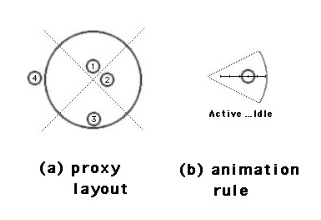
\includegraphics[width=0.5\linewidth]{figures/babble.png}
        \caption{The illustration on the left shows the layout of the proxy in Babble \cite{ericksonSocialTranslucenceApproach2000}, where dots 1, 2, and 3 are part of the conversation, and 4 is in another. The illustration on the right shows how the dots animate and drift further away depending on their activity level.}
        \label{fig:babble}
    \end{figure}

    \subsection{Workspace Awareness} \label{sec:sota_awareness}
    
    Endsley \cite{endsleyTheorySituationAwareness1995} defines \textit{awareness} as "\textit{knowing what is going on.}" Several traits have emerged in previous studies on awareness \cite{adamsSituationAwarenessCognitive1995, normanThingsThatMake1993, endsleyTheorySituationAwareness1995, gutwinDescriptiveFrameworkWorkspace2002}: Awareness is the knowledge about the state of the environment in both space and time. Since environments change over time, maintaining and updating this knowledge is part of awareness. Individuals can achieve this by interacting with and exploring the environment. Finally, awareness is not the primary goal of a task-oriented system but rather a secondary goal, the primary objective being to complete the task.

    Situation Awareness (SA) is a concept that arose in research about more dynamic and complex environments with high information load, variable workload, and risk \cite{gabaSituationAwarenessAnesthesiology1995}. Adams et al. \cite{adamsSituationAwarenessCognitive1995} define SA as "\textit{the up-to-the-minute cognizance required to operate or maintain a system.}" Endsley \cite{endsleyTheorySituationAwareness1995} describes a three-stage definition of SA that focuses more on the process. The first stage is the perception of relevant elements in the environment. The second stage is the comprehension of the current situation, or the ability to relate perceptual information retrieved in the first stage with past knowledge to understand their meaning. The third and last stage is the forecast of the status of those elements, which is invaluable for decision-making.
    
    Gutwin and Greenberg \cite{gutwinDescriptiveFrameworkWorkspace2002} define the concept of workspace awareness as "\textit{the up-to-the-moment understanding of another person's interaction with the shared workspace.}" It is a specialized kind of SA due to the shared workspace context -- it is about being aware not only of the environment but also of other individuals and their interactions with that environment. Similarly to Erickson and Kellog \cite{ericksonSocialTranslucenceApproach2000}, they believe the difficulty of maintaining awareness in collaborative tasks in digital systems lies in the technological constraints of the medium, the lack of information due to the limited perception of others, and the misrepresentation of that information.

    To aid the understanding of concepts and purposes of designing workspace awareness in groupware systems, Gutwin and Greenberg \cite{gutwinDescriptiveFrameworkWorkspace2002} developed a three-part conceptual framework. The first part focuses on what information is used and what is necessary for workspace awareness. The second part is about how that information is gathered. Lastly, the third part concerns the application of workspace awareness in collaboration.

    Previous research \cite{dourishAwarenessCoordinationShared1992, sohlenkampIntegratingCommunicationCooperation1994, mcdanielAwarenessCollaborativeSystems1997, gutwinDescriptiveFrameworkWorkspace2002} explore a set of workspace information that people keep track of during collaborative work, which is the elements that answer the questions "\textit{who, what, where, when, and how.}" Gutwin and Greenberg \cite{gutwinDescriptiveFrameworkWorkspace2002} present specific elements and questions answered by those elements according to what they believe is the core of workspace awareness, seen summarized on tables \ref{tab:workspaceElementsPresent} and \ref{tab:workspaceElementsPast}.

   \begin{table}[!ht]
        \centering
        \caption{Elements of workspace awareness of the present \cite{gutwinDescriptiveFrameworkWorkspace2002}.}
        \begin{tabular}{lll}
             \hline
             Category & Element & Questions \\
             \hline
             Who & Presence  & Is anyone in the workspace? \\
             & Identity  & Who is participating? Who is that? \\
             \vspace{0.7em}
            
             & Authorship & Who is doing that? \\
             What & Action & What are they doing? \\
             & Intention & What goal is that action part of? \\
             \vspace{0.7em}
            
             & Artifact & What object are they working on? \\
             Where & Location & Where are they working? \\
             & Gaze & Where are they looking? \\
             & View & Where can they see? \\
             & Reach & Where can they reach? \\
        \end{tabular}
        \vspace{1em}
        
        \label{tab:workspaceElementsPresent}

        \bigskip
        \caption{Elements of workspace awareness of the past \cite{gutwinDescriptiveFrameworkWorkspace2002}.}
        \begin{tabular}{lll}
             \hline
             Category & Element & Questions \\
             \hline
             How & Action history & How did that operation happen? \\
             \vspace{0.7em}
              & Artifact history & How did this artifact come to be in this state? \\
            \vspace{0.7em}
             When & Event history & When did that event happen? \\
             \vspace{0.7em}
             Who & Presence history & Who was here, and when? \\
             \vspace{0.7em}
             Where & Location history & Where has a person been? \\
             \vspace{0.7em}
             What & Action history  & What has a person been doing? \\
            
        \end{tabular}
        \vspace{1em}
        \label{tab:workspaceElementsPast}
    \end{table}


    Earlier findings \cite{segalEffectsChecklistInterface1994, normanThingsThatMake1993, dixHumanComputerInteraction2003, hutchinsTechnologyTeamNavigation1990, gutwinDescriptiveFrameworkWorkspace2002} propose three primary sources and mechanisms for gathering workspace information: through people's bodies and consequential communication, through workspace artifacts and feedthrough, and through conversation, gestures, and intentional communication. People's bodies provide extensive details about their current work, making watching and hearing other people a mechanism for obtaining workspace information \cite{gutwinDescriptiveFrameworkWorkspace2002, segalEffectsChecklistInterface1994}. This mechanism for gathering information is called \textit{consequential communication} \cite{segalEffectsChecklistInterface1994}.

    The second source of information is the artifacts produced in the workspace \cite{dixHumanComputerInteraction2003, gaverSoundSupportCollaboration1991}. The information that can be collected from these artifacts can be obtained either through visible characteristics \cite{gutwinDescriptiveFrameworkWorkspace2002} or through the sound that is made when manipulating them \cite{gaverSoundSupportCollaboration1991}. The mechanism used for gathering this information is called \textit{feedthrough} \cite{dixHumanComputerInteraction2003}, meaning that when manipulating an artifact, information is received by not only the person doing the action as a form of feedback but also by others who are watching.

    The third source of workspace information is conversation and gesture through intentional communication \cite{clarkUsingLanguage1996, heathUnpackingCollaborationInteractional1994, birdwhistellIntroductionKinesicsAnnotation1952}. People can gather information from verbal communication in different ways: through explicit conversational exchange of awareness elements \cite{gutwinDescriptiveFrameworkWorkspace2002}, by picking up relevant information from other peoples' conversations \cite{gutwinDescriptiveFrameworkWorkspace2002}, or through \textit{verbal shadowing} or "\textit{outlouds}" \cite{heathUnpackingCollaborationInteractional1994} which are comments made by individuals while working that are addressed to no one in particular.

    Gutwin and Greenberg \cite{gutwinDescriptiveFrameworkWorkspace2002} suggest five types of activities that benefit from workspace awareness. The identified types include: the management of coupling -- the degree to which people are working together \cite{salvadorDenverModelGroupware1996} or the amount of work a person can do before requiring the help of another \cite{gutwinDescriptiveFrameworkWorkspace2002}; simplification of communication -- allowing using deictic references, demonstrations, and visual evidence; coordination of actions; anticipation; and assistance.

    % compare workspace awareness and awareness

    \subsection{Spatial Group Interaction in VR} \label{sec:sota_spatial}

    Unlike conventional CSCW settings, real-time collaboration in virtual environments introduces novel interaction possibilities, particularly when multiple users simultaneously engage with one or more objects \cite{brollInteractingDistributedCollaborative1995}. Therefore, it becomes essential to acknowledge the importance of enhancing awareness in this specific context.

    A spatial approach to collaborative virtual environments consists of spaces or rooms allowing individuals to navigate and engage with one another and the objects, or artifacts, within these designated areas \cite{benfordSpatialModelInteraction1993}. With the goal of enhancing collaboration and scalability within large virtual environments, Benford and Falhén \cite{benfordSpatialModelInteraction1993} propose the spatial model of interaction. 

    The spatial interaction model introduces the concepts of medium, aura, awareness, focus, nimbus, and adapters. The medium is the means through which interactions with objects occur, for example, through text, audio, or visuals. The aura represents an area in which objects can interact within a given medium. When two auras collide, the interaction between the objects in the medium becomes possible. Objects can have multiple auras, such as their size, shape, and color.

    Awareness is the basis on which objects control their potential interactions, as determined by their auras. This awareness is not necessarily symmetrical. For example, between object A and object B, object A can be more aware of B than B is aware of A. The awareness of an object towards another is calculated based on the combination of its focus and nimbus. Focus and nimbus are, like auras, subspaces of an object and describe its attention or presence, respectively. Benford and Falhén \cite{benfordSpatialModelInteraction1993} describe this as "the more an object is within your focus, the more aware you are of it and the more an object is within your nimbus, the more aware it is of you".

    Furthermore, Benford and Falhén \cite{benfordSpatialModelInteraction1993} denote that a person does not need to be aware of their aura, focus, and nimbus, as these may be manipulated using natural interactions. Notably, they indicate three main ways of managing these subspaces. The first is through implicit interaction derived from, for example, the movement, orientation, or eye gaze of individuals. The second is through explicit adjustment of parameters, for instance, with the help of a user interface. The third is through adapters which modify a user's aura, focus, and nimbus. An example of an adapter would be a tool that a person can pick up or a table in which a user can sit, altering the user's aura, focus, and nimbus for that context.

    Domingues et al. \cite{dominguesCollaborative3DInteraction2011} develop a workflow-based approach to collaborative 3D interaction based on the spatial model of interactions. They describe the workflow concept, which manages tasks and ensures coordination in collaborative environments. The workflow comprises two components: the shared component, encompassing the data and state information of all users and sources within the environment; and the motor component, which uses the data from the shared component to execute actions on particular sources through assistance functions. Here, a \textit{source} is an object that users can perceive, \textit{particular sources} are objects that change during 3D interaction through assistance functions, serving as support tools, and \textit{assistance functions} help manage coordination in 3D interaction.

    \begin{figure}[h]
        \centering
        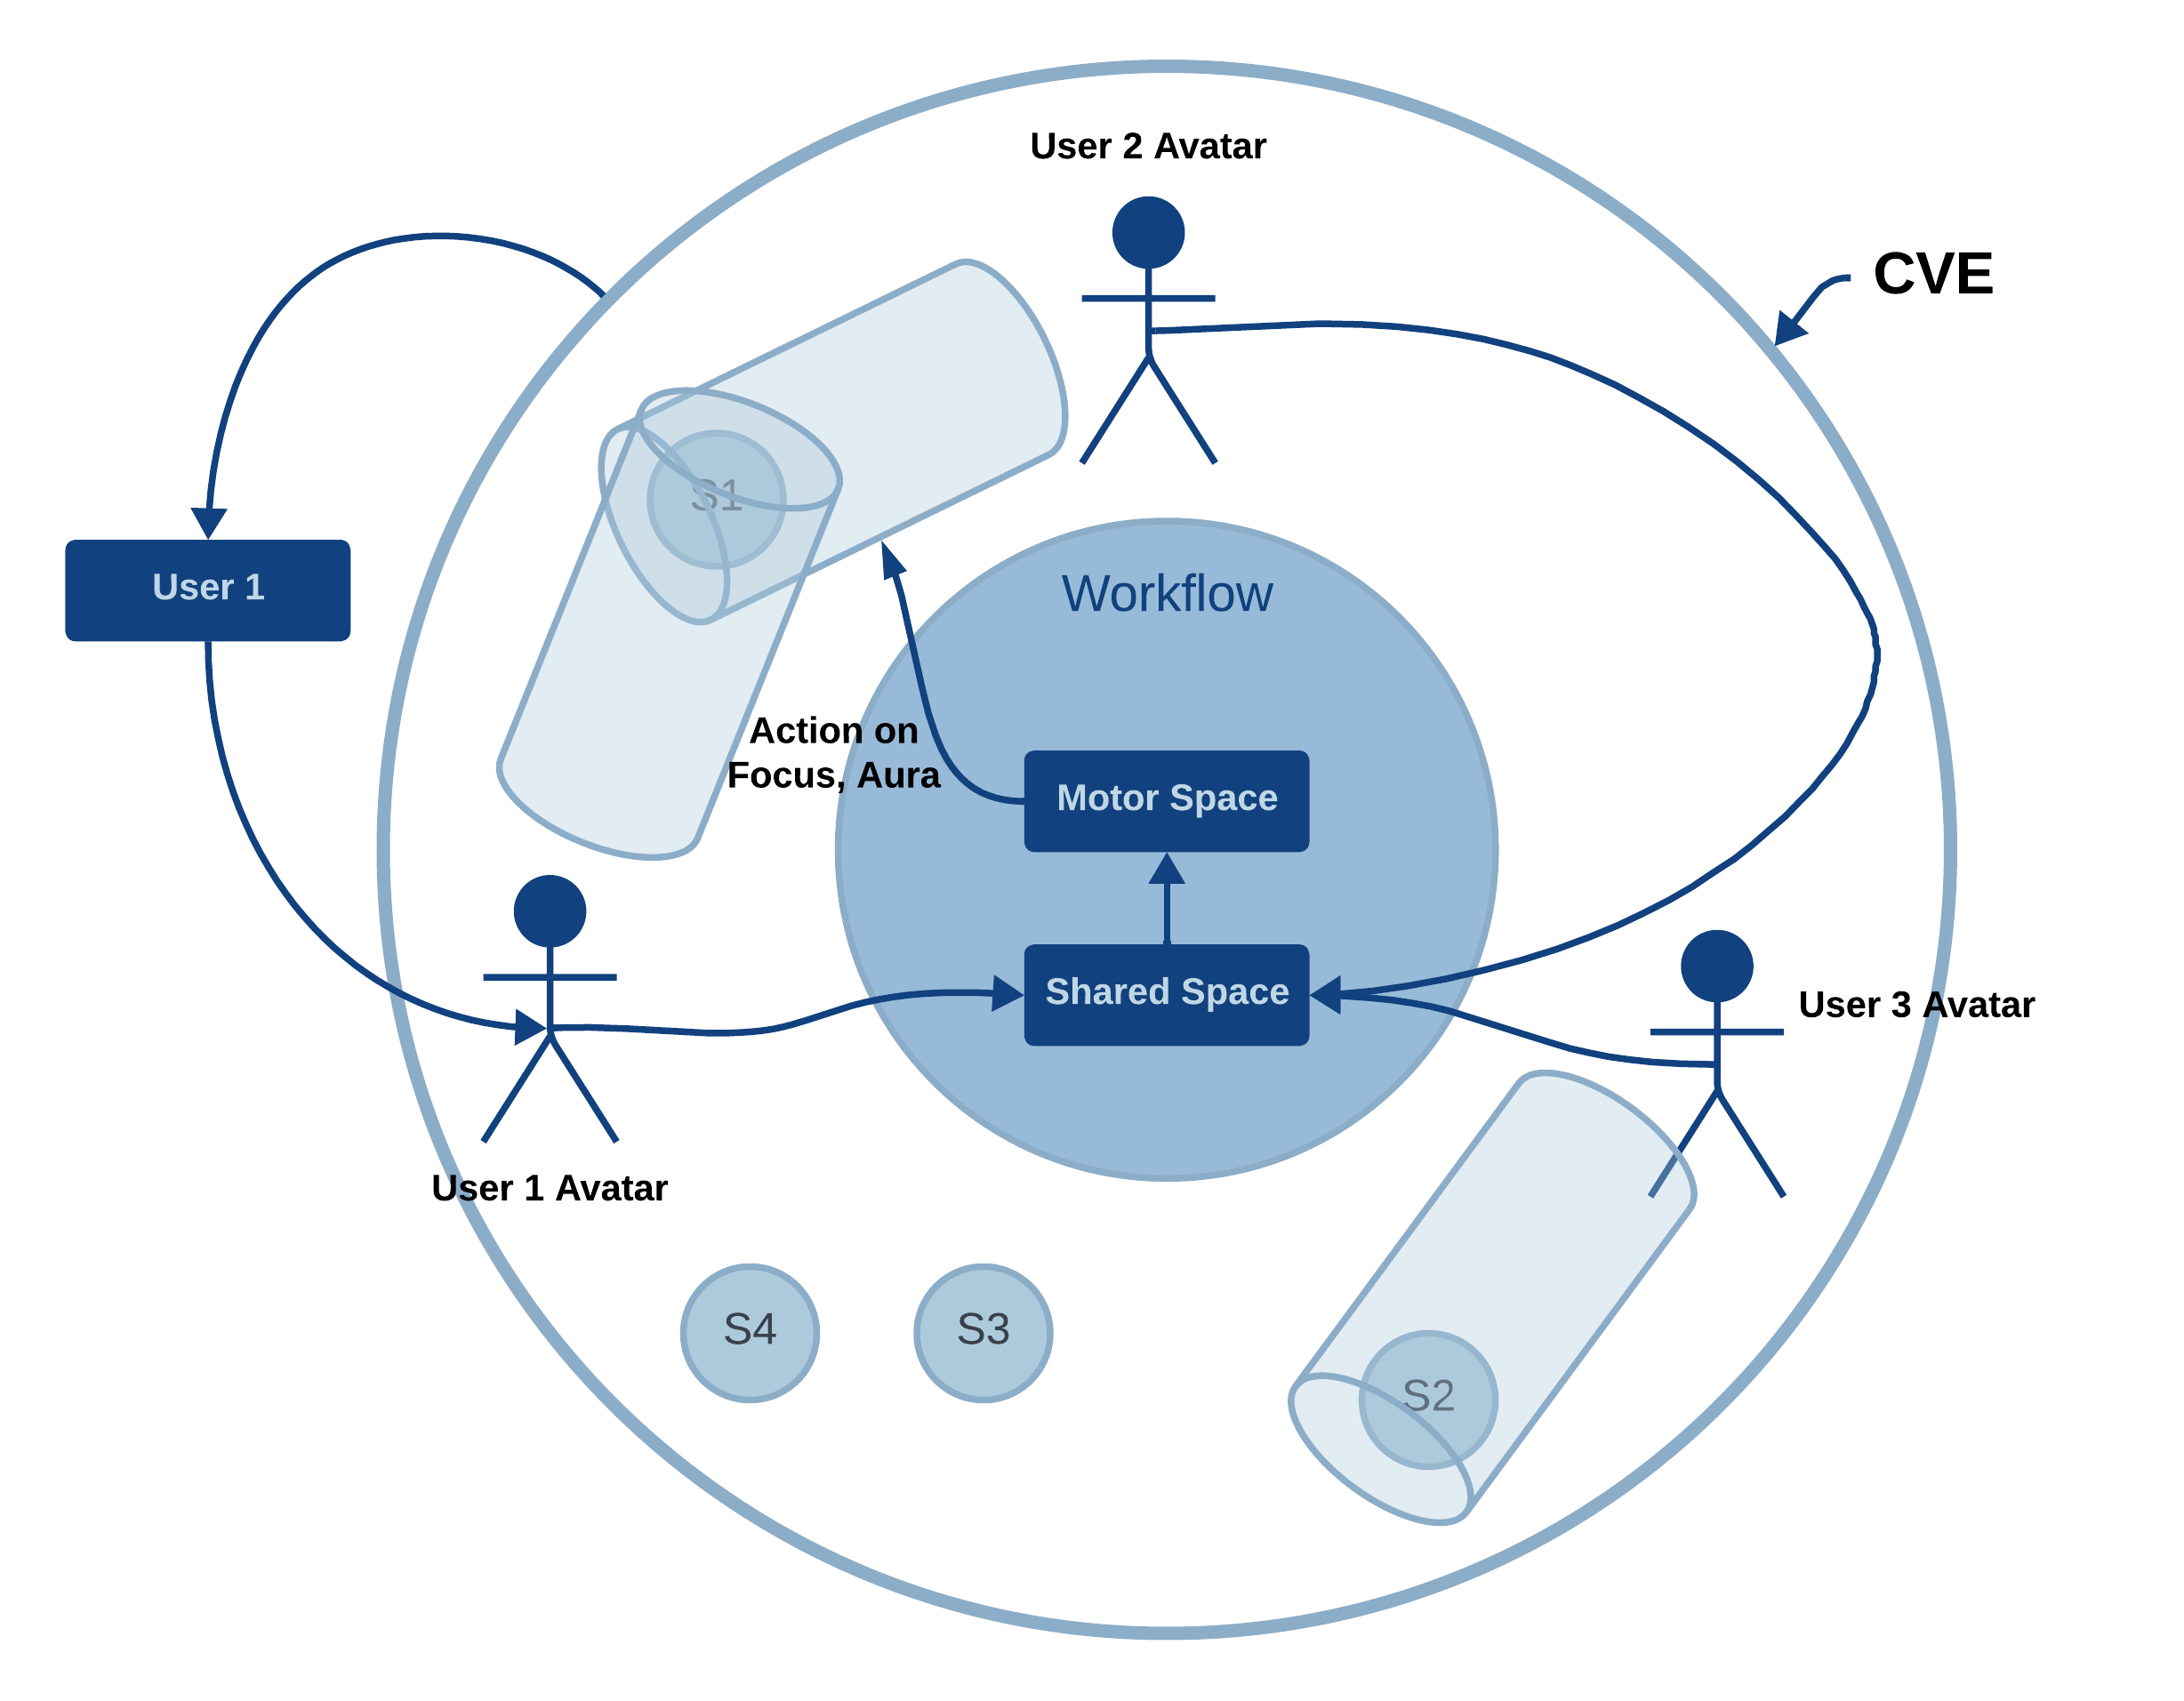
\includegraphics[width=0.9\textwidth]{figures/spatial_model.png}
        \caption{Portrayal adapted from the work of Domingues et al. \cite{dominguesCollaborative3DInteraction2011}. This represents their workflow approach applied to a CVE, where cylinders represent user foci. In this example, the nimbus of the object S1 is the set of users 1 and 2. }
        \label{fig:spatial_model}
    \end{figure}

    Next, they specify five particular sources, dedicated to interaction in the virtual environment. \textit{3DIFocus} coincides with objects the user can interact with, meaning in their field of view. \textit{3DINimbus} symbolizes all users that might interact with this source. \textit{3DIAura} is a zone that enables specific interactions if users are situated within its area. \textit{3DIAssistant} assists users during specific actions through a virtual guide. Lastly, \textit{3DIAvatar} is the digital counterpart of a user. These concepts are illustrated in figure \ref{fig:spatial_model}

    Using this model, Domingues et al. \cite{dominguesCollaborative3DInteraction2011} describe several assistance functions, in particular, an assistance function for helping the coordination of multi-user interaction with an object. They model multi-user interaction by inserting joints between the user avatars and the object, allowing for manipulation of that object using single-user interaction techniques. The assistance function then helps manage this interaction by creating visual guides for the users by changing the color of the avatars engaged in multi-user interaction, or by displaying the object's direction, for instance.
    
%\section{Object Interaction Techniques} \label{sec:sota_interaction}
\begin{comment}
    Bowman and Hodges \cite{bowmanFormalizingDesignEvaluation1999} present a taxonomy of object interaction techniques, categorizing them into three main groups: selection -- choosing an object; release -- releasing an object; and manipulation -- setting the position, orientation, or other characteristics of the selected object. Object manipulations are accomplished by mapping user input, either through physics simulation or programmed behavior  \cite{mendesSurvey3DVirtual2019}. This section primarily details techniques within the manipulation group that involve programmed behaviors, with a few also encompassing selection features.

    Mendes et al. \cite{mendesSurvey3DVirtual2019} extend the taxonomy to differentiate various mapping mechanisms employed in object manipulation techniques. In terms of transformation separation, these mechanisms can be categorized as follows: no transformation separation -- when interactions do not separate degrees of freedom (DoF), \textit{partial} -- when some interactions group DoFs while separating others, and \textit{total} -- when all transformations are applied separately. A study by Mendes et al. \cite{mendesBenefitsDOFSeparation2016a} analyzed the advantages of DoF separation in mid-air 3D object manipulation. The findings indicated that this separation reduced errors while increasing the time required for complex tasks, rendering it more suitable for tasks demanding precision. This conclusion can be extended to other manipulation mediums, such as tabletop interactions.

    Regarding transformation mapping, Mendes et al. \cite{mendesSurvey3DVirtual2019} distinguish between the following approaches: \textit{exact} -- mapping user input directly to the virtual object, \textit{scaled} -- a linear or nonlinear mapping to either increase accuracy with closer objects or increase the range of movement with farther objects, \textit{remapping} -- mapping DoFs onto different DoFs, and \textit{hybrid} -- using a combination of other mapping types for different DoFs.

    Numerous previous studies have investigated the effectiveness of touch-based interactions in the context of DeskVR, exploring various scenarios such as menu navigation \cite{zielaskoMenusDeskSystem2019}, medical image data examination for radiologists \cite{sousaVRRRRoomVirtualReality2017}, travel techniques \cite{amaroDesignEvaluationTravel2022}, and object interaction \cite{almeidaSIT6IndirectTouchbased2023}. The consensus from these studies suggests that, although a touch-based approach may not always be the most time-efficient, it significantly reduces physical strain, enhancing overall comfort and prolonged usage time for individuals. This aspect is essential for DeskVR, where the primary objective is to alleviate physical strain, improve accessibility, and boost productivity \cite{zielaskoRemainSeatedFullyimmersive2017, zielaskoSitNotSit2021}. For this reason, touch-based approaches will be preferred over mid-air interactions.

    It is important to note that touch-based approaches are commonly classified as direct and indirect touch manipulation \cite{mendesSurvey3DVirtual2019}. Direct touch involves users manipulating an object by touching it through a screen display. However, this is impractical in HMD VR, where users cannot see the touch display. Therefore, the most suitable approach is indirect touch manipulation, where users utilize an external touch surface without the need to touch the object directly.
    
    This section is divided into two parts: first, an overview of techniques for single-user object interaction, and second, a discussion of techniques designed for manipulating objects in a multi-user context.

    \subsection{Single User}

    There is a recurring theme in collaborative VR research \cite{pinhoCooperativeObjectManipulation2002, pinhoCooperativeObjectManipulation2008, mortensenCollaborationTeleImmersiveEnvironments2002, otmaneCollaborative3DInteraction2007} that emphasizes a preference for employing single-user techniques in collaboration rather than designing specific multi-user approaches. The rationale behind this choice is to allow users to utilize techniques that are more familiar and easier for them to understand, as these approaches are extensively researched and widely known. As such, an examination of single-user interaction is relevant.

    % mid-air

    \cite{bowmanEvaluationTechniquesGrabbing1997, wilkesAdvantagesVelocitybasedScaling2008}
    \cite{mendesBenefitsDOFSeparation2016a}

    % touch
    
    \cite{martinetEffectDOFSeparation2010}
    \cite{sousaVRRRRoomVirtualReality2017}
    \cite{simeoneIndirectTouchManipulation2016}
    \cite{almeidaSIT6IndirectTouchbased2023}

    \subsection{Multi-User}

    \cite{riegeBentPickRay2006}
    \cite{duvalSkeweR3DInteraction2006}
    \cite{chenechalWhenGiantMeets2016}
    \cite{grandiDesignEvaluationHandheldbased2017}
\end{comment}

\section{Concurrency Control} \label{sec:sota_concurrency}

    Margery et al. \cite{margeryGeneralFrameworkCooperative1999} developed a classification to assess the cooperation levels in multi-user systems. In systems with level 1 collaboration, users can perceive and communicate with each other in the virtual world through avatars. Level 2 systems enable users to manipulate objects within the scene. Level 3 systems allow users to manipulate the same object simultaneously. Level 3 can be further subdivided based on the degree of independence in users' actions, such as independently changing different aspects of an object or combining inputs codependently. This last collaborative level, particularly the codependent mode, is considered the most natural and immersive form of collaboration, offering enhanced efficiency.
    
    Broll \cite{brollInteractingDistributedCollaborative1995} had previously defined something similar to levels 2 and 3, cooperative and collaborative interaction, respectively. Recognizing which interactions are concurrent and which are not is essential yet challenging. Without a notion of simultaneity, interactions become a series of individual moves by each user rather than a coordinated combination. In distributed environments, typical in collaborative virtual reality, where each user has a copy of the world, determining concurrency is complicated, especially considering communication delays.
 
    Concurrency control prevents conflicts of concurrent updates arising from adverse network conditions. In its absence, users manipulating shared objects in conflicting directions may experience difficulty anticipating outcomes and encounter divergence of state \cite{robertsControllingConsistencyCollaborative2004}, introducing confusion among participants, offering disparate views of what should be a shared world and, in turn, violating the essential consistency requirement \cite{sungConcurrencyControlCIAO1999}. Therefore, the study of concurrency control emerges as an essential research topic for developing systems with level 3 collaboration.

    The following subsections describe three distinct approaches for implementing concurrency control. Object ownership methods use locking mechanisms to block users from interacting with an object or its properties unless they possess a corresponding lock or ownership. Attribute separation methods assign specific attributes or degrees of freedom of an object to individual users, making each user responsible for that attribute. Finally, distributed average techniques calculate the average of participants' actions, integrating and updating them distributively.

    \subsection{Object Ownership Techniques}

    Greenberg and Marwood \cite{greenbergRealTimeGroupware1994} describe how traditional concurrency control strategies can be used in real-time groupware systems. In particular, they demonstrate how the method of privileged access through locking can be applied in these systems, describing two different approaches. A non-optimistic locking policy blocks users from interacting with an object until a lock has been granted, signifying ownership over the object. An optimistic locking policy allows users to manipulate an object before they know if a lock has been granted to them. If the lock has been denied, the object returns to its original state, and a repair must be done. Optimistic locking schemes can be further divided into two approaches. A fully-optimistic approach allows users to manipulate multiple objects with tentative locks, while a semi-optimistic approach only allows users to manipulate one object at a time.

    BrickNet \cite{singhBrickNetSoftwareToolkit1994a} is a toolkit for network-based virtual environments. It uses a pessimistic locking mechanism for object manipulation where objects can only be updated by the current owner. Users have to request ownership over an object to the server, and the server mediates object updates. DIVE \cite{hagsandInteractiveMultiuserVEs1996} is a multi-user distributed virtual environment system. DIVE also employs a pessimistic locking mechanism, similar to BrickNet, where users require an object-based token to interact with the object. Spline \cite{watersDiamondParkSpline1997} is a software platform for developing distributed virtual environments that implements the Interactive Sharing Transfer Protocol, or ISTP \cite{watersDesignInteractiveSharing1997}. Objects in the ISTP protocol, like DIVE, are only subject to changes from its owner process. This ownership can be transferred between processes. CAVERNsoft \cite{leighCAVERNDistributedArchitecture1997} is a collaborative software architecture that was used by the CAVE Research Network, which also uses the pessimistic locking approach.

    The PaRADE collaborative environment \cite{robertsMaximisingConcurrencyScalability1997, robertsControllingConsistencyCollaborative2004} takes a different approach to pessimistic locking by employing a predictive strategy. Developed to mitigate adverse network effects, PaRADE aims to enhance both responsiveness and consistency through advanced time management. In PaRADE, all events are timestamped with both wall-clock time and causal time, and efforts are made to predict events to reduce the impact of network delays. Combining these times is used for sufficient causal ordering, serving as a middle ground for Lamport's causal ordering \cite{lamportTimeClocksOrdering1978} to enhance concurrency and responsiveness. This approach restricts changes to an object to originate from a single user, leading to the adoption of a predictive object transfer paradigm that anticipates entity ownership in advance.

    The predictive object ownership transfer relies on application knowledge and heuristics to anticipate a user's intention to interact with an object, enabling the transfer in advance of the ownership to minimize the impact of network delays. This advance transfer is important for optimizing responsiveness and in scenarios where ownership may have been erroneously transferred, allowing for retransmission to the correct recipient. Yang and Lee \cite{yangScalablePredictionBased2000} identified scalability challenges in the widespread dissemination of token requests to all users in the network. In response, they introduced the concept of an entity radius, wherein messages are selectively delivered only to individuals within this radius, forming an "entity-centric multicast group."
    
    Pessimistic approaches for locking mechanisms help preserve data integrity in databases, for example. However, in settings such as collaborative virtual environments (CVEs), not only does obtaining a lock necessitate user waiting, but ensuring sequential updates becomes less scalable with a growing number of users. Sung et al. introduce CIAO \cite{sungConcurrencyControlCIAO1999}, a large-scale 3D layout system that uses a semi-optimistic policy for managing shared object manipulation to enhance responsiveness. Unlike traditional systems, users in CIAO can manipulate objects without waiting for a lock. To address potential confusion arising from multiple users interacting with an object, the CIAO interface incorporates awareness features, using translucent clones to indicate ongoing manipulations yet to be validated. The authors also address the challenges of concurrently interacting with hierarchically related objects.
    
    \subsection{Attribute Separation Techniques} \label{sec:dof_concurrency}

    The approaches discussed in the previous section are limited to a collaboration level of 2, as there is no stage where multiple users synchronize their inputs on a shared object. Additionally, those concurrency control mechanisms often introduce issues commonly called "surprise" \cite{linebargerConcurrencyControlMechanisms2004}. Such surprises manifest as conflicts leading to the reversal of changes or unexpected alterations in the anticipated order of events due to concurrency control conflicts. 
    
    This section introduces strategies that elevate collaboration to level 3, enabling independent modifications of various attributes of an object simultaneously. The concept involves assigning ownership of specific attributes to individual users, allowing multiple users to collaboratively manipulate an object without needing sequential ownership.
    
    In their work, Lee et al. \cite{leeSupportingFineGrainedConcurrent2012} refer to the manipulation of an attribute of a shared object as a "task." However, they explain the importance of avoiding "surprises" or, in this context, "task-surprises." These surprises may arise when interruptions occur during user tasks by other tasks or when task dependencies result in unexpected states when executed concurrently.

    \begin{figure}[h!]
        \centering
        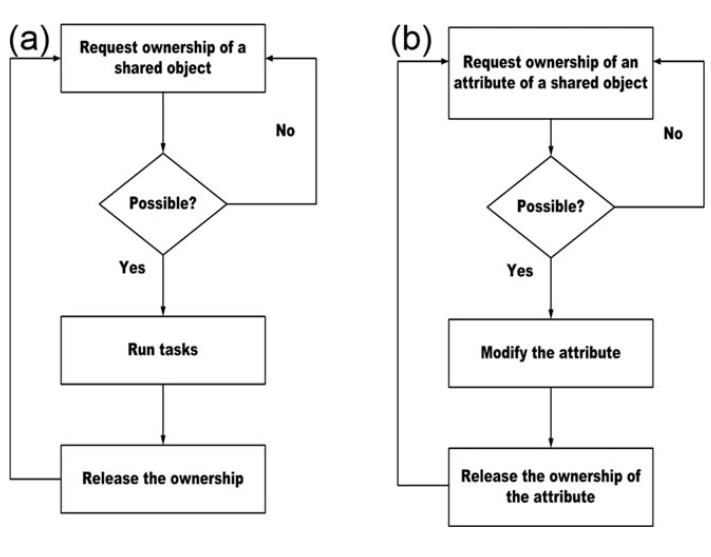
\includegraphics[width=0.65\linewidth]{owner_vs_attr_2.png}
        \caption{Illustration depicting the difference between ownership transfer and attribute separation \cite{leeSupportingFineGrainedConcurrent2012}.}
        \label{fig:enter-label}
    \end{figure}

    % TODO: I am mixing here distributed and dof techniques, can't really think of a nice way of doing this introductory part
    Advancements in internet infrastructure around the turn of the century, particularly with the establishment of Internet2 \cite{yeungInternetScalingBackbone1997} -- a robust network implemented in the United States in 1996 for academic purposes -- sparked new interest in exploring collaborative tasks in remote environments. Mortensen et al. \cite{mortensenCollaborationTeleImmersiveEnvironments2002} aimed to assess the feasibility of joint tasks when two users, separated by thousands of miles, interacted in a shared virtual environment within DIVE. The specific task involved both users lifting a stretcher together and moving it along a predefined path into a building. To achieve this, two handles were added to the stretcher for the users to manipulate, with the stretcher aligning itself based on the position and orientation of these handles. Their findings revealed that while data transmission speeds and throughput were sufficient, the lack of software support, particularly concerning lost data packets impacting consistency, posed a significant challenge.

    Roberts et al. \cite{robertsConstructingGazeboSupporting2003} investigated two distinct methods of shared object manipulation and how these methods were influenced by the display devices their users employed: an immersive walk-in display with tracked head and hands, and a desktop application. The two methods explored were sharing the same attribute and sharing through different attributes. To conduct this study, they devised an experiment where users collaborated on constructing a gazebo in DIVE. Some sub-tasks required users to collaborate using the same attribute, such as jointly carrying a beam, while other tasks involved simultaneous manipulation of the object for different purposes, such as one person inserting a screw while another held the beam in place. This study also concluded that technological advancements had made such collaborative tasks feasible, but the ownership mechanism of DIVE failed to provide effective collaboration \cite{robertsSupportingCloselyCoupled2005a}. As such, it became evident that new systems needed to be developed with level 3 collaboration in mind.

    Pinho et al. \cite{pinhoCooperativeObjectManipulation2002, pinhoCooperativeObjectManipulation2008} proposed a method for collaborative object interaction by separating degrees of freedom (DoF) and assigning them to different users. A degree of freedom in this context refers to a degree of control over the movement of an object, such as horizontal translation or rotation around an axis. As previously mentioned in section \ref{sec:sota_interaction}, the separation of DoF can be beneficial when precision is an important factor.
    
    The goal of this approach was to use single-user interaction techniques, such as HOMER \cite{bowmanEvaluationTechniquesGrabbing1997, mossel3DTouchHOMERSIntuitive2013}, in collaborative manipulation, with the reasoning that they were well-researched, commonly understood, and perceived as more "magical" than natural, which was prevalent in most collaborative manipulation techniques then. The objective was to extend users' capabilities for multi-user object interaction. Additionally, the authors focused on awareness by implementing features like using a pointer to indicate the selected object, changing the object's color based on its state, and representing the DoF graphically, as shown in Figure \ref{fig:pointer}. While the results were positive, two challenges were identified: testing the applicability with more than two users, and the selection of DoF for each user was predetermined in a configuration, limiting flexibility.

    \begin{figure}[h!]
        \centering
        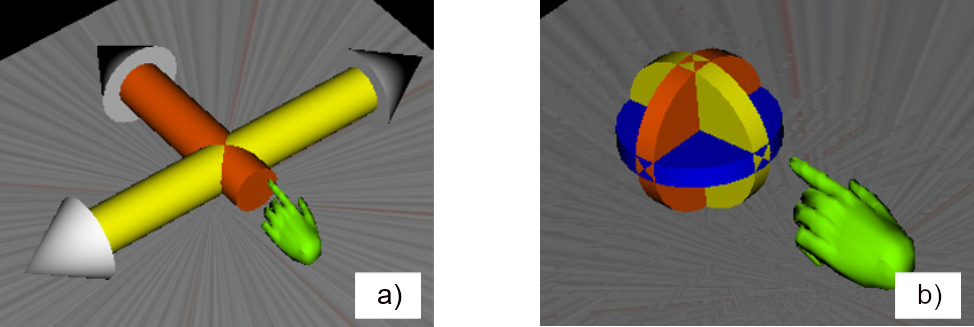
\includegraphics[width=.96\textwidth]{figures/pointer.png}
        \captionof{figure}{Illustration of translation (a) and rotation (b) pointers in \cite{pinhoCooperativeObjectManipulation2008}}
        \label{fig:pointer}
    \end{figure}
    

    Lee et al. \cite{leeSupportingFineGrainedConcurrent2012} proposed a concurrency control mechanism based on fine-grained tasks. In this approach, if a user who does not own an object requests a task to manipulate a shared object, the task is permitted if it avoids conflicts with the owner's task and does not lead to task surprises. If the task is not allowed, non-owners can perform their tasks with duplicates of the object on a personal workspace, similar to the ghost images in CIAO \cite{sungConcurrencyControlCIAO1999}. The outcomes of these modifications in personal workspaces can be stored, allowing users to discuss and determine the final state of the object. Figure \ref{fig:sota_finegrained} demonstrates the flow of the concurrency control process. 

    \begin{figure}[ht!]
        \centering
        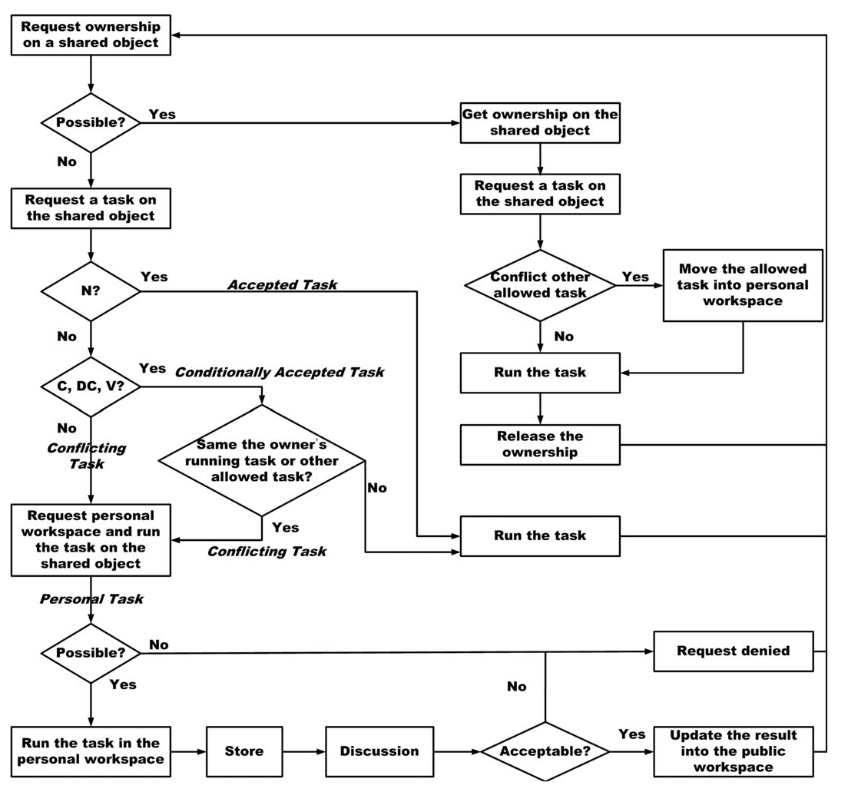
\includegraphics[width=1\linewidth]{figures/finegrainedtasks.png}
        \caption{Illustration of the fine-grained task concurrency control system by Lee et al. \cite{leeSupportingFineGrainedConcurrent2012}.}
        \label{fig:sota_finegrained}
    \end{figure}

     The allowance types for each task classification can be seen on Table \ref{tab:sota_finegrained}. \textit{Conflicting tasks} are exclusive to the object's owner. \textit{Conditionally accepted tasks} can be executed only if no one else is performing the task, while \textit{accepted tasks} can always be executed. While their implementation demonstrated slower efficiency compared to other attribute-sharing mechanisms, Lee et al.'s approach reduced the occurrence of task surprises.

    \begin{table}[h!]
        \centering
       \caption{Allowance type for each task classification by Lee et al. \cite{leeSupportingFineGrainedConcurrent2012}.}
        \begin{tabular}{m{12em} l}
            \hline
            Classification of Tasks & Allowance Type  \\
            \hline
            Translation & Conflicting task \\
            Rotation & Conflicting task \\
            Scaling & Conflicting task \\
            Fission & Conflicting task \\
            Merge & Conflicting task \\
            New & Accepted task \\
            Remove & Conflicting task \\
            Copy & Conditionally accepted task \\
            Data calculation & Conditionally accepted task \\
            Visual property & Conditionally accepted task \\
        \end{tabular}
 
        \label{tab:sota_finegrained}
    \end{table}
    
    \subsection{Distributed Average Techniques} \label{sec:average_concurrency}

    This section explores techniques associated with codependent level 3 collaboration. Integrating level 3 collaboration into CVEs is challenging, especially in regards to the complexity of combining and integrating actions from multiple users, the absence of feedback inherent in physical interactions with an object, and network communication issues, especially concerning latency, which significantly influences the ability to detect simultaneous actions \cite{ruddleSymmetricAsymmetricAction2002, brollInteractingDistributedCollaborative1995}.
    
    Ruddle et al. \cite{ruddleSymmetricAsymmetricAction2002} investigated whether an asymmetric or symmetric approach was better suited for level 3 collaboration in the piano mover's task. This task involves two users maneuvering a large virtual object through confined spaces. Symmetric manipulation requires coordinated actions in direction and intensity, while asymmetric manipulation allows users to interact with the object differently, considering the average of the interactions. To address latency concerns, experiments were conducted on a single host computer. Interestingly, the results did not reveal a significant difference in the time participants took to complete the task, but instead, that performance depended on the task. However, the study highlighted the challenge of coordinating participants' movements, emphasizing the need for feedback, whether haptic or otherwise.

    Friston et al. \cite{fristonConsensusBasedNetworking2022} present a concurrency control framework designed to enable the integration of level 3 collaboration in distributed virtual environments. This approach views the collaborative environment as a distributed data-fusion problem and incorporates elements such as prediction, distributed averaging, continuous authority, and constraint duplication. The methodology is rooted in consensus-based networking, where simulations share state updates with other nodes, and local solvers integrate these updates to establish a distributed average consensus of the system's state, ensuring consistency over time. Unlike bilateral operation or force-reflection systems, where clients submit inputs to a central authority, this approach calculates actions distributively, resulting in improved scalability. The authors conducted experiments that demonstrated the effectiveness of this technique in preserving causality, stacking objects, enabling level 3 collaboration, and providing support for haptic feedback.

\section{DeskVR Interaction} \label{sec:sota_interaction}

    Before the widespread adoption of stereoscopic displays, various effective approaches emerged for utilizing a multi-touch tabletop surface to interact with 3D objects with minimal fatigue \cite{benkoBalloonSelectionMultiFinger2007, strothoffTriangleCursorInteractions2011, daiberBalloonSelectionRevisited2012}. Balloon Selection \cite{benkoBalloonSelectionMultiFinger2007} employs the metaphor of manipulating a balloon attached to a string. This approach divides a 3DOF positioning task into a 2DOF positioning task with one finger on the touch surface and a 1DOF string-pulling task with the other finger to control the height of the balloon. Pulling the fingers apart decreases the balloon's height and bringing them together increases its height. Balloon selection does not differentiate between right and left hands; instead, it prioritizes the order in which fingers are placed on the surface, designating the primary finger (anchor), secondary finger (stretching finger), and tertiary finger (selection finger). This design allows both right-handed and left-handed users to use the technique effortlessly. Additionally, the stretching finger may not always be held, allowing the balloon's height to remain fixed when removed. This feature, referred to as "\textit{String Height Clutching}" by the authors, enables the extension of the balloon's height infinitely. This technique has shown low error rates, likely due to the user's hands being supported by the tabletop surface, resulting in significantly reduced hand tremor and arm fatigue.

    \begin{figure}[ht!]
        \centering
        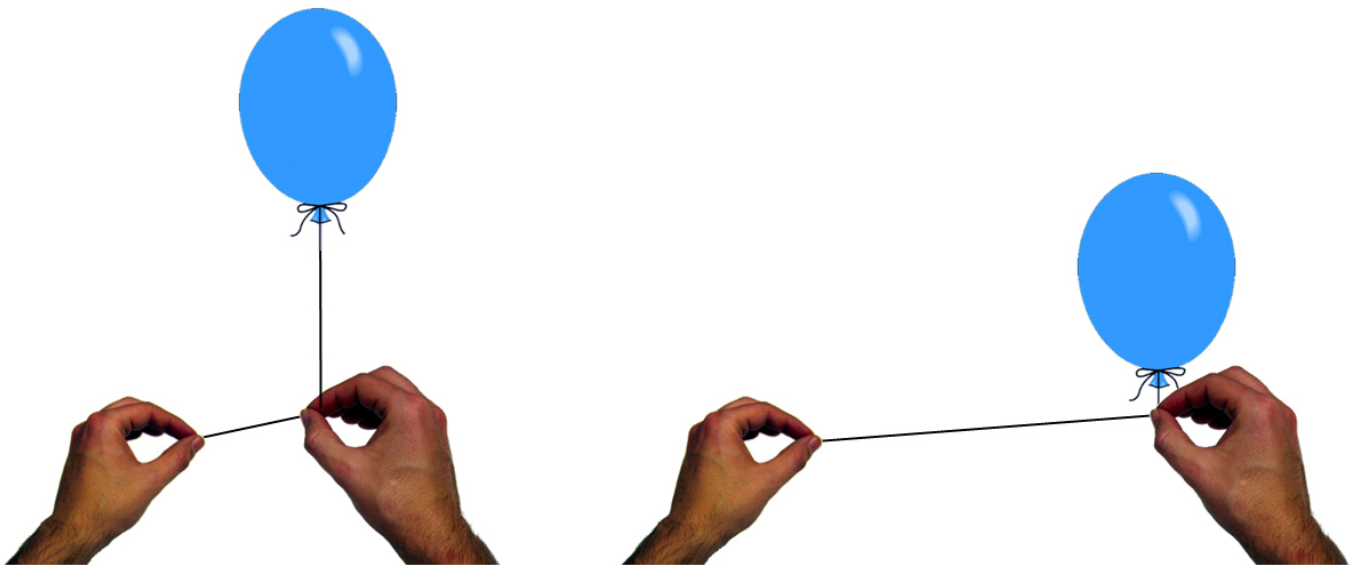
\includegraphics[width=1\linewidth]{figures/balloon_selection.png}
        \caption{Illustration of the Balloon Selection metaphor \cite{benkoBalloonSelectionMultiFinger2007}.}
        \label{fig:sota_balloon}
    \end{figure}

    Corkscrew Selection \cite{daiberBalloonSelectionRevisited2012}, similar to Balloon Selection, also breaks down the 3DOF task into a 2DOF positioning task and a 1DOF height task. However, it differs in the method used to adjust the height of the selection point, achieved through a rotational motion around a selection widget.
    
    Triangle Cursor \cite{strothoffTriangleCursorInteractions2011}, on the other hand, creates an isosceles triangle with its two base vertices positioned at the touch points of two fingers, while the altitude's base point is located at the midpoint. Manipulating the triangle's position involves moving the fingers on the surface, while adjusting its height is controlled by scaling the triangle similarly to a typical pinch gesture based on the distance between the two fingers. The height's upper limit is constrained by the diagonal of the touch surface. Additionally, users can initiate yaw rotation around an axis perpendicular to the table's surface by rotating the fingers around the midpoint.

    In their evaluation comparing Triangle Cursor to Balloon Selection, the authors noted a slight preference in terms of speed and error minimization for Triangle Cursor. However, it's worth mentioning that the tasks necessitated the use of rotational techniques, which required an extension of Balloon Selection by using the rotation of the secondary finger around the primary finger as rotational input.

    \begin{figure}[ht!]
        \centering
        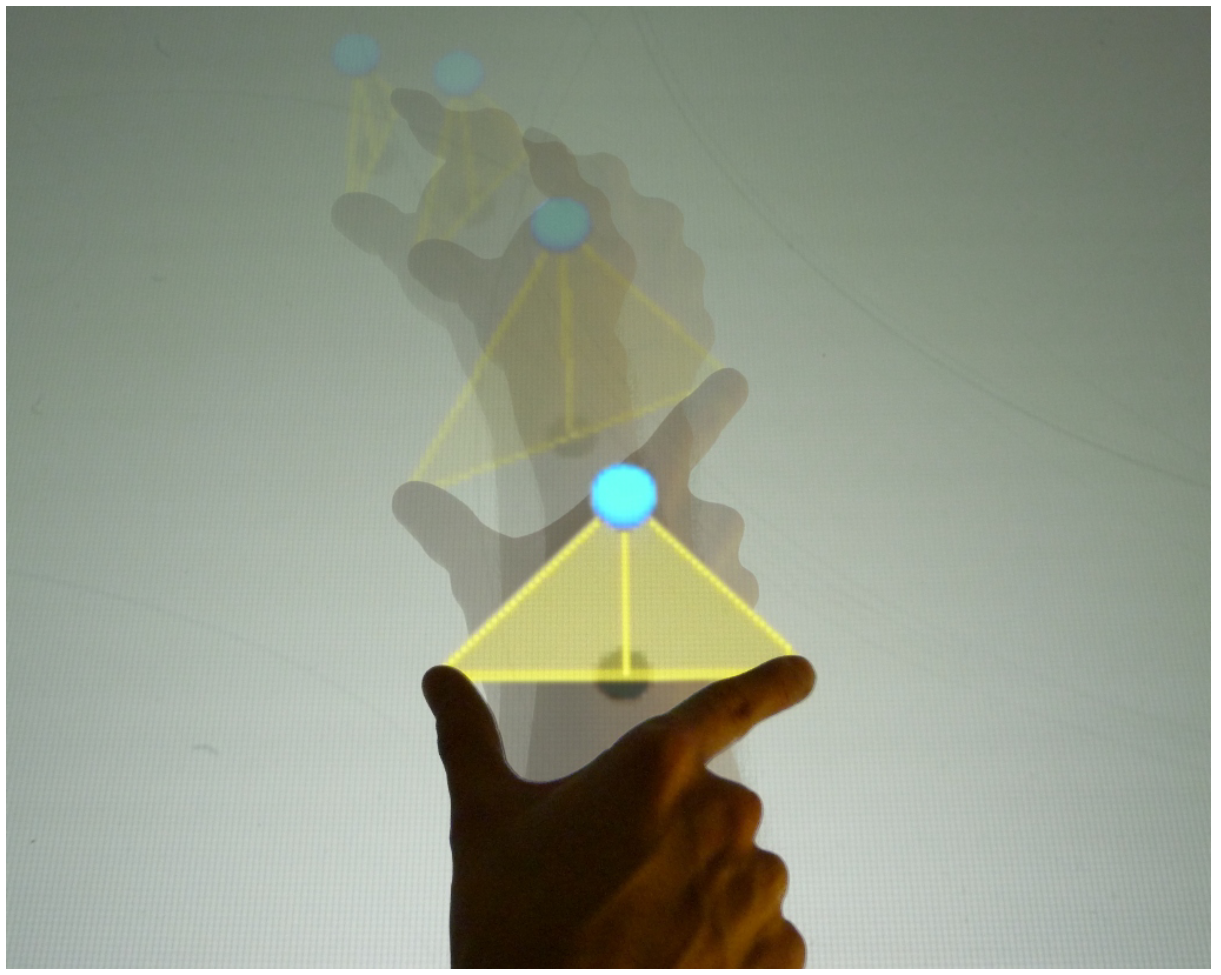
\includegraphics[width=0.6\linewidth]{figures/triangle_cursor.png}
        \caption{Illustration of the Triangle Cursor technique \cite{strothoffTriangleCursorInteractions2011}.}
        \label{fig:sota_triangle}
    \end{figure}


   Zielasko et al. \cite{zielaskoRemainSeatedFullyimmersive2017} introduced the concept of DeskVR, a fully immersive VR experience accessed entirely from an office desk while the user remains seated. Initially conceived to integrate with the workflow of data analysts, the application of this concept extends to broader applications, aiming to alleviate physical strain associated with standing, extend work periods, enhance accessibility, and boost overall productivity.

    Zielasko et al. \cite{zielaskoSitNotSit2021} surveyed to evaluate the advantages and disadvantages of standing versus sitting and the degree of embodiment in virtual reality experiences. The findings indicated that sitting generally scored higher in reducing cybersickness, enhancing comfort, ensuring safety, and improving accessibility. On the other hand, standing was preferred for perceived self-motion, locomotion preciseness, and engagement.

    Given the constraints of DeskVR, environmental interactions must be re-evaluated, especially regarding selection, manipulation, and travel techniques. Because users remain seated in DeskVR, this enables interactions not common in typical VR scenarios, such as touch-based interactions on a desk. Zielasko et al. \cite{zielaskoMenusDeskSystem2019} explored this concept through the evaluation of four menu interaction arrangements in DeskVR: "Desk" aligns menus with the virtual desk, "Air" aligns menus with the user's task, and "DeskPlus" and "AirPlus" combine the previous scenarios with a physical desk to provide passive haptics. These configurations can be seen in Figures \ref{fig:sota_desk_z} and \ref{fig:sota_desk_z2}. The results revealed diverse individual preferences for menu configurations. Some favored desk-aligned menus for tangibility, while others found it odd to touch a menu expected to be virtual. Additionally, menus aligned with the virtual desk required more head movement, making them less efficient. However, variants with a physical desk were favored for reducing physical strain.
    
    \begin{figure}[h!]
        \centering
        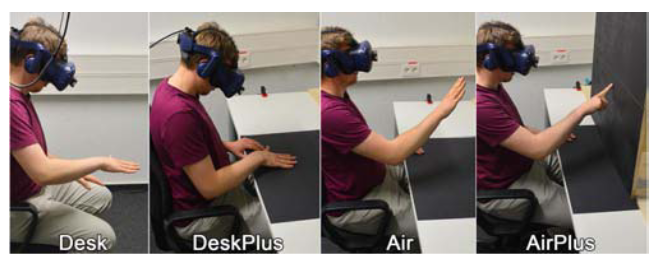
\includegraphics[width=0.85\linewidth]{figures/menu_desk.png}
        \caption{The four different scenarios studied in \cite{zielaskoMenusDeskSystem2019}. The "Desk" scenario aligns the menu with a virtual desk, while the "Air" scenario aligns the menu with the task. The "DeskPlus" scenario aligns the virtual desk with a physical desk, while "AirPlus" aligns the menu with the taks and a vertical board.  }
        \label{fig:sota_desk_z}
    \end{figure}

    \begin{figure}[h!]
        \centering
        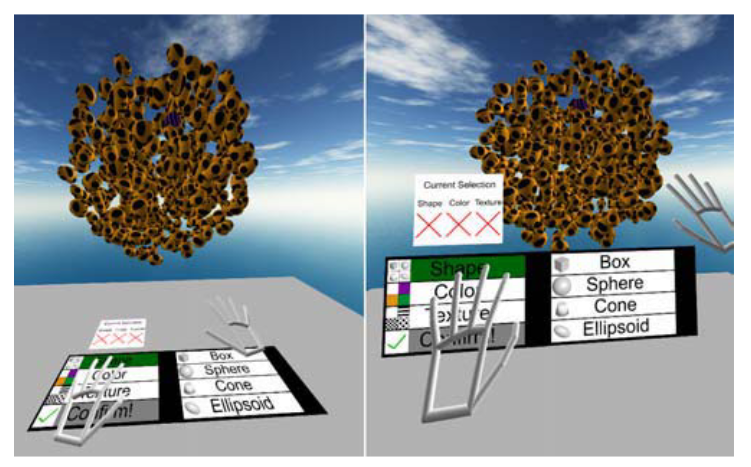
\includegraphics[width=0.85\linewidth]{sota_desk_menu.png}
        \caption{Experimental settings in \cite{zielaskoMenusDeskSystem2019} for desk-aligned menus on the left and task-aligned menus on the right.}
        \label{fig:sota_desk_z2}
    \end{figure}

    Sousa et al. \cite{sousaVRRRRoomVirtualReality2017} introduced VRRRRoom, a VR radiology reading room with a desktop surface for interacting with medical images. Medical images are displayed in 3D above a virtual desk and can be manipulated using indirect touch controls. Users can change volume slices and adjust brightness with their left hand, while rotating the image and changing the scale can be done with their right hand, as depicted in Figure \ref{fig:vroom_gesture}. The gesture-based interaction minimizes the need for users to move their head to view controls, as illustrated in Figure \ref{fig:vroom_desk}.

    \begin{figure}[h!]
        \centering
        \begin{minipage}[t]{.45\textwidth}
          \centering
          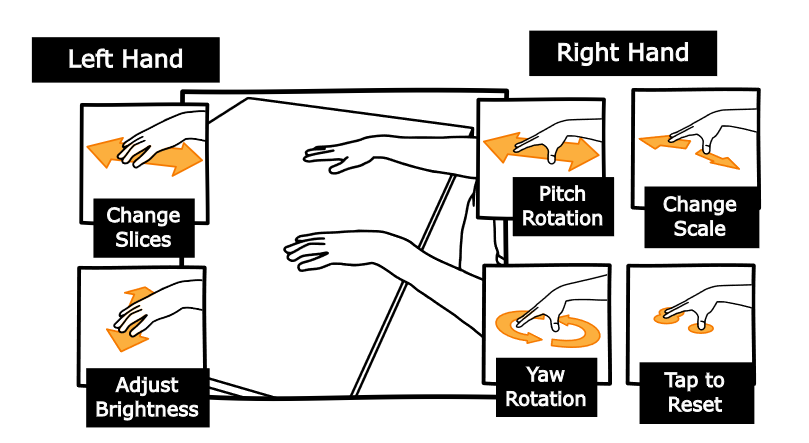
\includegraphics[width=1\textwidth]{figures/vroom_gesture.png}
          \captionof{figure}{Gesture dictionary in \cite{sousaVRRRRoomVirtualReality2017}}
          \label{fig:vroom_gesture}
        \end{minipage}%
        \hspace{0.05\textwidth}
        \begin{minipage}[t]{.45\textwidth}
          \centering
          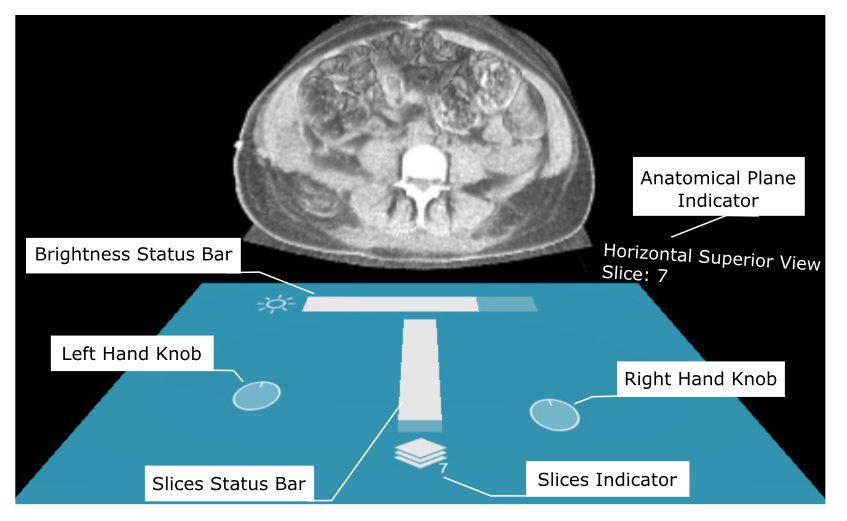
\includegraphics[width=1\textwidth]{figures/vroom_desk.png}
          \captionof{figure}{Virtual desk, control indicators, and medical images rendering in  \cite{sousaVRRRRoomVirtualReality2017}}
          \label{fig:vroom_desk}
        \end{minipage}
    \end{figure}

    The visualization of controls on a virtual desk, exemplified in VRRRRoom \cite{sousaVRRRRoomVirtualReality2017} and illustrated in Figure \ref{fig:vroom_desk}, serves as a valuable tool for instructing users about available gestures and conveying information such as the current volume slice. Zielasko et al. \cite{zielaskoNonStationaryOfficeDesk2019} conducted an experiment to assess the impact of introducing this virtual desk into the virtual environment, analyzing its effects on performance, cybersickness, and presence. Their findings indicated no significant differences in the evaluated aspects, suggesting the potential for expanding the desk functionality to incorporate menus or controls.

    Regarding the selection and manipulation of 3D objects, many techniques are viable in both standing and sitting positions. However, techniques requiring extra controllers may be less suitable, as finding them after being set down while immersed in an HMD can be difficult \cite{zielaskoRemainSeatedFullyimmersive2017}. Almeida et al. \cite{almeidaSIT6IndirectTouchbased2023} developed a DeskVR-specific object manipulation technique called SIT6. This indirect touch-based technique utilizes a gesture dictionary with separated degrees of freedom: three for translation and three for rotation, as seen in Figure \ref{fig:sota_sit6}.  Indirect touch means that users do not directly touch the object through a screen display but interact with it indirectly, as the former would not be practical in VR using an HMD \cite{mendesSurvey3DVirtual2019}. While SIT6 may not be as fast as other state-of-the-art mid-air techniques, it was found to be as effective and less physically demanding.

    \begin{figure}[h]
        \centering
        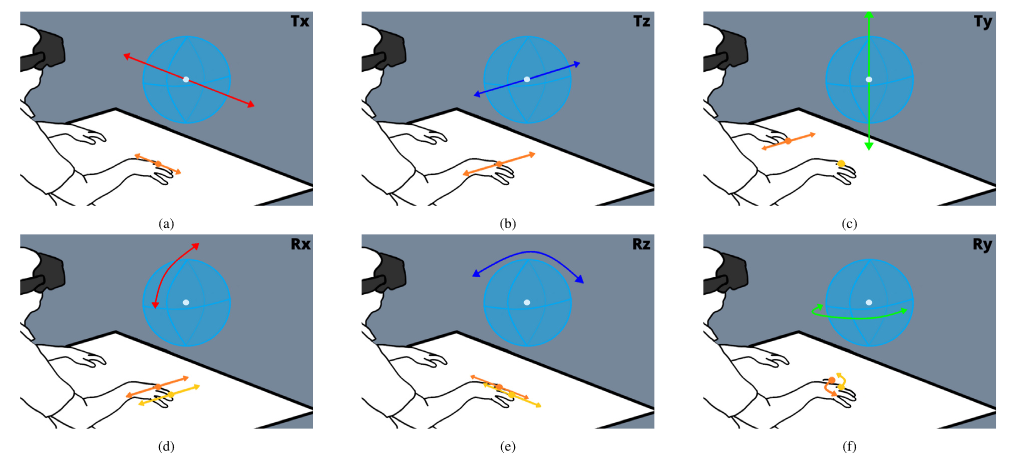
\includegraphics[width=1\linewidth]{figures/sit6.png}
        \caption{The gesture dictionary of SIT6 \cite{almeidaSIT6IndirectTouchbased2023}. Gestures (a), (b), and (c) represent translation movements, while gestures (d), (e), and (f) represent rotation movements.}
        \label{fig:sota_sit6}
    \end{figure}

    Designing traveling techniques in DeskVR is challenging because users are seated, rendering real walking impractical despite its potential presence enhancement. While presence is crucial for reducing cybersickness \cite{zielaskoRemainSeatedFullyimmersive2017}, an effective travel technique in DeskVR should aim to enhance presence without necessitating tiring motions or additional body tracking, such as leg movements. Amaro et al. \cite{amaroDesignEvaluationTravel2022} devised three travel and four orientation techniques, seen in Figure \ref{fig:sota_travel}. One travel technique utilized a VR controller named Continuous Directional Movement. In contrast, the others employed a touch surface and gestures, known as Dog Paddle and Drag'n Go.

    \begin{figure}[h!]
        \centering
        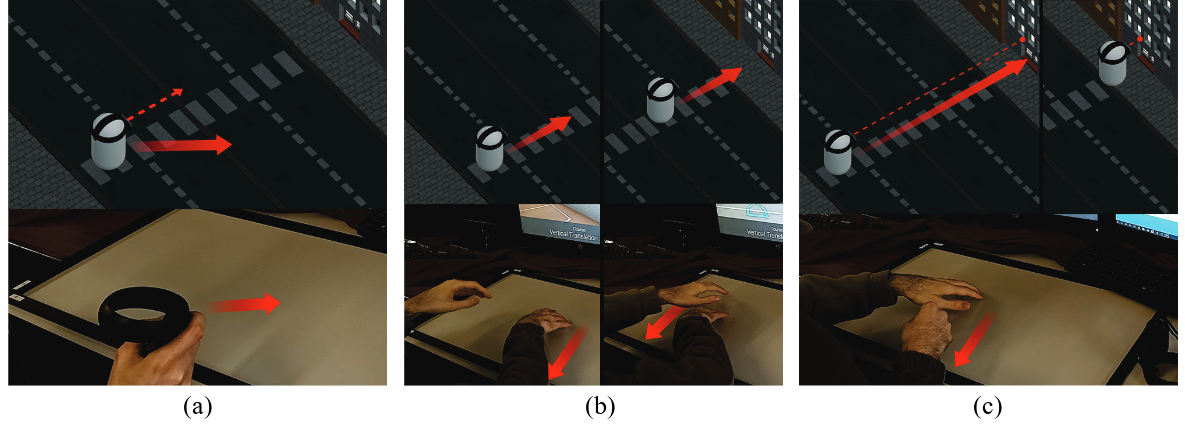
\includegraphics[width=1\textwidth]{figures/sota_travel.png}
        \captionof{figure}{Travel techniques designed for DeskVR by Amaro et al. \cite{amaroDesignEvaluationTravel2022}: Continuous Directional Movement (a), Dog Paddle (b), Drag'n Go (c).}
        \label{fig:sota_travel}
    \end{figure}

    For orientation, Amaro et al. \cite{amaroDesignEvaluationTravel2022} introduced two techniques utilizing VR controllers, named Continuous Directional Rotation and Choose \& Click, one technique utilizing a tactile surface, named Tactile Surface Dragging, and one technique relying on the orientation of the user's head, named Gaze Convergence. These techniques are illustrated in Figure \ref{fig:sota_orientation}. Among the movement techniques, Continuous Directional Movement outperformed its counterparts in performance and comfort, although it appeared to induce more nausea than Dog Paddle. The discomfort in Dog Paddle could stem from its repetitive, exaggerated motions, indicating a potential avenue for exploring more straightforward and less straining interactions. Concerning orientation, Tactile Surface Dragging exhibited superior overall performance, showing fewer cybersickness symptoms than Continuous Directional Rotation, which exhibited the most.

    \begin{figure}[h!]
        \centering
        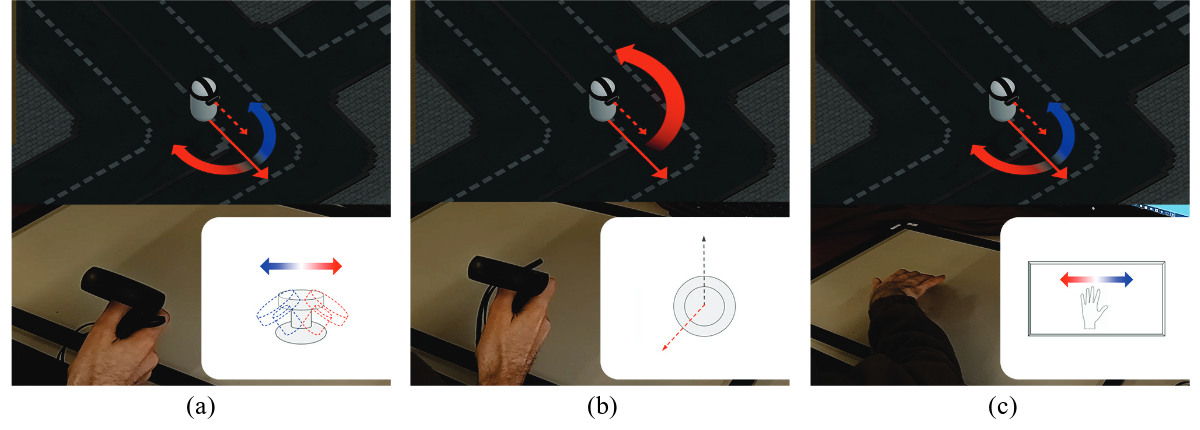
\includegraphics[width=1\textwidth]{figures/sota_orientation.png}
        \captionof{figure}{Orientation techniques designed for DeskVR by Amaro et al. \cite{amaroDesignEvaluationTravel2022}: Continuous Directional Rotation (a), Choose \& Click (b), Tactile Surface Dragging (c).}
        \label{fig:sota_orientation}
    \end{figure}


\section{Discussion} \label{sec:sota_discussion}

    The key takeaway in developing interactions for DeskVR is prioritizing user comfort and leveraging the potential benefits of having a desk in front of the user while being mindful of the associated constraints. Numerous studies have investigated the effectiveness of touch-based interactions in both non-steroscopic contexts, such as Balloon Selection \cite{benkoBalloonSelectionMultiFinger2007}, Corkscrew Selection \cite{daiberBalloonSelectionRevisited2012}, and Triangle Cursor \cite{strothoffTriangleCursorInteractions2011}, and in the context of DeskVR, exploring various scenarios such as menu navigation \cite{zielaskoMenusDeskSystem2019}, medical image data examination for radiologists \cite{sousaVRRRRoomVirtualReality2017}, travel techniques \cite{amaroDesignEvaluationTravel2022}, and object interaction \cite{almeidaSIT6IndirectTouchbased2023}. The consensus from these studies suggests that, although a touch-based approach may not always be the most time-efficient, it significantly reduces physical strain, enhancing overall comfort and prolonged usage time for individuals. This aspect is essential for DeskVR, where the primary objective is to alleviate physical strain, improve accessibility, and boost productivity \cite{zielaskoRemainSeatedFullyimmersive2017, zielaskoSitNotSit2021}. For this reason, touch-based approaches seem preferable over mid-air interactions. Furthermore, Zielasko et al. \cite{zielaskoNonStationaryOfficeDesk2019} demonstrated that presenting a virtual table as a surrogate for the physical table has minimal impact on task performance, cybersickness, and presence, making it a viable option for menus and other interactions without compromising the user experience.
    
    The absence of physical feedback during simultaneous interactions by multiple users creates unpredictability in real-time multi-user collaboration \cite{ruddleLevelsControlCollaborative2003}. While haptic devices like the Phantom Omni \cite{silvaPHANToMOMNIHaptic2009} offer a potential solution by allowing users to manipulate objects and perceive forces applied by others \cite{ruddleSymmetricAsymmetricAction2002}, their integration into DeskVR, potentially involving substitutional reality -- replacing real physical objects such as haptic devices with virtual counterparts \cite{simeoneSubstitutionalRealityUsing2015}, is beyond the scope of this work. Furthermore, the limited mobility of users in DeskVR constrains simultaneous multi-user object interaction, particularly when considering physics-based interaction techniques such as concurrency control using consensus-based networking \cite{fristonConsensusBasedNetworking2022}.

    Considering these factors, level 3 collaboration is unsuitable, and thus, there is no need for distributed average concurrency control techniques. Additionally, degree-of-freedom separation techniques appear restrictive in configuration and interaction while potentially confusing and difficult to use. As such, the fine-grained approach of Lee et al. \cite{leeSupportingFineGrainedConcurrent2012} is appealing, allowing users to discuss different object interactions and arrangements while sharing their perspectives. This approach influenced the idea of using the world-in-miniature \cite{stoakleyVirtualRealityonaWim1995} metaphor for the design of Replico, which plays to the strengths of DeskVR.

    Moreover, providing social visibility, awareness, and accountability in collaborative environments is pivotal in shaping how we communicate \cite{ericksonSocialTranslucenceApproach2000, gutwinDescriptiveFrameworkWorkspace2002}. The chosen approach should provide these elements, enabling users to communicate more effectively. For instance, it should indicate who is interacting with an object, its owner, and who is engaged in the conversation, seamlessly integrating these aspects within the DeskVR environment. Additionally, it should leverage the spatial attribute of VR, incorporating a spatial model of interactions \cite{benfordSpatialModelInteraction1993, dominguesCollaborative3DInteraction2011}. Users within the proximity of an object's aura could trigger interactions, such as audio communication, enabling them to focus on the task at hand with fewer distractions. This aligns with the concept of translucence as discussed by Erickson and Kellogg \cite{ericksonSocialTranslucenceApproach2000}.


    %\cite{odaVirtualReplicasRemote2015}
    %\cite{tianUsingVirtualReplicas2023}

\chapter{Replico}\label{chap:method}

    % todo: cite wim
    After evaluating the literature, there appears to be a promising avenue for exploring a method for DeskVR users to engage in discussions and communicate about various objects and areas of interest within a shared virtual environment. This approach could enhance communication effectiveness, especially considering the challenges associated with verbally referencing objects and describing spatial locations \cite{odaVirtualReplicasRemote2015}. Moreover, given the unique constraints of DeskVR, a research gap exists in applying such methods to this specific environment. Thus, this work introduces Replico, a collaborative touch-based DeskVR approach that utilizes the world-in-miniature (WIM) \cite{stoakleyVirtualRealityonaWim1995} metaphor to facilitate reasoning about 3D models.

\section{Overview} \label{sec:overview}

    After recognizing the potential of a collaborative DeskVR approach to enhance communication and reasoning about 3D models, it became important to outline the basic needs such an approach should meet. These requirements stem from the desire to address common challenges faced by users in virtual environments, aligning with DeskVR's goals of minimizing physical effort to enable longer periods of productive work, reducing mistakes to prevent frustration, and getting more done in less time. Additionally, the approach should be easy to understand to facilitate seamless collaboration with others and allow users to communicate effectively about objects and areas of interest even when they are out of sight.

    Furthermore, users must know where others are, who they are, and what they are doing in the virtual space to work well together. Users should be able to easily determine the location and activities of their counterparts so they can coordinate and talk effectively. Importantly, all interactions and tasks should be achievable while seated so they can keep working without getting too tired.

    To meet these needs, the chosen approach utilizes the world-in-miniature (WIM) metaphor \cite{stoakleyVirtualRealityonaWim1995}. The WIM is a miniature replica of the virtual environment that can be easily manipulated within arm's reach and viewed from multiple angles, making it a good fit for DeskVR. Changes made in the miniature model are reflected in the full-scale model. Additionally, the WIM is effective for displaying social information, such as users' locations and where they are looking, as well as indicating who is working. Each user has a personal view of the WIM, while the to-scale model is shared.

    The approach allows users to create points of interest to facilitate communication about objects and zones of interest. These points are uniquely identified by a number and an appearance corresponding to their owner. For instance, one user's points of interest might be represented by green striped spheres, while purple checkerboard cubes represent another user's points. These points of interest are visible in both the to-scale 3D model and its WIM counterpart and remain visible even if occluded.

    Users are attached to virtual tables that correspond to their real-life counterparts. They can either remain at separate tables or join another user's table to share the same point of view of the to-scale model. Users can also teleport around the 3D model, taking their table with them if they are alone or creating a new one if they are at someone else's table.

    To reduce physical effort, the approach uses touch-based gestures for interactions, such as moving the replica and creating points of interest. Literature suggests that touch-based interactions help reduce physical strain and increase comfort \cite{benkoBalloonSelectionMultiFinger2007, almeidaSIT6IndirectTouchbased2023}. Specifically, the approach incorporates the Balloon Selection metaphor \cite{benkoBalloonSelectionMultiFinger2007} for creating points of interest. Balloon Selection was chosen mainly due to its "String Height Clutching" feature, which allows users to increase the height of the selection cursor infinitely. This is in contrast to the Triangle Cursor \cite{strothoffTriangleCursorInteractions2011}, and it is less straining than Corkscrew Selection \cite{daiberBalloonSelectionRevisited2012}, which requires rotational movement.

    %\begin{figure}
    %    \centering
    %    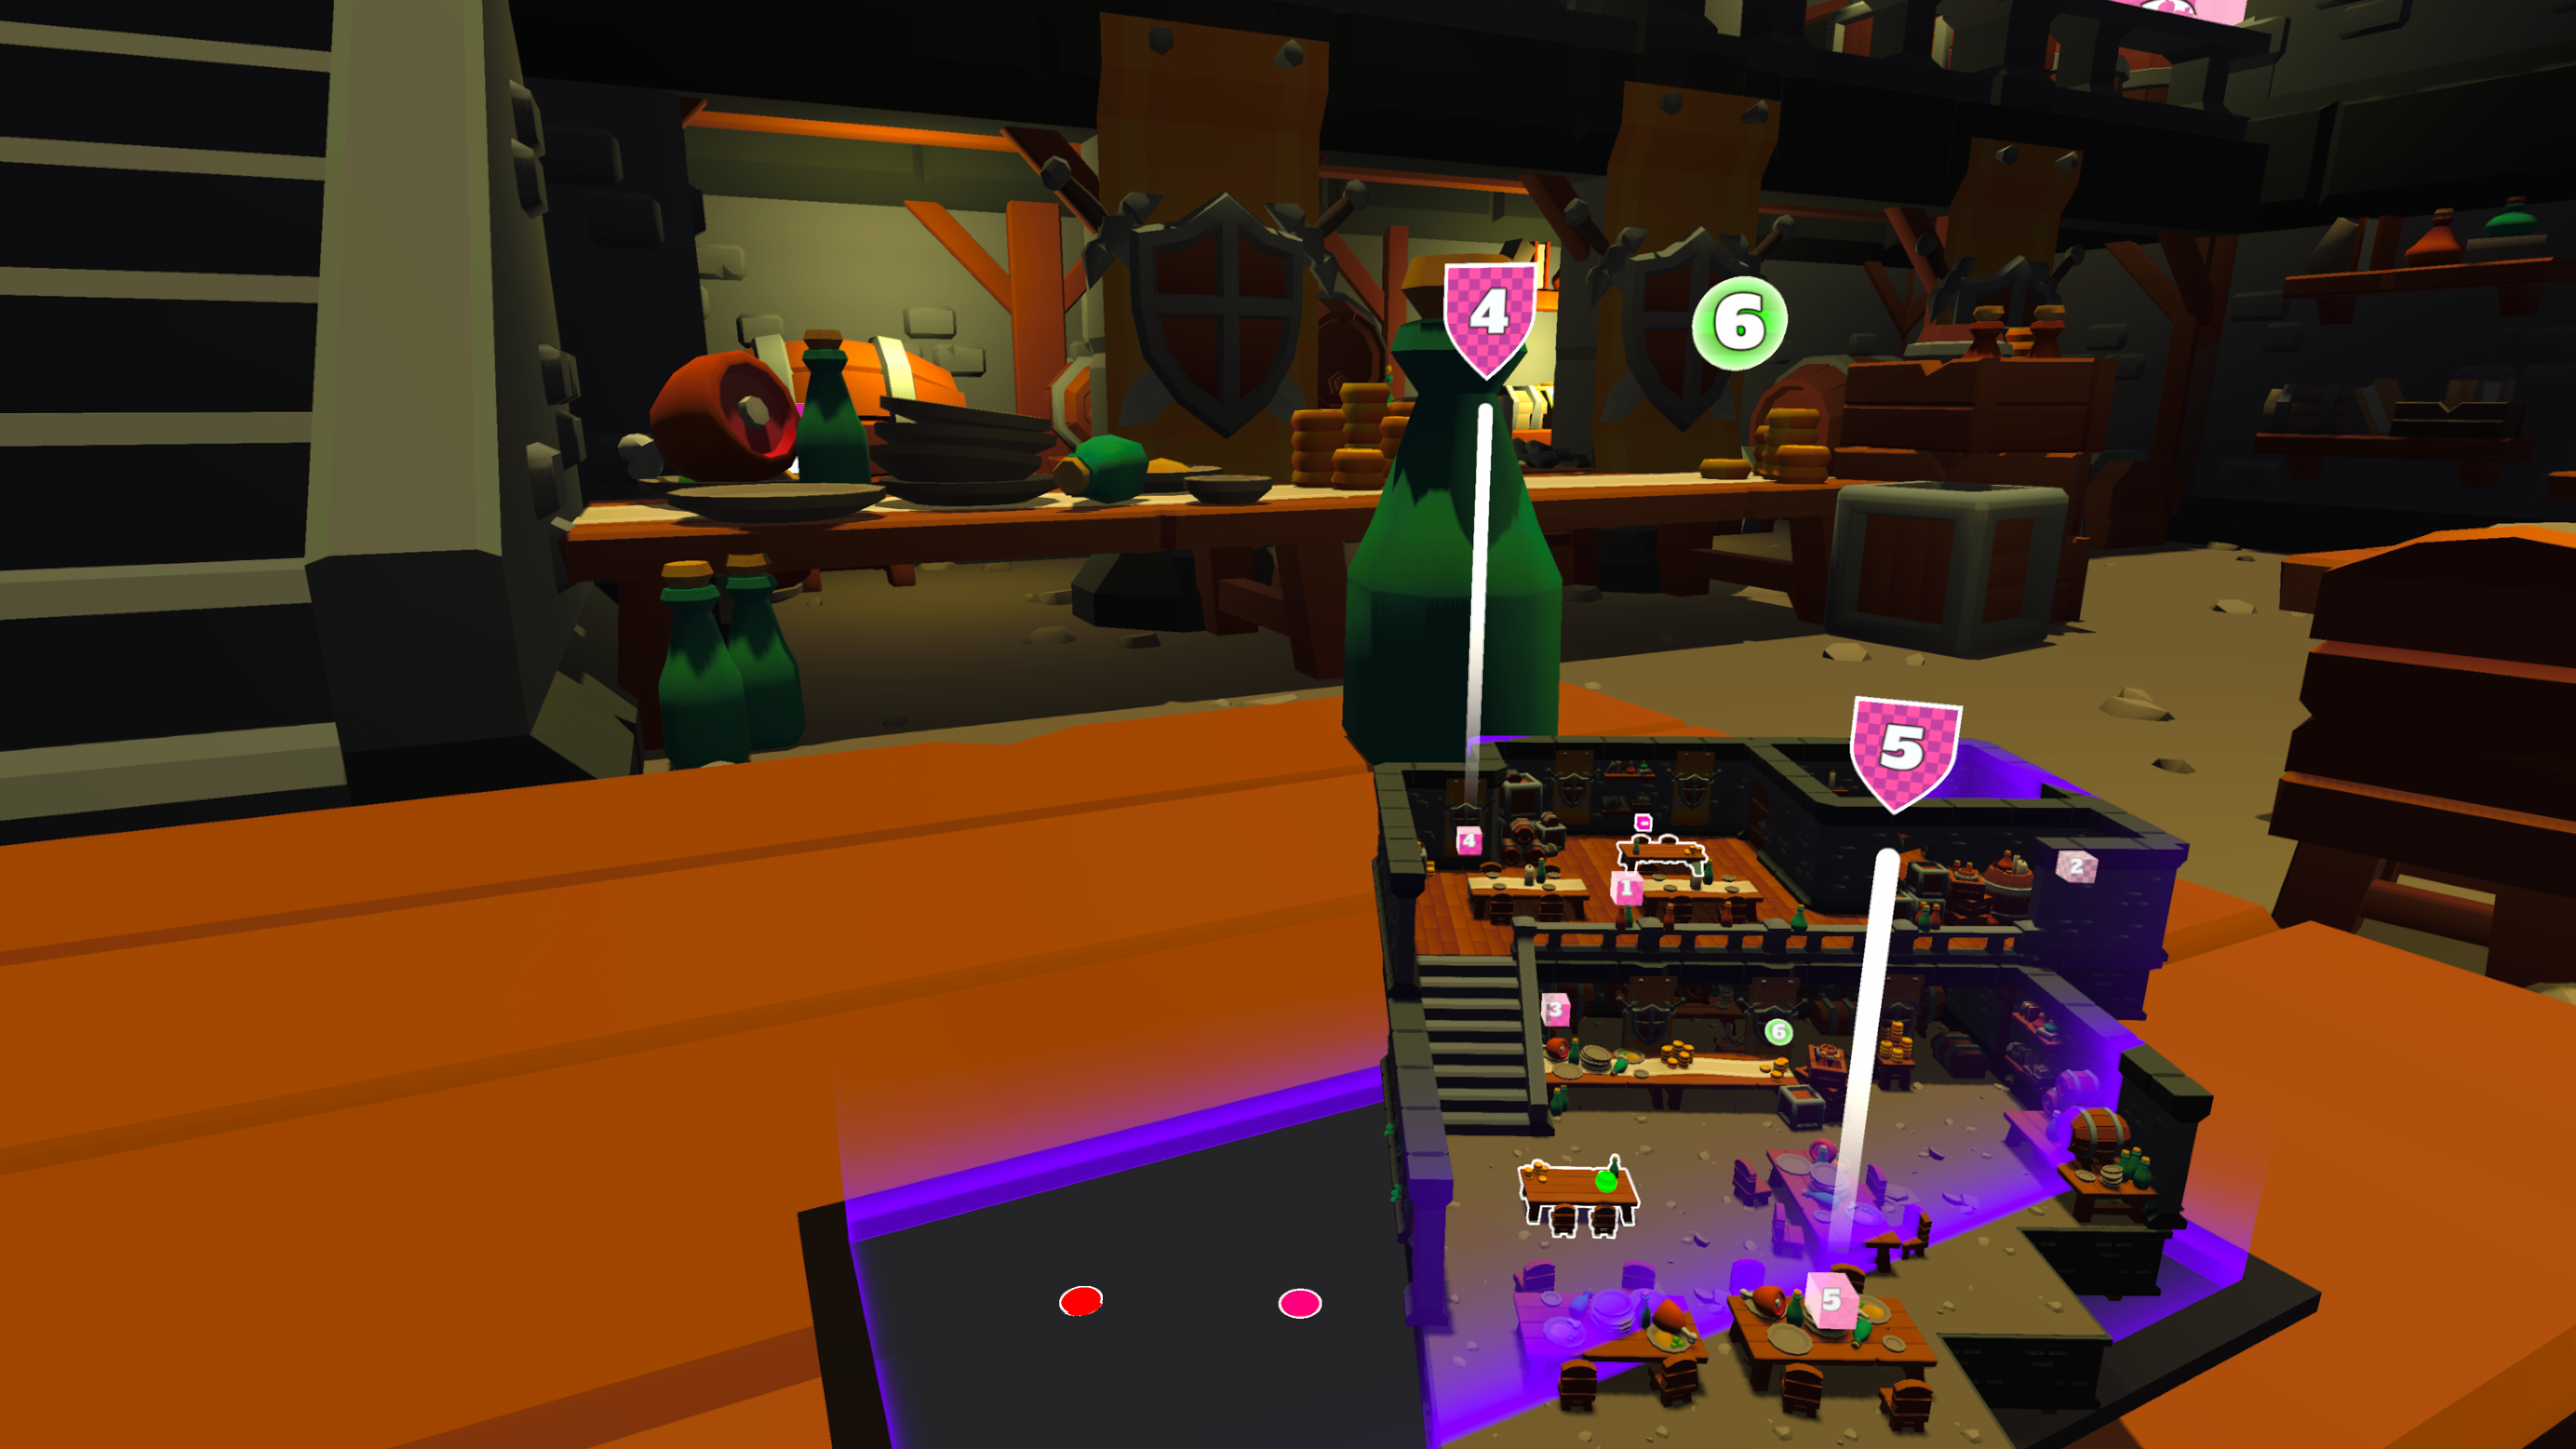
\includegraphics[width=1\linewidth]{figures/description.png}
    %    \caption{Usage example of the approach from the implemented prototype. This figure shows various elements: a virtual representation %of the user's table, a representation of the touch frame and active fingers, points of interest, and user locations.}
    %    \label{fig:description}
    %\end{figure}
    
\section{Actions} \label{sec:actions}

    This section details the specific actions users can perform within Replico using touch-based gestures. These actions encompass various interactions and transformations. Similar to Balloon Selection \cite{benkoBalloonSelectionMultiFinger2007}, these gestures are handedness-agnostic, meaning they can be performed with either the left or right hand. The following subsections outline the key actions and how to perform them.

    \subsection{Replica Transformations} \label{sec:transform}

        Transformations to the replica closely resemble the common gestures associated with touch screens on mobile phones for zooming, panning, and rotating images. Translation in the XZ plane is done by placing one or more fingers on the touch table and moving them. Yaw rotation around the Y-axis is achieved by rotating the fingers around the center of their positions, which also serves as the center of rotation. Scaling the replica in all dimensions is accomplished using a pinch gesture, with the scaling base centered on the midpoint of the fingers and the WIM's base y position.

        Translation along the Y-axis is achieved by first placing a finger from the primary hand on the table, followed by two fingers from the secondary hand. The fingers of the secondary hand control translation on the XY plane, while the fingers of the primary hand can perform all the previously mentioned transformations.

        % I have to put in here some images, not sure what

    \subsection{Balloon Selection} \label{sec:balloon}

        Replico uses the Balloon Selection metaphor \cite{benkoBalloonSelectionMultiFinger2007} to create, delete, and acknowledge points of interest, as well as teleportation, and join another user's table. To initiate the balloon selection gesture, the user places a finger from their primary hand on the table, followed by a finger from their secondary hand. This action brings up a balloon on the user's table relative to the WIM, with a copy visible on the to-scale 3D model. The primary finger controls the XZ position of the balloon while moving the fingers apart lowers the balloon, and bringing them together raises it. Users can remove the secondary finger without changing the balloon's height, allowing for "String Height Clutching."
    
        To perform a \textit{selection}, the user briefly adds a second finger from their secondary hand to the touch table. This \textit{selection} action can create points of interest at the balloon's position, delete points of interest if the balloon intersects with one of the user's points, acknowledge points of interest if the balloon intersects another user's unacknowledged points, and join other users' tables if it intersects another user's table.
    
        For \textit{teleportation}, the user similarly adds a second finger from their secondary hand to the touch table but holds it in place until an arrow appears on the balloon, indicating the teleportation's end orientation. To rotate the balloon, the user performs a gesture similar to the replica's rotation gesture by rotating their fingers around their midpoint. Either hand can be removed to reposition, but removing both hands cancels the teleportation. To confirm the teleportation, the user taps again with the second finger of the secondary hand.


\section{Awareness} \label{sec:awareness}

    Following Table \ref{tab:workspaceElementsPast}, Replico incorporates most elements of workspace awareness. Users have distinct appearances that uniquely identify them, which is also reflected in their points of interest, albeit with some distinguishing features. User tables are represented in the WIM by outlined miniatures, positioned and oriented as they are in the to-scale model, and are visible behind objects. These miniature tables display who is at each table through miniature representations of the users.
    
    Points of interest created by other users are initially in an \textit{unacknowledged} state, marked by a vertical line capped with a symbol that resembles the owner's appearance and includes the balloon's identification number. This system, combined with the acknowledgment gesture described in \ref{sec:balloon}, allows users to distinguish recently created points of interest from previously created ones.
    
    These representations blend abstract and mimetic representations of social information as described in \cite{ericksonSocialTranslucenceApproach2000}. They are mimetic in representing real-world entities like tables and user avatars, yet abstract as they are symbolic and easy to create and manipulate.
    
    Thus, Replico allows users to ascertain the presence of others in the workspace, their locations, and their viewing directions by observing the tables in the replica. Users can identify others by their appearance, determine collaborators by noting who shares the same table, and discern authorship through the appearance of points of interest. Points of interest, in turn, indicate which objects users are working on. Additionally, users can track recent activities by checking unacknowledged points.

\section{Summary}
    This chapter introduces Replico, a collaborative DeskVR approach designed to enhance communication and interaction in the analysis of 3D models. Using the world-in-miniature (WIM) metaphor, Replico addresses common challenges in virtual collaboration, such as spatial referencing and awareness of other users' activities.

    First, it explains the requirements such an approach should consider, such as minimizing physical effort, reducing mistakes, ensuring efficiency, effective communication about objects and areas of interest, ease of understanding, providing awareness of other users, and enabling all interactions to be done while seated. To meet these requirements, Replico allows users to manipulate a miniature replica of the virtual environment (WIM). This approach ensures that changes made in the miniature are reflected in the full-scale model. Replico also enables the creation of uniquely identified points of interest, aiding the communication about objects and zones of interest within the virtual space. Users are attached to virtual tables corresponding to their real-life counterparts, allowing them to join others' tables or teleport around the 3D model.

    Section \ref{sec:actions} explains the different touch-based gestures users can perform within Replico: translation, rotation, and scaling of the WIM; and creation, deletion, and acknowledgment of points of interest, as well as teleportation and joining users' tables, using balloon selection. Section \ref{sec:awareness} explains how Replico incorporates workspace awareness: users and their points of interest share a unique appearance, making them identifiable; user tables are represented in the replica; and points of interest can be acknowledged to identify recent points of interest quickly.
\chapter{Implementation of a Prototype}\label{chap:prototype}

This chapter describes the implementation of the prototype created to test the viability of Replico. It begins by explaining the architecture, hardware, software, and tools used to develop the prototype. The chapter then details how hand detection is performed, the various states within the system, how tables are tracked, how finger input is interpreted, the methods for displaying feedback to users, and the networking implementation details.

\section{Architecture}
    
    To develop the prototype, two HTC Vive Pro 2 headsets and two multi-touch surfaces -- a 32-inch infrared frame and a 47-inch capacitive Displax Skin Ultra\footnote{\url{https://www.displax.com/skin-ultra} } touchscreen -- were used. The Unity\footnote{\url{https://unity.com/}} game engine was chosen for its robust VR support, personal previous experience, extensive community resources, and excellent compatibility with external C\# libraries, which helped reduce development risks.
    
    Unity's OpenXR plugin\footnote{\url{https://docs.unity3d.com/Packages/com.unity.xr.openxr@1.11/manual/index.html}} controls VR hardware communication, handling input and rendering with minimal effort, and managing all API calls automatically. OpenXR\footnote{\url{https://registry.khronos.org/OpenXR/specs/1.1/html/xrspec.html}} is an API standard developed by Khronos for XR applications, including VR, and is widely adopted across many XR devices with conformant runtimes. Due to its ubiquity and recency, it was chosen over alternatives such as using SteamVR directly.

    Since Unity's OpenXR plugin interfaces with Unity's Input System, the Unity Enhanced Touch API\footnote{\url{https://docs.unity3d.com/Packages/com.unity.inputsystem@1.0/api/UnityEngine.InputSystem.EnhancedTouch.html}} was used instead of the standard Unity Touch API to maintain a consistent input management system. The Enhanced Touch API provides automatic finger tracking and keeps a history of touch interactions.

    The first-party Unity Netcode for GameObjects\footnote{\url{https://docs-multiplayer.unity3d.com/netcode/current/about/}} library was used for networking. This library offers a straightforward abstraction of networking logic and is easy to use and set up for client-server or distributed authority topologies. Its simplicity is well-suited for a small number of clients, making it ideal for this prototype.


    \begin{figure}[h]
        \centering
        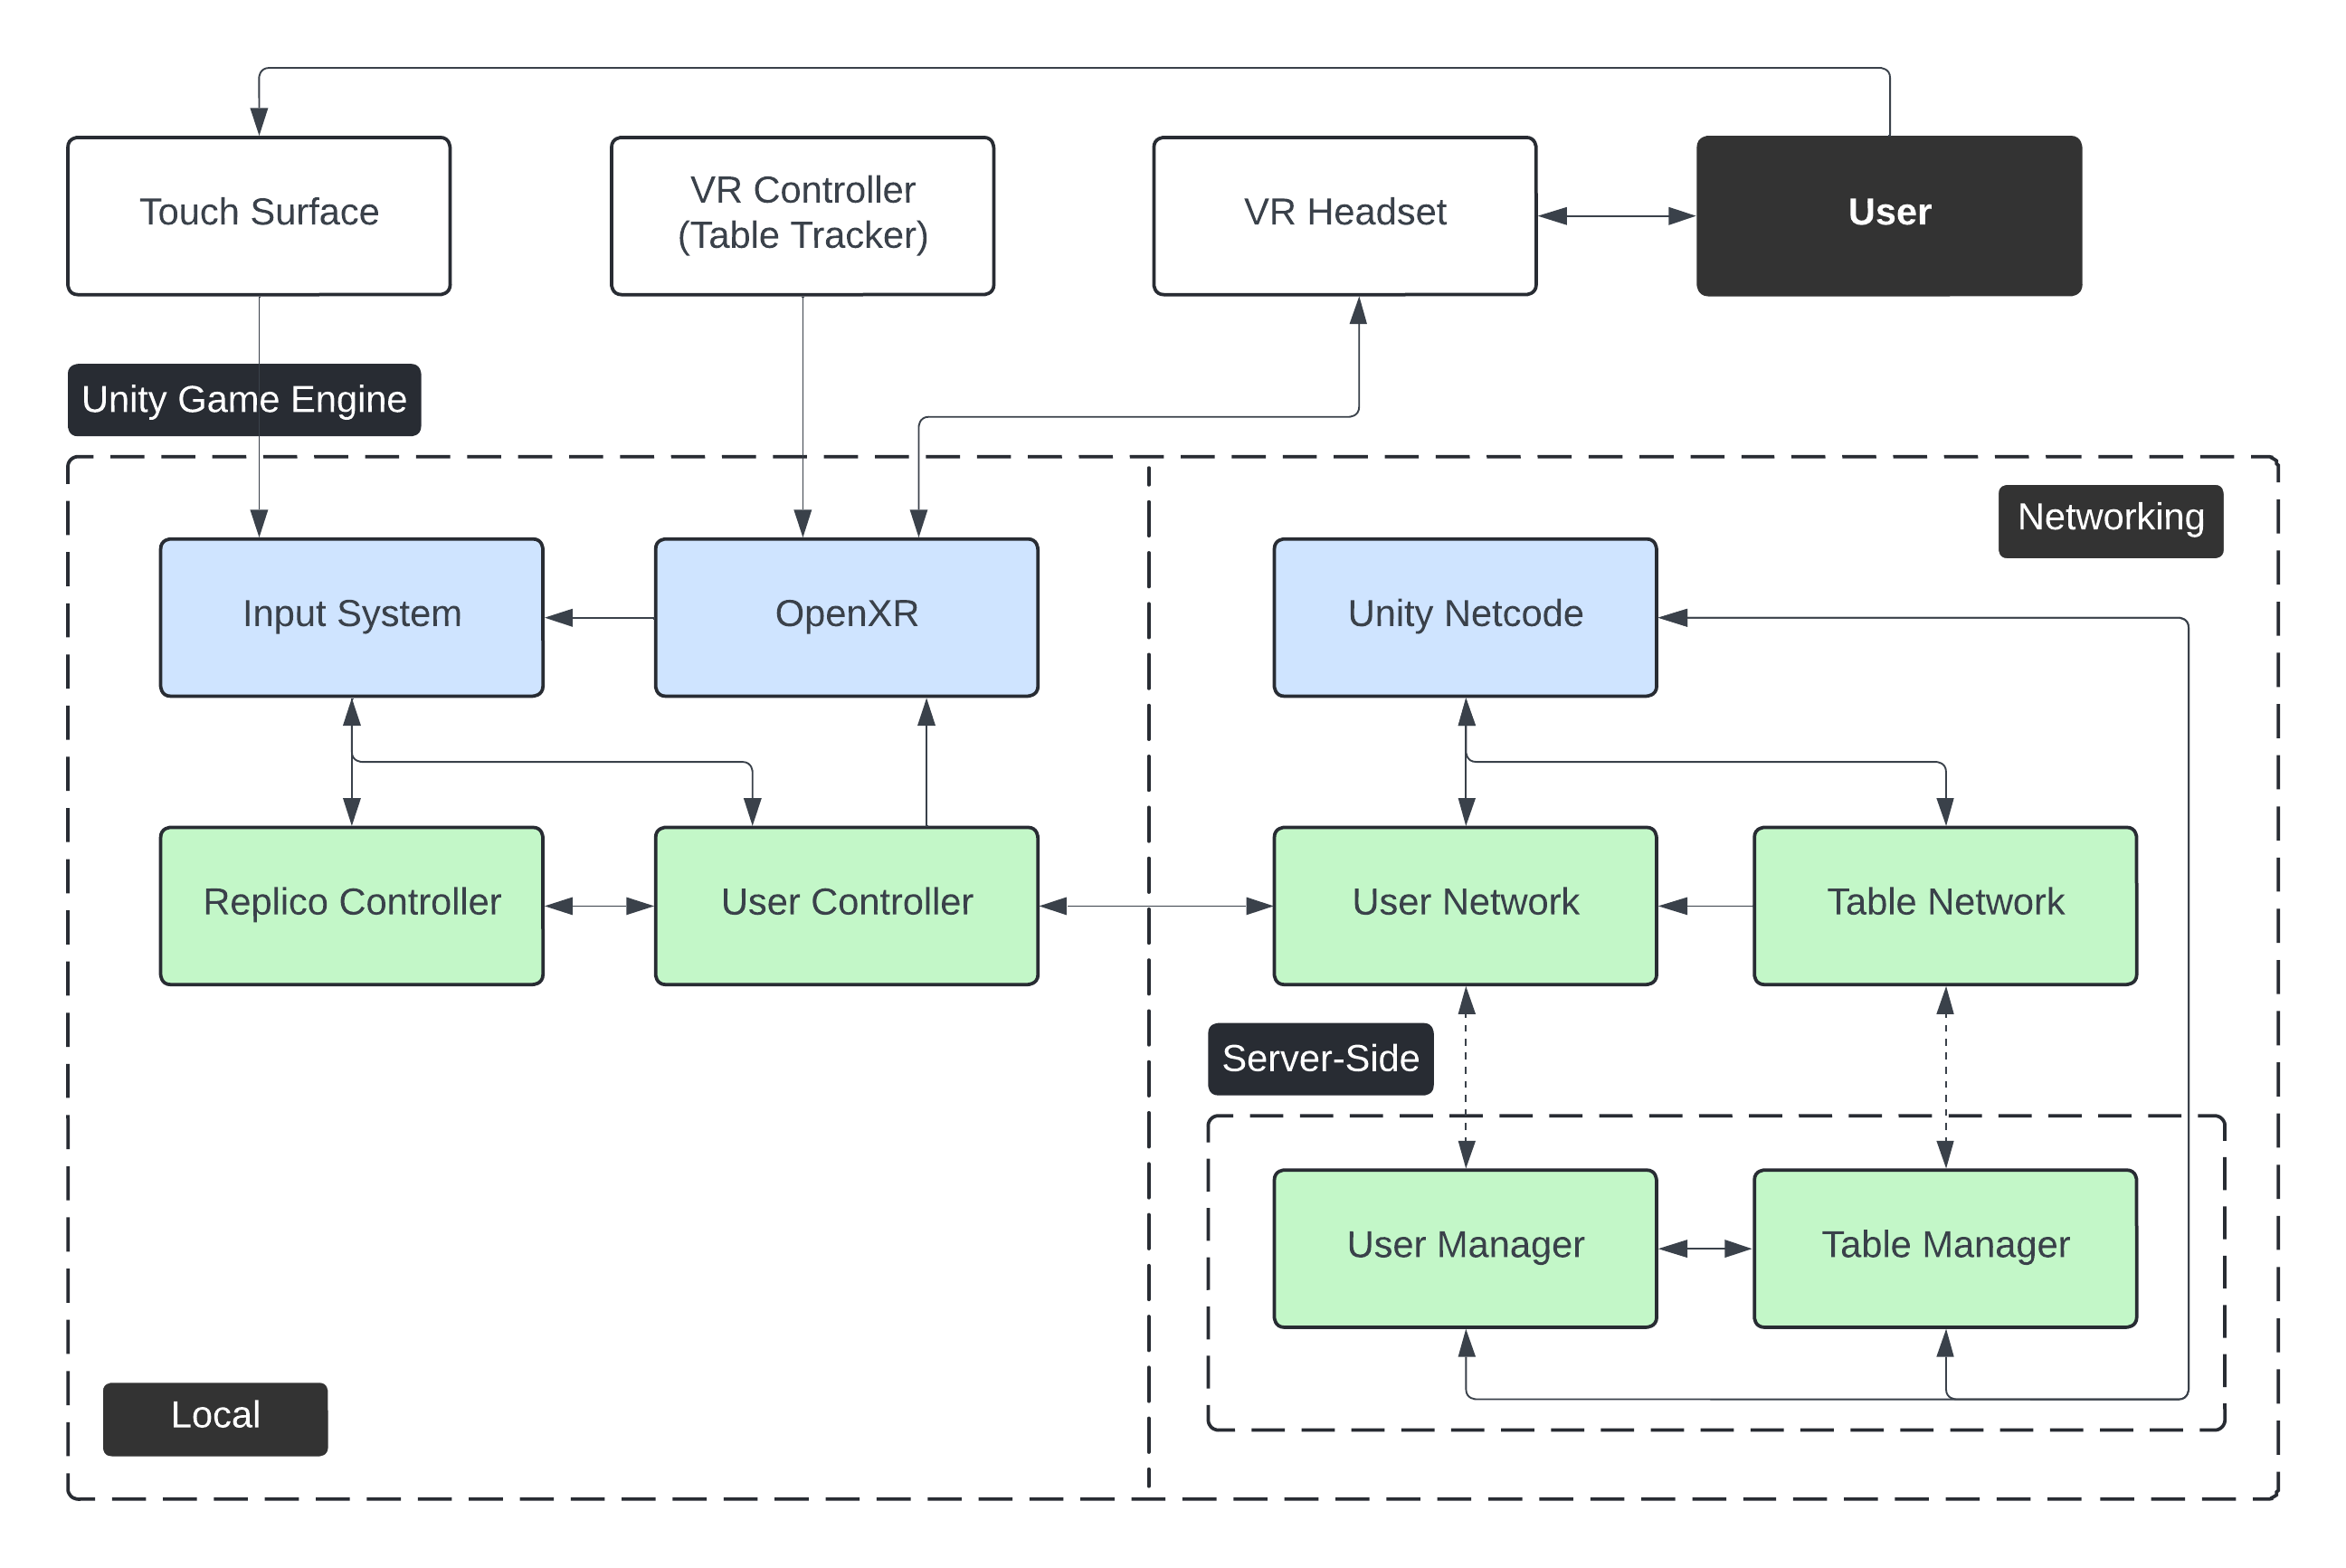
\includegraphics[width=.97\linewidth]{figures/architecture.png}
        \caption{System architecture. Modules in blue represent Unity libraries, while the prototype implements modules in green.}
        \label{fig:architecture}
    \end{figure}
    
    The system architecture diagram in Figure \ref{fig:architecture} demonstrates the integration of various software and hardware components, describing both local and networked elements. OpenXR manages communication with the VR headset and the table tracker, rendering images to the headset, updating the virtual camera's position, and interfacing inputs to Unity's Input System. Unity's Enhanced Touch API processes touches sensed by the touch surface. The Replico Controller and User Controller manage interaction logic and user actions, communicating with the Input System and OpenXR. Networking is handled by Unity Netcode, which synchronizes user and table data across the network via the User Network and Table Network, using a client-server topology. The server-side User Manager and Table Manager manage data for users and tables. The User Manager tracks users in the system and communicates with the User Network objects through remote procedure calls (RPCs) and network variables. The Table Manager handles table creation, deletion, and management logic, communicating with Table Network objects using RPCs and network variables.


        % city
        % rover and ground textures
        % dungeon assets and the modular asset builder tool (https://fertile-soil-productions.itch.io/mast)

\section{State Machine}

    The interpretation of touch surface input varies depending on the gestures employed. To address this, a state machine was created. A state machine consists of defined states with distinct transitions, where each state processes the input differently. The implementation was done through the state design pattern, wherein each step is represented as a class that alters the behavior of the Replico controller. Figure \ref{fig:states} provides a diagram illustrating the implemented state machine.

    \begin{figure}[h]
        \centering
        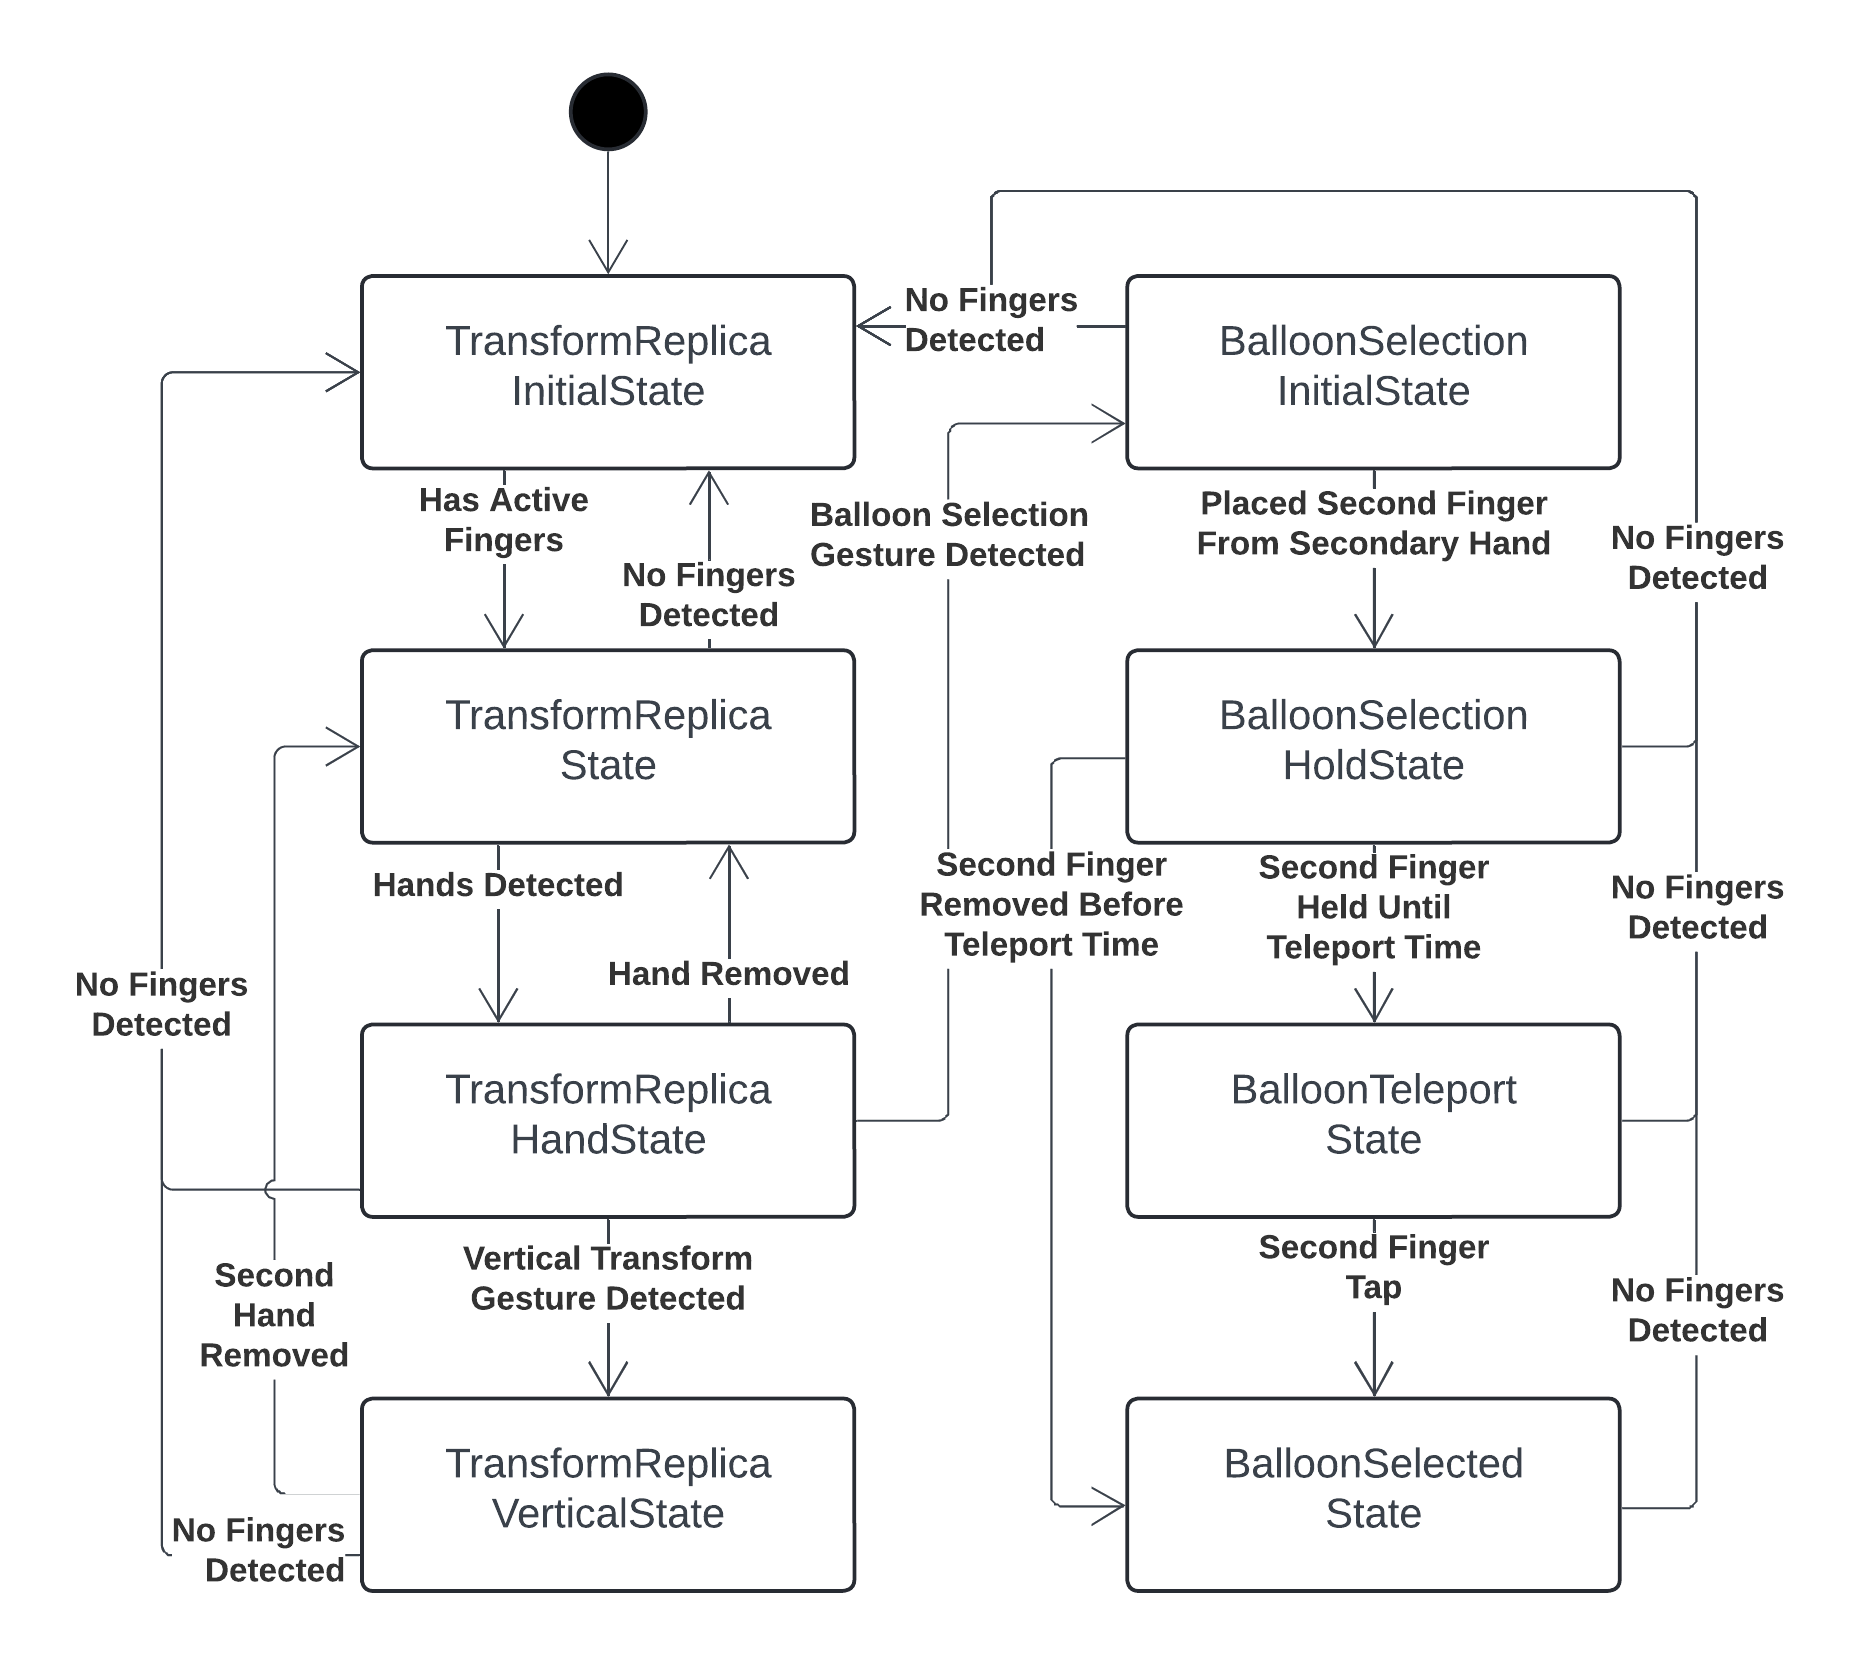
\includegraphics[width=1\linewidth]{figures/states.png}
        \caption{State machine diagram.}
        \label{fig:states}
    \end{figure}

    The \lstinline{TransformReplicaInitialState} is the starting state where no fingers are detected, and therefore no controls are active. In this state, finger touches are checked every frame using the Enhanced Touch API, which updates every frame because the Input System update mode is set to Dynamic. When at least one finger is detected, the system transitions to \lstinline{TransformReplicaState}. All states revert to this initial state whenever no fingers are detected.
    
    The \lstinline{TransformReplicaState} is entered when fingers are detected, but no hands are recognized yet. In this state, the user can move the replica using the gestures described in Section \ref{sec:transform} and implemented in Section \ref{sec:transformation}. This state performs hand detetction using the method described in Section \ref{sec:hand}, every frame. When both hands are detected, it transitions to \lstinline{TransformReplicaHand}\lstinline{State}.
    
    In \lstinline{TransformReplicaHandState}, users can move the replica as in \lstinline{TransformReplica}\lstinline{State}. This state checks what gesture the user is doing in every frame using the method described in Section \ref{sec:vertical_balloon}. It transitions to \lstinline{TransformReplicaVerticalState} if the vertical transform gesture is detected, or to \lstinline{BalloonSelectionInitialState} if the balloon selection gesture is detected. If any hand is removed, it transitions back to \lstinline{TransformReplicaState}.

    In \lstinline{TransformReplicaVerticalState}, the user can move the replica as in \lstinline{TransformReplica}\lstinline{State} using their primary hand, while the secondary hand performs translation on the XY plane. To allow users to temporarily remove the secondary hand to reposition their fingers without terminating the gesture, the secondary hand may be removed for up to $0.55$ seconds before the controller transitions back to \lstinline{TransformReplicaState}.

    In \lstinline{BalloonSelectionInitialState}, the user performs the balloon selection gesture as described in Section \ref{sec:balloon}. The primary finger moves the balloon on the XZ plane, while moving the fingers together raises the balloon and moving them apart lowers it. The balloon's height is saved between gestures, so the user doesn't have to raise it each time they start balloon selection. It transitions to \lstinline{BalloonSelectionHoldState} when a second finger is added to the secondary hand. Instead of transitioning instantly to the initial state when no fingers are detected, there is a grace period of $0.15$ seconds. This grace period accounts for potential hardware tracking failures that could prematurely stop the balloon selection gesture, potentially causing frustration.

    The \lstinline{BalloonSelectionHoldState} monitors how long the user holds down the second finger from the secondary hand. If the finger is held for $0.4$ seconds or the primary hand moves, the state transitions to \lstinline{BalloonTeleportState}. Removing the finger before $0.4$ seconds results in different actions: joining a table if the balloon intersects one, acknowledging or deleting a point of interest if it intersects one, or creating a new point of interest if it intersects none, thereby transitioning to \lstinline{BalloonSelectedState}.

    In \lstinline{BalloonTeleportState}, the user can rotate their balloon using the same gesture as rotating the replica, following the calculations described in \ref{sec:transformation}. Confirmation of teleportation occurs if the user taps with the second finger of their second hand (removing and placing it again) or if two touches are detected within the hand detection distance outlined in \ref{sec:hand}. Upon confirmation, the controller transitions to \lstinline{BalloonSelectedState}.
    
    The purpose of \lstinline{BalloonSelectedState} is to act as a buffer between balloon selection interactions and replica transformations. Users can only perform replica transformations after removing all finger touches, at which point the controller transitions back to \lstinline{TransformReplicaInitial}\lstinline{State}.


\section{Replica Transformations} \label{sec:transformation}

    This section discusses the transformations applied to the replica in states \lstinline{TransformReplicaState}, \lstinline{TransformReplicaHandState}, and \lstinline{TransformReplicaVerticalState}.
    
    Translation is achieved by calculating the distance \(\vec{D} = C_{i} - C_{i-1}\), where \(C_{i}\) and \(C_{i-1}\) are the centers of the active touches on the touch surface from the current frame and the previous frame, respectively, as shown in Equation \ref{eq:center}.

    \begin{figure}[h]
    \begin{equation}
    \begin{split} \label{eq:center}
        \mathbf{F}_i &= \{(x_{i_k}, y_{i_k}) :\ k = 1,\ \dots,\ n\} \\
        \mathbf{minF}_i &= (\min_{k} x_{i_k},\ \min_{k} y_{i_k}) \\
        \mathbf{maxF}_i &= (\max_{k} x_{i_k},\ \max_{k} y_{i_k}) \\
        C_i &= \frac{\mathbf{minF}_i + \mathbf{maxF}_i}{2}
    \end{split}
    \end{equation}
    \end{figure}

    Here, \(\mathbf{F}_i\) represents the positions of the \(n\) fingers in the \(i\)-th frame, \(\mathbf{minF}_i\) and \(\mathbf{maxF}_i\) are the minimum and maximum x and y coordinates from the set of finger positions. Essentially, \(C_i\) is the geometric centroid of the smallest rectangle that can enclose all the touch points. The distance $\vec{D}$ is then multiplied by a factor \(t\), which can be adjusted for each 3D model, resulting in \(\vec{T} = t \cdot \vec{D}\). This yields a 2D vector that is added to the replica's position in the \(XZ\) plane.

    Scaling is achieved by first calculating $s = {{\left(\bar{d_i} / \bar{d_{i-1}}\right)}^{c}}$, where \(\bar{d_i}\) and \(\bar{d_{i-1}}\) are the average distances of the active touches to the center of those touches from the current frame and the previous frame, respectively, and \(c\) is a constant used to modulate the scaling effect. The calculation for the average distance is shown in Equation \ref{eq:distance}.
    
    \begin{figure}[h]
    \begin{equation}
    \begin{split} \label{eq:distance}
        \bar{d_i} &= \frac{\sum_{k = 1}^{n} \| C_i - F_{i_k} \|}{n}
    \end{split}
    \end{equation}
    \end{figure}
    
    Finally, this scaling is applied to the replica around a base point, based on the center of the fingers. To do this, the pivot point in world coordinates, \(\mathrm{pivot}_w\), is first converted to local coordinates, \(\mathrm{pivot}_l\), relative to the replica. The replica's local scale is then multiplied by \(s\). After scaling, the position of the pivot in world coordinates, \(\mathrm{pivot}_k\), calculated by converting \(\mathrm{pivot}_l\) back to world coordinates, will not be equal to \(\mathrm{pivot}_w\). To correct this, the displacement \(\vec{\Delta \mathrm{pivot}} = \mathrm{pivot}_w - \mathrm{pivot}_k\) is calculated and added to the replica's world position.

    Rotation is achieved by calculating the fingers' average rotation \(\bar{\theta}\). The calculation for this is shown in Equation \ref{eq:rotation}, where \(\vec{\mathrm{dir}_{i_k}}\) is the vector direction from the center of the fingers to the \(k\)-th finger in the \(i\)-th frame, \(|\theta_k|\) is the angle between the vector direction of the previous frame and the current frame for the \(k\)-th finger. The angle \(\theta_k\) is determined by adjusting \(|\theta_k|\) based on the cross product's \(z\)-component to account for direction, as the arccosine function's range only goes from \(0\) to \(\pi\). The replica is then rotated around the \(Y\) axis that passes through \((C_{i_x}, 0, C_{i_y})\) with the angle $\bar{\theta}$, using Unity's \lstinline{RotateAround}.

    \begin{equation}
    \begin{split} \label{eq:rotation}
        \vec{\mathrm{dir}_{i_k}} &= \mathbf{F}_{i_k} - C_i \\
        |\theta_k| &= \cos^{-1} \left( \frac{\vec{\mathrm{dir}_{{i-1}_k}} \cdot \vec{\mathrm{dir}_{i_k}}}{\|\vec{\mathrm{dir}_{{i-1}_k}}\| \|\vec{\mathrm{dir}_{i_k}}\|} \right) \\
        \theta_k &= \begin{cases} 
            |\theta_k| & \text{if} \quad (\vec{\mathrm{dir}_{{i-1}_k}} \times \vec{\mathrm{dir}_{i_k}})_z < 0 \\
            -|\theta_k| & \text{if} \quad (\vec{\mathrm{dir}_{{i-1}_k}} \times \vec{\mathrm{dir}_{i_k}})_z \geq 0
        \end{cases} \\
        \bar{\theta} &= \frac{\sum_{k=1}^{n} \theta_k}{n}
    \end{split}
    \end{equation}


    In the \lstinline{TransformReplicaVerticalState}, the primary hand can perform $XZ$ translation, rotation, and scaling, while the secondary hand can only perform translation on the $XY$ plane. Only the fingers from the primary hand are considered for transformations with the primary hand. The secondary hand's fingers can only perform translation as previously described, but instead of \(\vec{T}\) being applied to the replica's $XZ$ position, it is applied to the $XY$ position.
    
    The transformations are not directly applied to the replica; instead, they are applied to a target object. The replica then follows this target object using Unity's \lstinline{SmoothDamp} for position and scale, and \lstinline{SmoothDampAngle} for each Euler rotation angle. This helps to reduce jitter caused by low-frequency or low-accuracy touch input updates.

\section{Gesture Detection}

    This section explains how the different gestures -- transformation, vertical transformation, and balloon selection -- are distinguished. Section \ref{sec:hand} explains the method for detecting and distinguishing the user's hands, and Section \ref{sec:vertical_balloon} describes how the vertical transform and balloon selection gestures are differentiated.

    \subsection{Hand Detection} \label{sec:hand}

        Detection and distinction of hands are important for recognizing Replico's touch-based gestures. The prototype took a simplistic approach to hand detection, using input solely from the touch surface and Unity's Enhanced Touch API. The method involves detecting two clusters based on finger proximity. For this purpose, this prototype uses a naive K-Means clustering algorithm \cite{zbMATH03340881, lloydLeastSquaresQuantization1982, 1571980074621944832} with a $k$ value of $2$. The algorithm was implemented using the ML.NET library\footnote{\url{https://github.com/dotnet/machinelearning}}, a machine learning library for .NET. For compatibility with Unity, the .NET Standard 2.1 version was used. The distance function used is the Euclidean distance between the finger positions on the touch surface in pixels, 
        and the Yinyang initialization algorithm \cite{pmlr-v37-ding15} is applied.
    
        Other clustering algorithms, such as DBSCAN \cite{ester1996density}, were not used because they do not allow the specification of a fixed number of clusters ($k$) or because they perform better with a larger number of clusters. K-means is perfectly adequate in this case with a maximum of $10$ points (one for each finger) and only $2$ clusters.
    
        The K-means algorithm returns two clusters of fingers when more than one finger is placed on the touch surface. However, this can result in two fingers from the same hand being detected as separate clusters. To address this, a distance threshold between cluster centroids is used to determine if the clusters represent separate hands. The threshold distance is measured relative to a min-max normalized value of the screen dimensions in pixels. A distance threshold of $0.18$ was found to be effective through testing.
    
        Initially, before any hands have been detected in the \lstinline{TransformReplicaState} shown in Figure \ref{fig:states}, the distinction between the primary and secondary hands is maintained by queuing fingers based on the order of their touch. The cluster containing the first detected finger represents the primary hand. Once both hands are detected in the \lstinline{TransformReplicaHandState} and beyond, hands are updated each frame by reapplying the K-means algorithm. The distinction is then made by counting how many fingers from the previously detected primary hand are in each newly detected cluster; the cluster with the most fingers from the primary hand is associated with it. To update the hands, new fingers in the clusters are added to the corresponding hands, and previously detected fingers remain in their respective hands unless they have been removed from the touch surface. This approach allows left-handed and right-handed users to perform all Replico gestures easily.

    \subsection{Distinguishing Vertical Transform and Balloon Selection} \label{sec:vertical_balloon}
    
        The vertical transform and balloon selection gestures, described in Sections \ref{sec:transform} and \ref{sec:balloon} respectively, can be easily confused with the pinch gesture required for scaling the replica. To aid in this distinction:
    
        \begin{itemize}
            \item \textbf{Vertical Transform:} At least one finger on the primary hand and at least two fingers on the secondary hand. The secondary hand must remain stationary for $0.2$ seconds.
            \item \textbf{Balloon Selection:} Exactly one finger on the primary hand and exactly one finger on the secondary hand. Both hands must remain stationary for $0.2$ seconds.
        \end{itemize}
    
        The vertical transform only checks if the second hand has moved, allowing the user to add the secondary hand while transforming with the first. The criterion for determining if a hand hasn't moved is that none of its fingers have moved past a threshold $\delta$ from the position where they were first placed. This threshold is measured relative to a min-max normalized value of the screen dimensions in pixels, with testing indicating $0.01$ as an appropriate value. Once a finger has moved, it will be considered moved until it is removed.

\section{Table Tracking} \label{sec:table_tracking}

    The user's table is tracked to a real-world table using a VR controller, as shown in Figure \ref{fig:table_tracking}. The controller is positioned pointing toward the user instead of forward from the table so that the tracked controller position matches the table's corner. If it pointed the other way, a translation based on the controller's length toward the table corner would be necessary, which is not feasible for all controller types.

    \begin{figure}[h]
        \centering
        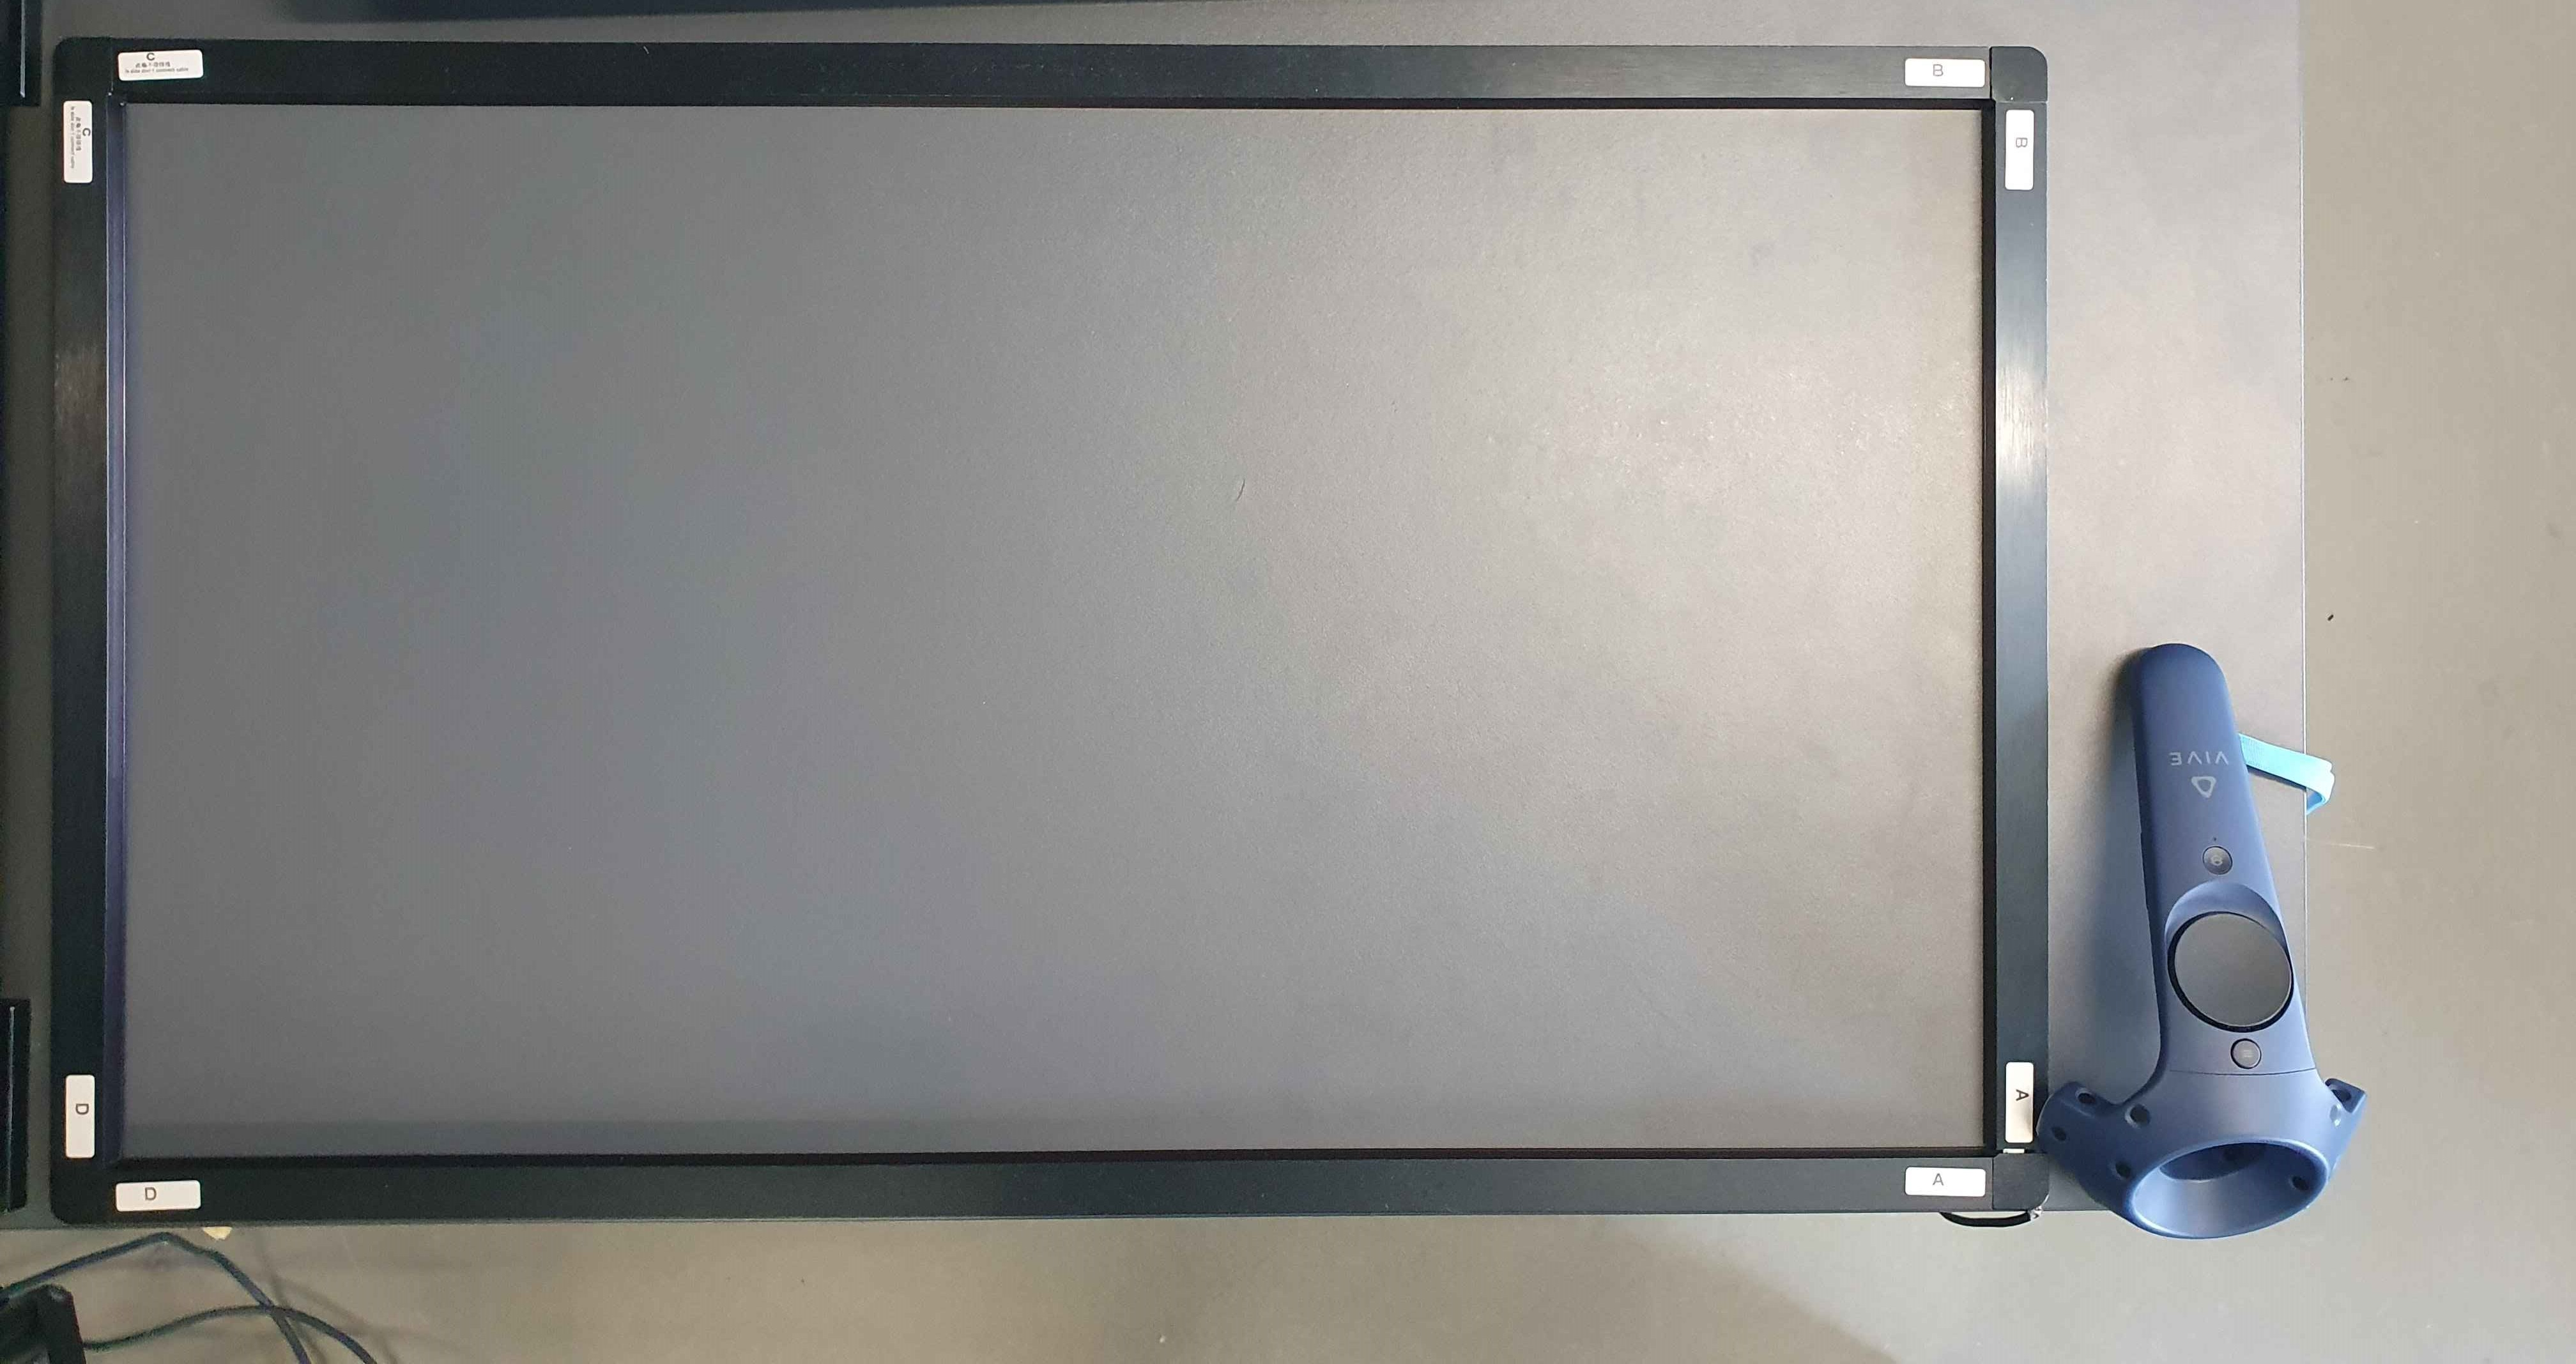
\includegraphics[width=1\textwidth]{figures/table_tracking.jpg}
        \captionof{figure}{Tracking the table using a VR controller.}
        \label{fig:table_tracking}
    \end{figure}

    When attaching a user to a virtual table, such as when the user joins a table or teleports, the orientation and position of the tracker must match the orientation and position of the table's attach point, which is an empty GameObject on the table's Prefab. To achieve this, the user's orientation is first updated using \lstinline{MatchOriginUpCameraForward}, followed by updating the position with \lstinline{MoveCameraToWorldLocation}, both functions from the OpenXR plugin. 

    The \lstinline{MatchOriginUpCameraForward} function requires two parameters: an up vector and a forward vector. The up vector is set to match the attach point's up vector, assuming the user and controller are on flat ground. The forward vector, \(\vec{v}_{\mathrm{forward}}\), is calculated as shown in Equation \ref{eq:tracker}. Here, $\mathbf{q}_{\mathrm{tracker}}$ represents the quaternion rotation of the tracker, and $\mathbf{q}_{\mathrm{attach}}$ represents the quaternion rotation of the table's attach point. $\Delta\theta$ is the rotation of the attach point relative to the tracker. The yaw component is isolated to ignore pitch and roll, preventing rotation along the x and z axes due to the controller rolling, assuming the user is on flat ground. $\mathbf{q}_{\mathrm{target}}$ is the user's target rotation, combining the user's current yaw rotation with the relative rotation of the attachment point. Finally, the forward vector is obtained by multiplying $\mathbf{q}_{\mathrm{target}}$ by the (0,0,1) vector. The \lstinline{MoveCameraToWorldLocation} function requires a position parameter. This position is calculated using the equation $P = P_{\mathrm{attach}} + P_{\mathrm{user}} - P_{\mathrm{tracker}}$.

    \begin{figure}[h]
    \begin{equation}
    \begin{split} \label{eq:tracker}
        \Delta\theta&=\mathbf{q}_{\mathrm{tracker}}^{-1}\cdot \mathbf{q}_{\mathrm{attach}} \\
        \Delta\theta_Y &= \mathrm{Quat}\left(0, \mathrm{yaw}(\Delta\theta), 0\right) \\
        \mathbf{q}_{\mathrm{user}_Y} &= \mathrm{Quat}(0, \mathrm{yaw}(\mathbf{q}_{\mathrm{user}}), 0) \\
        \mathbf{q}_{\mathrm{target}} &= \mathbf{q}_{\mathrm{user}_Y} \cdot \Delta\theta_Y \\
        \vec{v}_{\mathrm{forward}} &= \mathbf{q}_{\mathrm{target}} \cdot (0,0,1)
    \end{split}
    \end{equation}
    \end{figure}

    Because the controller may fall accidentally while the user is interacting with the touch surface and cannot see it when using the VR headset, it is only used to track the table when the user first joins a table. To achieve this, the tracker's rotation relative to the user is calculated using $\mathbf{q}_{\mathrm{local}} = \mathbf{q}_{\mathrm{tracker}} \cdot \mathbf{q}_{\mathrm{user}}^{-1}$ and stored. Additionally, the tracker's local position relative to the user is calculated using the user's \lstinline{InverseTransformPoint} function and stored.

    To convert the local rotation back to world rotation, the calculation  $\mathbf{q}_{\mathrm{tracker}} = \mathbf{q}_{\mathrm{user}} \cdot \mathbf{q}_{\mathrm{local}}$ is used. Similarly, the local position is converted back to world position utilizing the user's \lstinline{TransformPoint} function. These world coordinates and rotations are then used in the previously described calculations.

\section{Visual Feedback}

    The prototype uses various visual indicators as forms of feedback. These include a virtual touch frame with finger indicators described in Section \ref{sec:touch_frame}, a visual representation of the touch frame limits detailed in Section \ref{sec:frame_limits}, tables and points of interest visible in both the 3D model and the replica as described in Sections \ref{sec:virtual_table} and \ref{sec:visual_poi}, and effects related to balloon selection in Section \ref{sec:visual_balloon}, among others.

    \subsection{Virtual Touch Frame} \label{sec:touch_frame}

        In VR, users cannot see their hands or where their fingers are positioned. The prototype includes finger indicators within the virtual touch frame to address this issue, as depicted in Figure \ref{fig:touch_indicators}. Each finger is assigned a distinct color based on the order in which it was placed on the frame. Additionally, the finger trail shrinks from the current finger positions to previous positions, helping users understand their finger movements over time.
      
        \begin{figure}[h!]
            \centering
            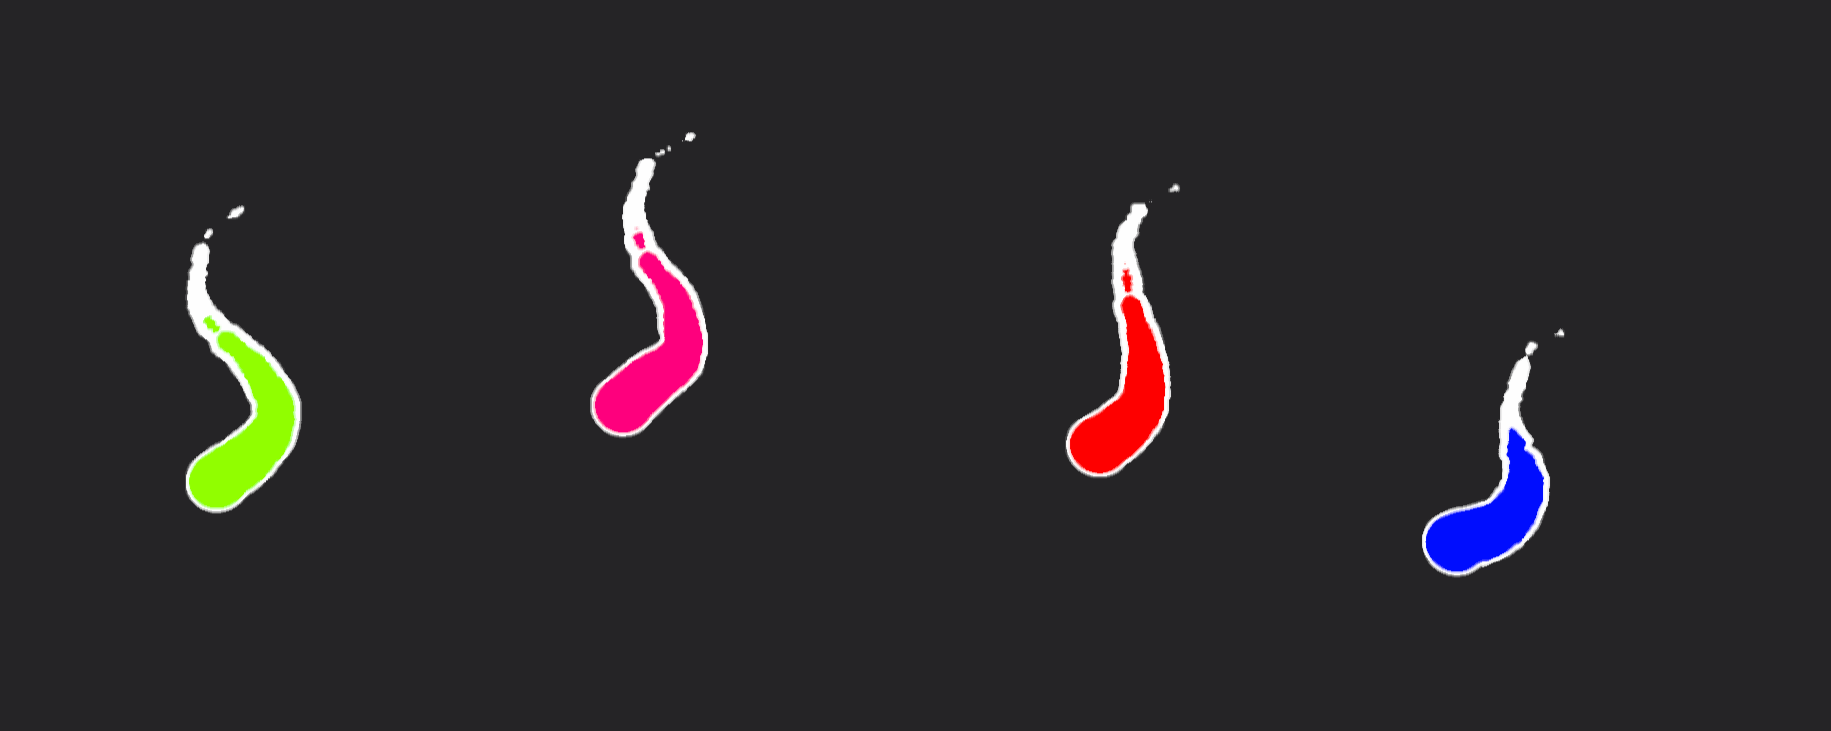
\includegraphics[width=1\textwidth]{figures/touch_indicators.png}
            \captionof{figure}{Touch indicators for four fingers on the touch frame.}
            \label{fig:touch_indicators}
        \end{figure}

        This is implemented using a compute shader and a shader built with Unity's Shader Graph. A compute shader is a program that runs on the GPU outside of the normal rendering pipeline.\footnote{\url{https://docs.unity3d.com/Manual/class-ComputeShader.html}} It is most useful for executing highly parallel algorithms. In this case, the compute shader processes finger positions, performs calculations, and stores results in render textures. The Shader Graph shader then uses these textures to render finger trail indicators in every frame.

        Each render texture stores data for two fingers using two channels per finger per pixel. This results in five textures, each with dimensions matching the greatest nearest power of two between the screen width and height. One channel stores the reverse distance from the pixel to the center of the finger trail, ranging from 1 (closest to the center) to 0 (outside the trail radius), similar to a signed distance function. The other channel records the decay of the pixel, where 1 indicates the most recent position, and 0 indicates total decay. These channels are depicted in Figure \ref{fig:touch_progress}, with red representing the distance to the trail's center and blue representing the decay.
        
        \begin{figure}[h!]
            \centering
            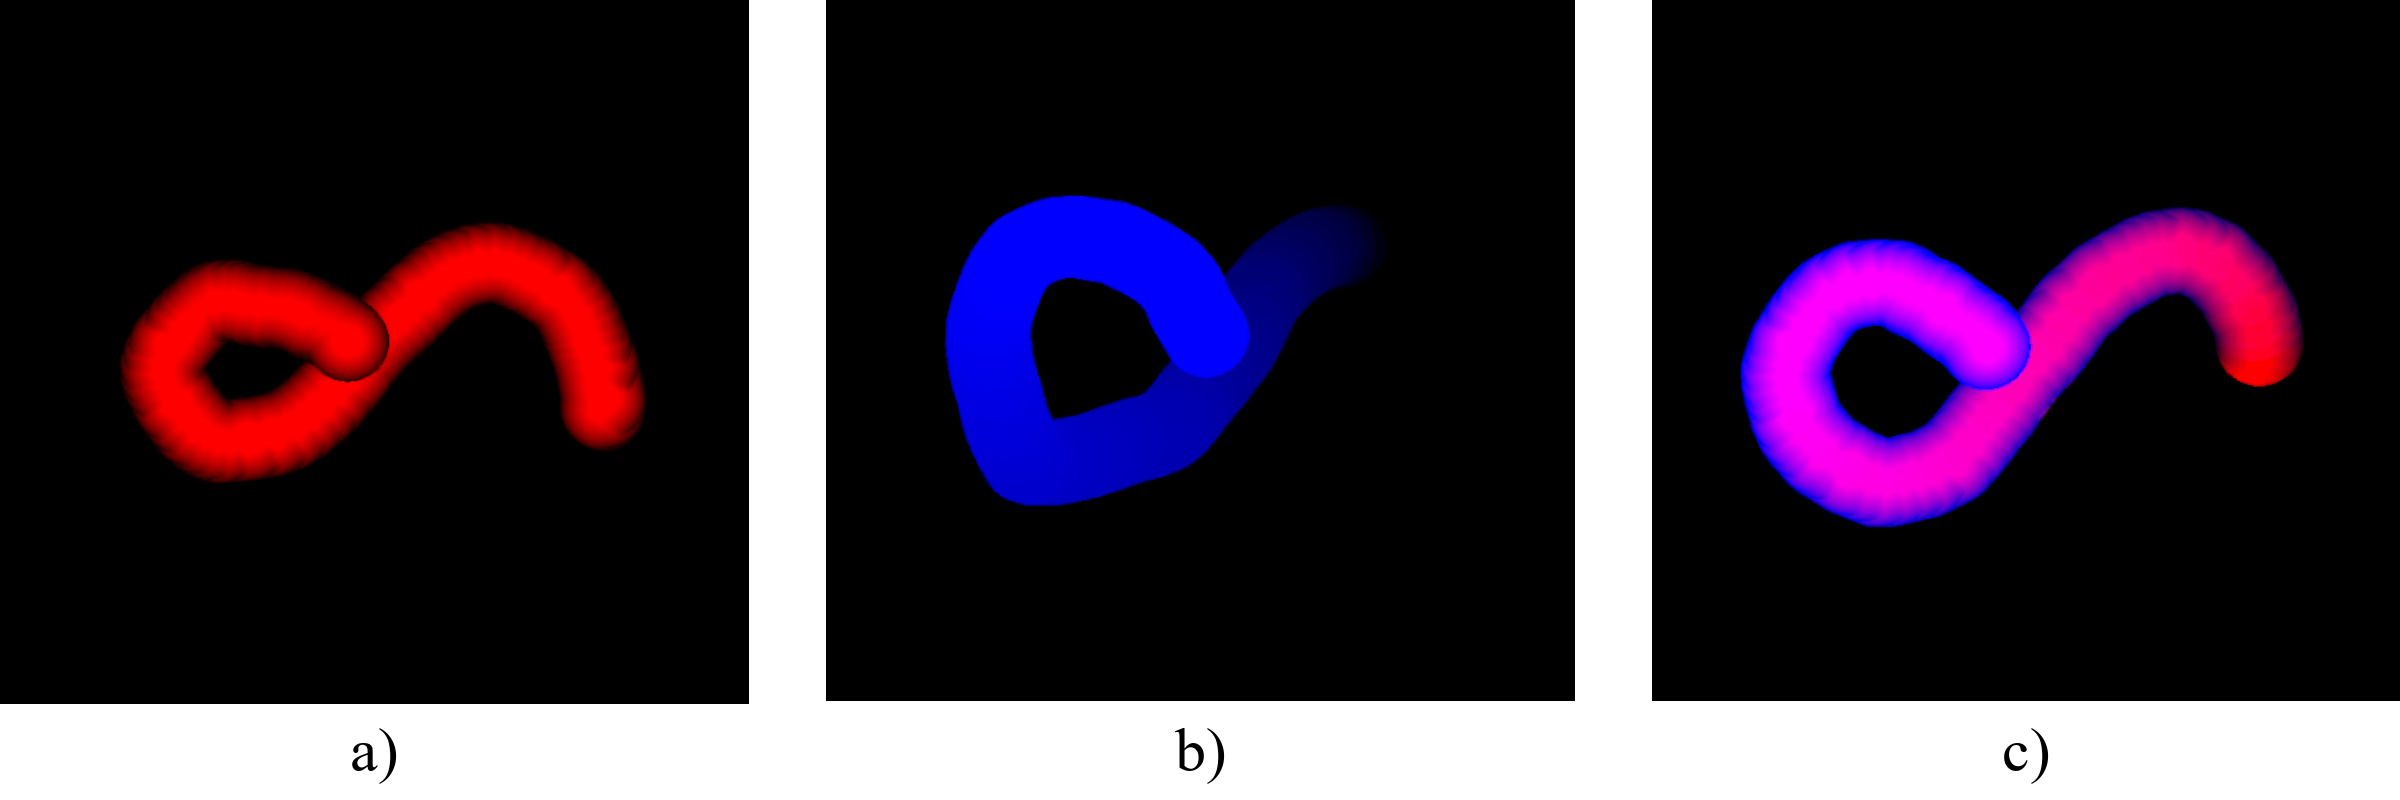
\includegraphics[width=1\textwidth]{figures/touch_progress.png}
            \captionof{figure}{The different components stored on the render texture for each finger: a) reverse distance to center; b) decay; c) distance and decay combined.}
            \label{fig:touch_progress}
        \end{figure}

        A compute shader function is executed by several compute shader thread groups for each of the three dimensions: \(X\), \(Y\), and \(Z\). In this case, the function defines for each group 8 threads for the \(X\) dimension, representing the pixel coordinate on the X axis, 8 threads for the \(Y\) dimension, representing the pixel coordinate on the Y axis, and 1 thread for the \(Z\) dimension, representing the render texture being processed. When the compute shader is executed, it runs using \(\text{texture}_{\text{width}} / 8\) groups on the \(X\) axis, \(\text{texture}_{\text{height}} / 8\) groups on the \(Y\) axis, and 5 groups on the \(Z\) axis, one for each render texture.

        The compute shader takes several inputs: five different render textures, two \lstinline{float4} structured buffers of size 5 (one for the current finger positions and one for the finger positions of the previous frame), a \lstinline{float} structured buffer of size 10 that stores the average inclination of each finger trail, a linear decay rate $\delta$, a finger radius in pixels $r$, and the time elapsed between the last frame and the current frame in seconds $\Delta t$. Each \lstinline{float4} vector in the structured buffers represents the screen-space coordinates of two fingers, with the first two floats for one finger and the next two floats for another finger.

        A simplified description of the algorithm for each finger and each pixel operates as follows: first, it calculates the decay \(\lambda_i\) of the pixel using the previous frame's decay value \(\lambda_{i-1}\) by computing \(\lambda_{i-1} - \delta \cdot \Delta t\). Next, it calculates the distance \(d\) and reverse distance $d_{\mathrm{rev}}$ from the pixel to the line segment that starts at the finger's position in the previous frame and ends at the current finger position. This calculation, shown in Equation \ref{eq:distance_line}, creates a capsule-like shape. In this equation, \(A\) is the finger's position in the last frame, \(B\) is the current finger's position, \(r\) is the line's thickness, and \(P\) is the pixel's position.

        \begin{figure}[h]
        \begin{equation}
        \begin{split} \label{eq:distance_line}
            \vec{AB} &= B - A \\
            \vec{AP} &= P - A \\
            h &= \mathrm{clamp} \left( \frac{\vec{AP} \cdot \vec{AB}}{\vec{AB} \cdot \vec{AB}} , 0, 1\right)  \\
            d &= \frac{\| \vec{AP} - h \cdot \vec{AB} \|}{r} \\
            d_{\mathrm{rev}} &= \mathrm{clamp} \left( 1 - d , 0 , 1\right)
        \end{split}
        \end{equation}
        \end{figure}

        %Then, it calculates how much the pixel is in front of the line segment using the calculating $h$ described in Equation \ref{eq:distance_line}, where $B$ is instead $(A_x + r \cdot \cos{\bar{m}}, A_y + r \cdot \sin{\bar{m}})$, where $\bar{m}$ is the average incline of the finger trail. The average incline is used instead of $B$ because often the line segments between frames are very small and one directional due to high refresh rates, resulting in visual artifacts.

        %Next, it checks whether the previously stored distance is still valid by checking whether $\lambda_i$ is less than $$~


        Based on how much the pixel is in front of the line segment, considering the average inclination of the finger trail, the algorithm linearly interpolates between \(\max\left(d_{\text{rev}}, d_{\text{rev}_{i-1}}\right)\) and \(d_{\text{rev}}\) to calculate the value to store in the render texture. This approach allows the finger trail to overlap at the front and smoothly blend behind. The final decay value stored in the texture is \(\lambda_i\), with an additional 1 added if \(d \leq 1\), clamped between 0 and 1.

        Finally, the fragment shader samples each render texture. It subtracts the decay value from the distance to create a shrinking effect, applies a border by comparing the resulting value with a threshold, and assigns a color based on the finger's order.

        \begin{figure}[h!]
            \centering
            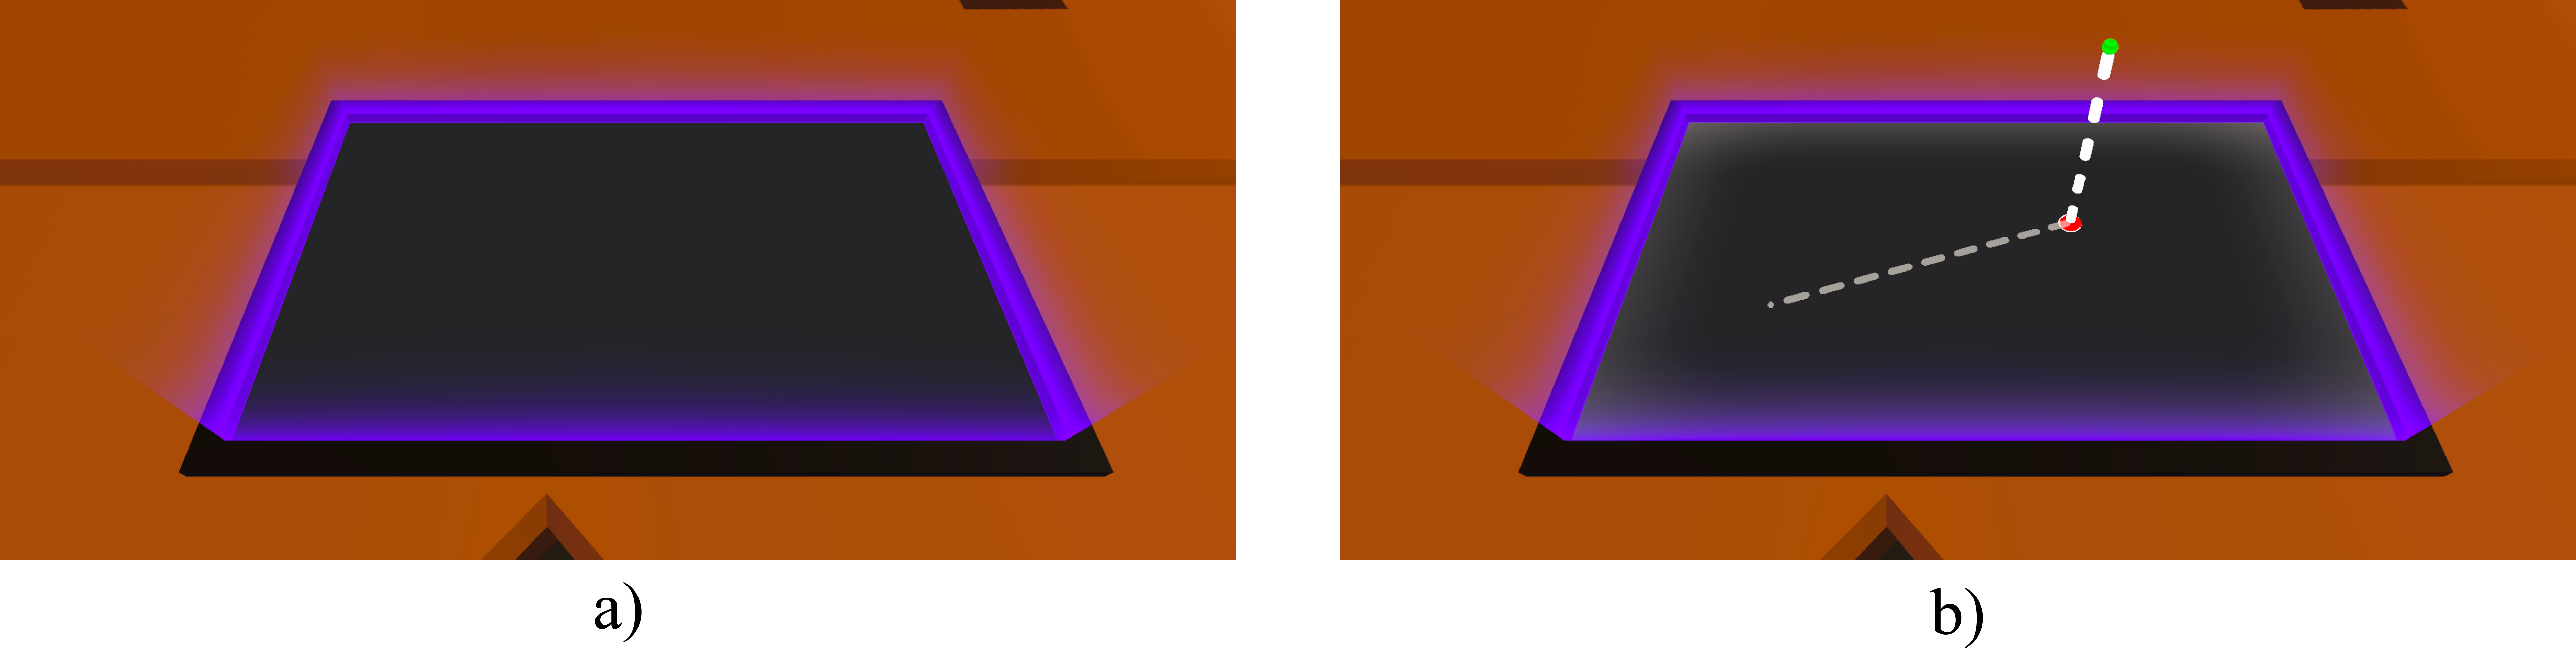
\includegraphics[width=1\textwidth]{figures/frame_glow.png}
            \captionof{figure}{Glow effect indicating gesture detection on the touch surface. (a) The initial state with no gesture detected. (b) The glow effect activates when a gesture is detected.}
            \label{fig:frame_glow}
        \end{figure}

        The virtual touch frame illuminates with a glowing effect whenever the system detects vertical transform or balloon selection gestures, signaling the user that their gesture has been recognized. This glow effect, demonstrated in Figure \ref{fig:frame_glow}, is achieved using a shader that uses a rounded box signed distance function.\footnote{\url{https://www.shadertoy.com/view/Nlc3zf}} The strength of the glow is animated using the function $-\left(2 \sqrt{t} - 1\right)^2 + 1$, where \(t\) represents the elapsed time since the animation began. Initially, this function rises quickly until the result reaches 1 at $t = 0.25$, after which it gradually diminishes. The animation halts at \(t = 0.8\) and resumes from that point when the gesture concludes.
                    


        %\begin{figure}[h!]
        %    \centering
        %    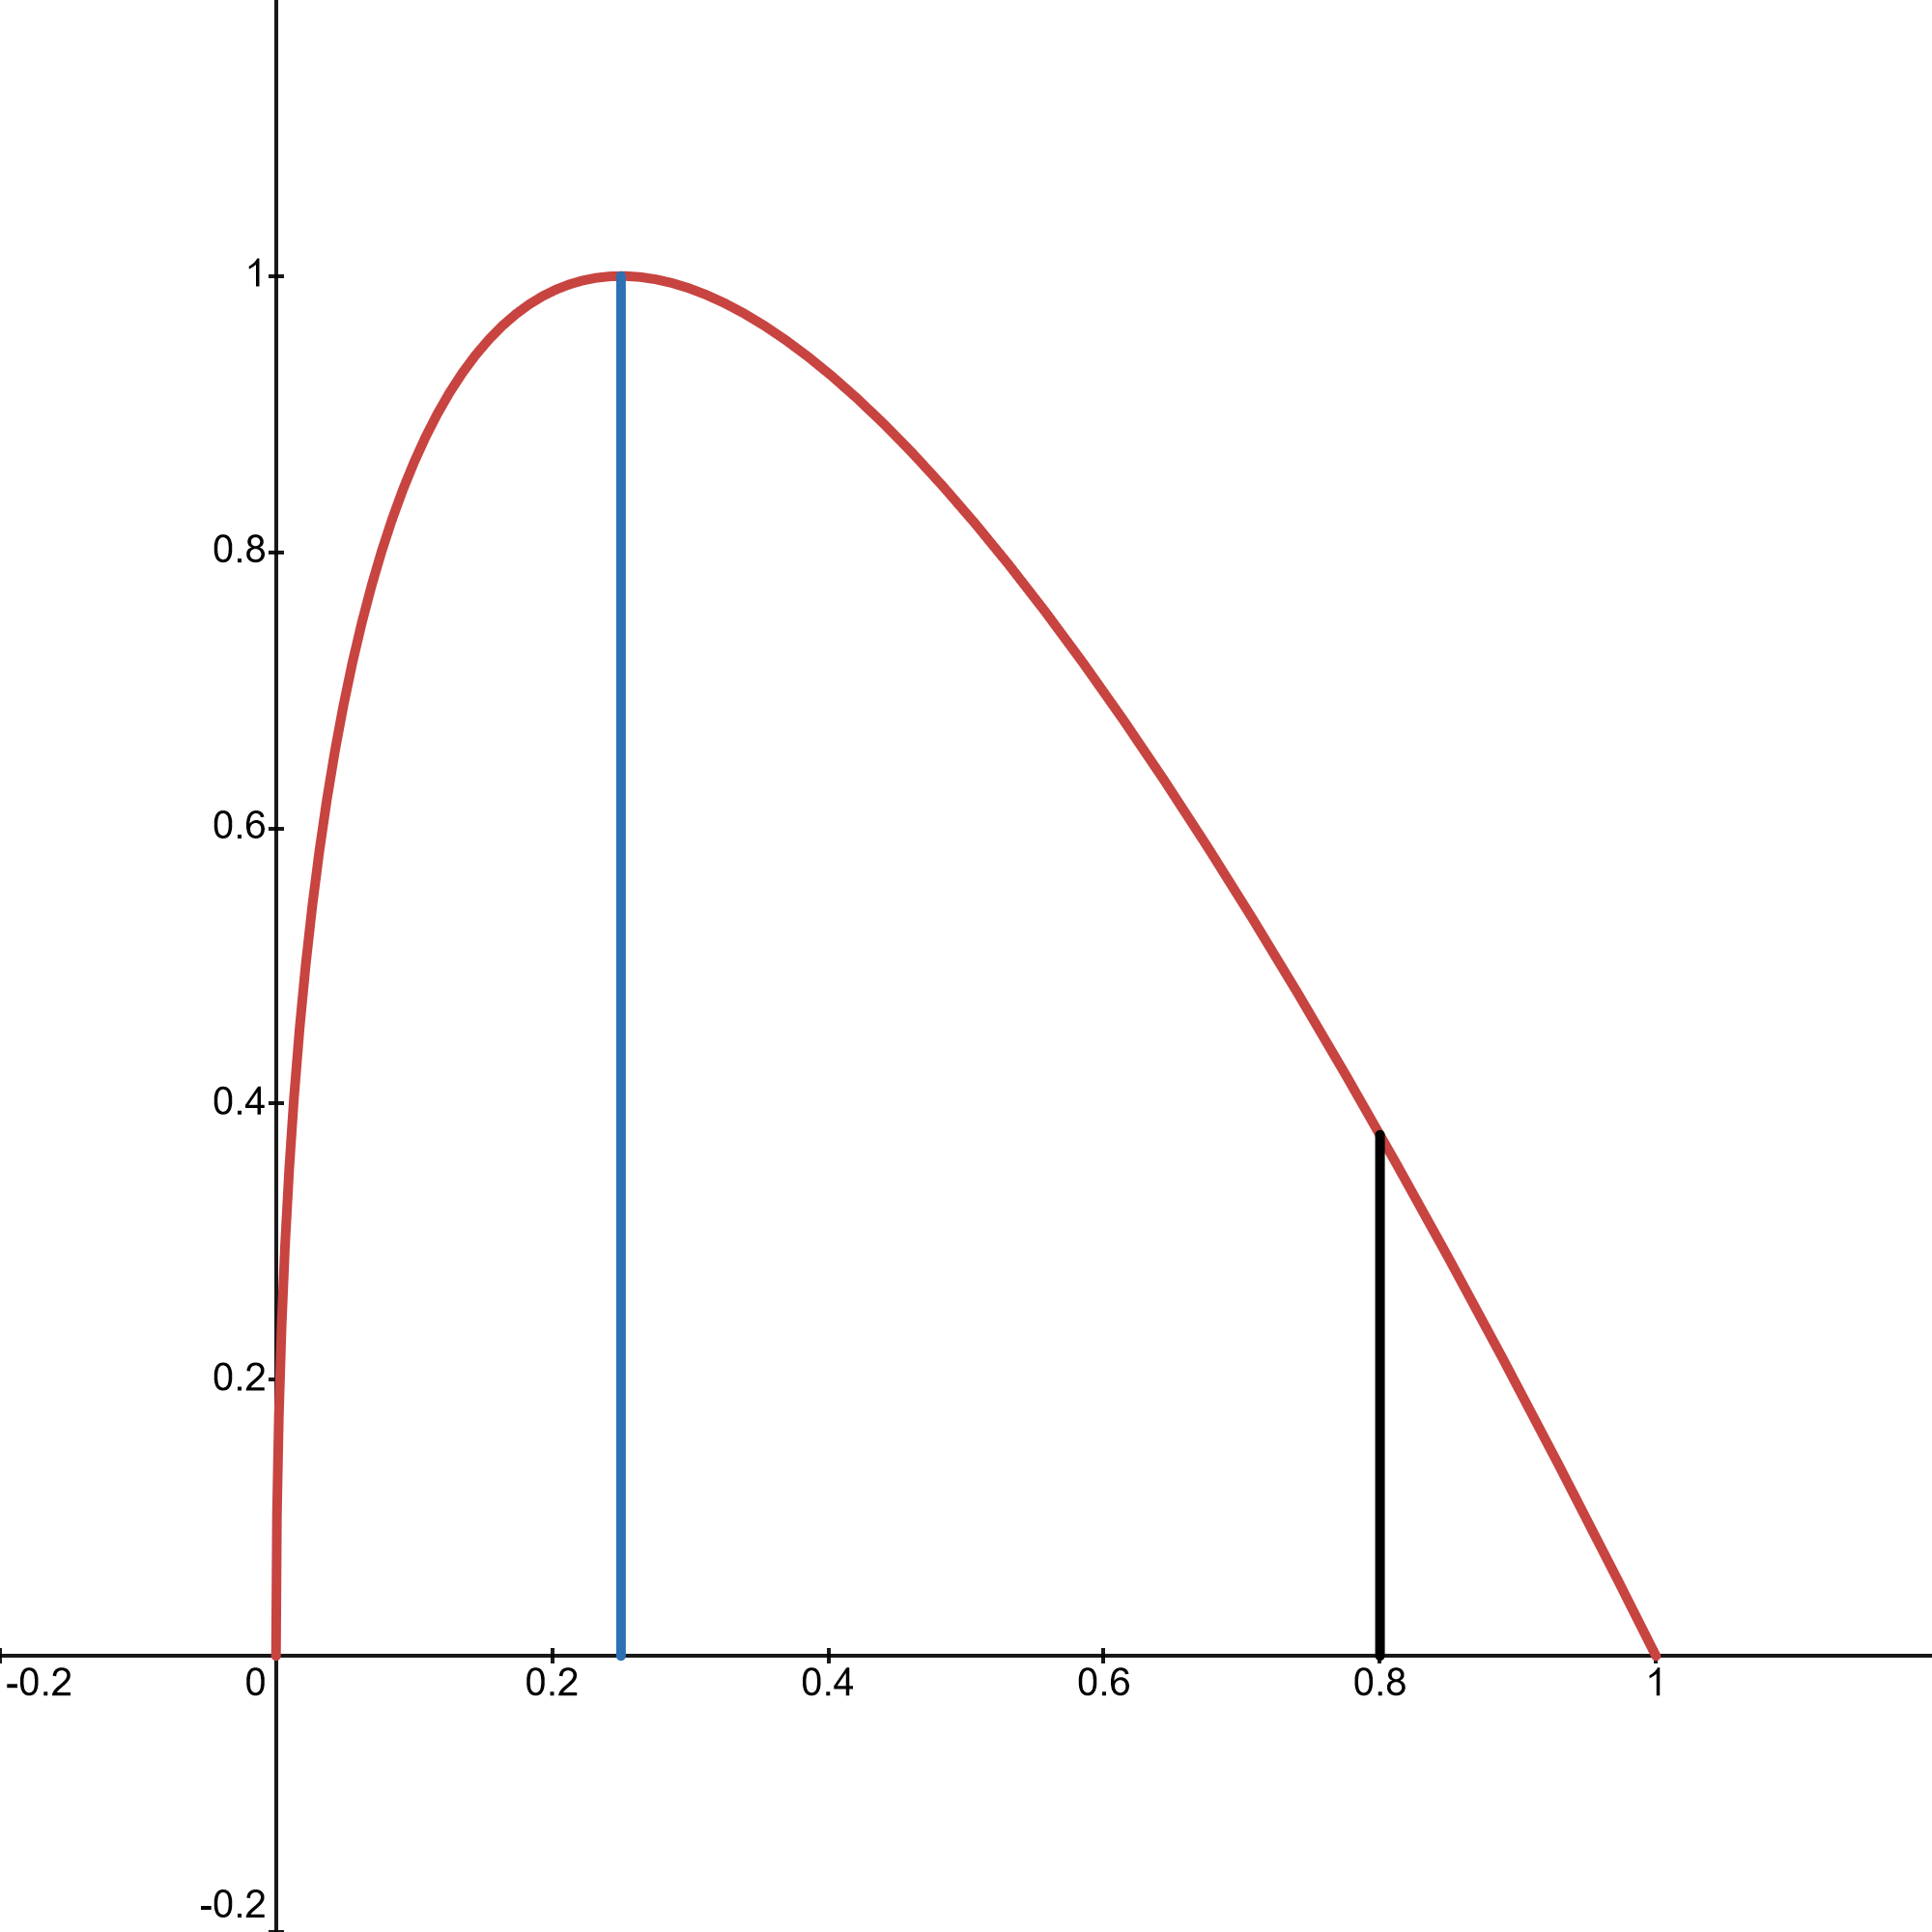
\includegraphics[width=0.5\textwidth]{figures/frame_glow_f.png}
        %    \captionof{figure}{Animation curve for the strength of the glow effect. The blue line at \( t = 0.25 \) indicates the point of maximum strength, and the line at \( t = 0.8 \) marks where the animation halts.}
        %    \label{fig:frame_glow}
        %\end{figure}
    
    
    \subsection{Frame Limit Indicator} \label{sec:frame_limits}

        The balloon's position on the XZ axis during balloon selection is constrained by the boundaries of the virtual touch frame. To help users understand these boundaries, even when the frame is obscured by the replica, a purple illumination effect outlines the limits. This effect is shown in Figure \ref{fig:frame_limits}.

        \begin{figure}[h!]
            \centering
            \includegraphics[width=1\textwidth]{figures/frame_limits.png}
            \captionof{figure}{Illumination effect on the replica indicating the limits of the touch frame.}
            \label{fig:frame_limits}
        \end{figure}
    
        The illumination effect is achieved using a shader applied to a transparent rectangular prism extending from the touch frame's base. The shader's primary function is to gradually diminish the illumination effect as the distance from the prism increases. This is accomplished using a modified version of a shader initially designed for a stylized water effect\footnote{\url{https://ameye.dev/notes/stylized-water-shader/}}, created using Unity's Shader Graph.
        
        To calculate the distance \( d \), a vector \(\vec{CA}\) is obtained from the camera to the fragment's position on the prism using the View Vector node. This vector is then normalized to \(\hat{v}\). The depth texture is sampled to obtain the distance from the camera to the point occluded by the prism, \(|CB|\). The normalized vector is multiplied by this distance, resulting in \(\vec{CB} = \hat{v} \cdot |CB|\). Adding this vector to the camera's position gives the position of the occluded point, \( B = C + \vec{CB} \). The distance vector \(\vec{BA}\) is obtained by subtracting the occluded point's position from the fragment's position on the prism's surface, \(\vec{BA} = A - B\). Finally, the length of this vector is calculated to obtain the distance, \( d = \|\vec{BA}\| \).
        
        \begin{figure}[h!]
            \centering
            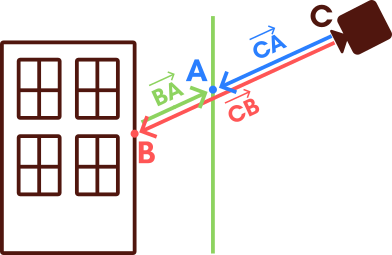
\includegraphics[width=.5\textwidth]{figures/limit_calc.png}
            \captionof{figure}{Diagram illustrating the steps to calculate $d$.}
            \label{fig:limit_calc}
        \end{figure}
    
        To achieve the gradual effect, the function \( x = e^{-\frac{d}{0.05}} \) is applied. This ensures that when \( d = 0 \), the effect is at full power, declines rapidly, and then tapers off. This behavior is shown in graph a) of Figure \ref{fig:limit_func}. To soften the effect at the borders, the function described in Equation \ref{eq:limit_calc} and depicted in graph b) of Figure \ref{fig:limit_func} is applied to \( x \). This adjustment causes the effect to start at 0.2 power at the border, rise smoothly to 0.8 power, and then taper off as the distance increases. This progression is illustrated in graph c) of Figure \ref{fig:limit_func}.

        The function \( -37.5 x^3 + 82.5 x^2 - 60 x + 15.2 \) was derived from a cubic polynomial for creating a smooth curve between two points: \((c, m)\) and \((k, m + b)\), shown in Equation \ref{eq:limit_poly}.\footnote{\url{https://math.stackexchange.com/a/2209953}} In this case, the parameters are \( c = 0.8 \), \( m = 0.8 \), \( k = 1 \), \( b = -0.6 \), \( p = 0 \), and \( q = -1.5 \).

        \begin{figure}[h]
        \begin{equation} \label{eq:limit_calc}
        \alpha =
        \begin{cases}
            x & \text{if} \quad x \leq 0.8 \\
            -37.5 x^3 + 82.5 x^2 - 60 x + 15.2 & \text{if} \quad x > 0.8 \\
            0.2 & \text{if} \quad x > 1
        \end{cases}
        \end{equation}
        \end{figure}

      \begin{figure}[h]
        \begin{equation} \label{eq:limit_poly}
        \left(p+q-2\cdot b\right)\cdot\left(\frac{x-c}{k-c}\right)^{3}\ +\ \left(3\cdot b\ -\ 2\cdot p-q\right)\cdot\left(\frac{x-c}{k-c}\right)^{2\ }+\ p\ \cdot\ \left(\frac{x-c}{k-c}\right)+m
        \end{equation}
        \end{figure}

                
        \begin{figure}[h!]
            \centering
            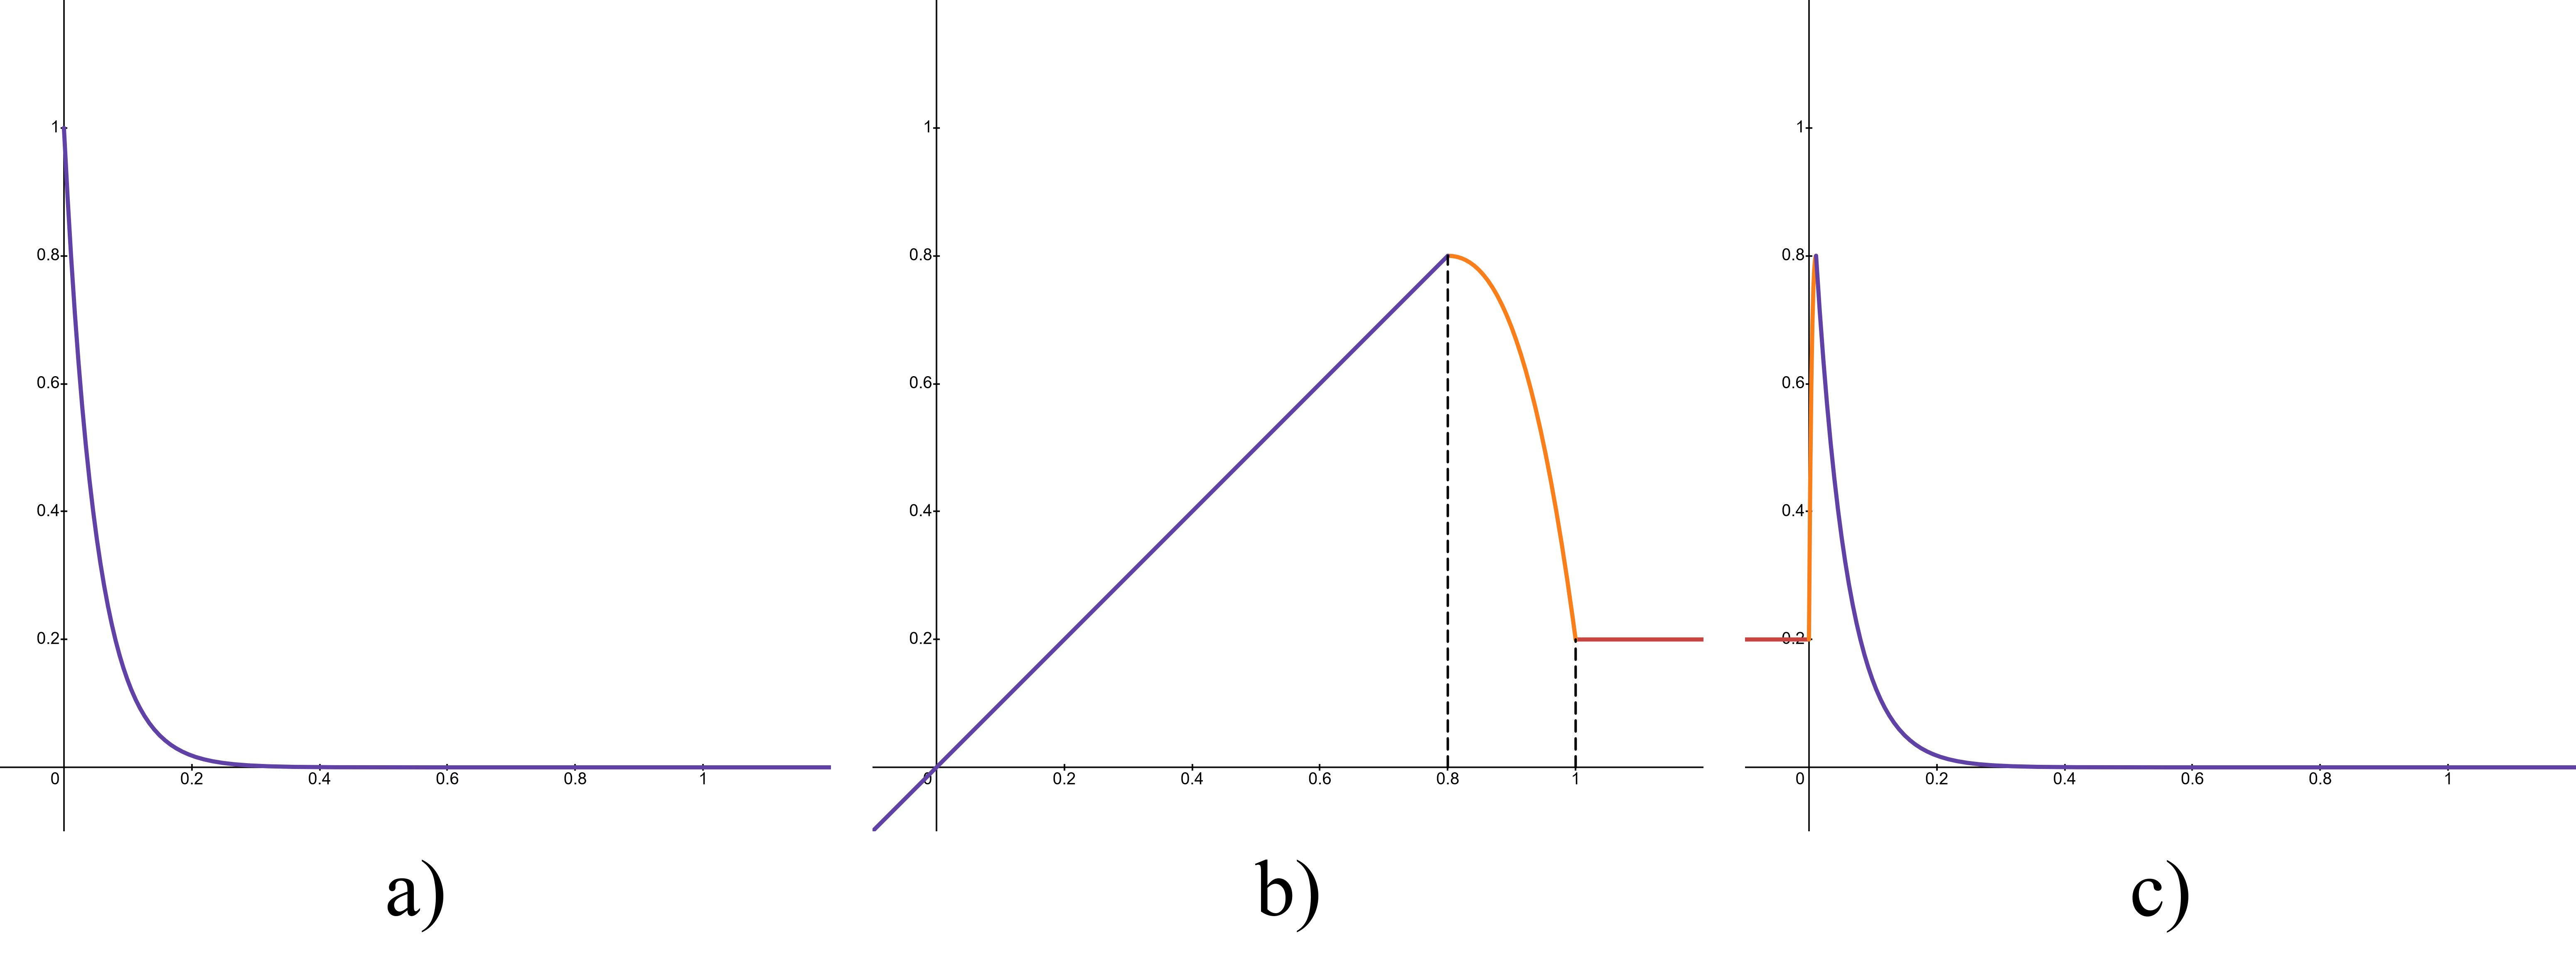
\includegraphics[width=1\textwidth]{figures/limit_func.png}
            \captionof{figure}{Graphs illustrating the functions used to modify the intensity of the limit illumination effect. Graph a) shows \( e^{-\frac{d}{0.05}} \) where the horizontal axis represents distance \( d \). Graph b) displays the function described in Equation \ref{eq:limit_calc}, with the horizontal axis representing \( x \). Graph c) depicts the function from Equation \ref{eq:limit_calc} with the horizontal axis representing distance \( d \). }
            \label{fig:limit_func}
        \end{figure}

    \subsection{Virtual Table} \label{sec:virtual_table}

        As shown in the literature \cite{zielaskoMenusDeskSystem2019, sousaVRRRRoomVirtualReality2017, zielaskoNonStationaryOfficeDesk2019}, the presence of a virtual table can be helpful in presenting information. This prototype uses the virtual touch frame described in Section \ref{sec:touch_frame} to represent that information. While the table is useful for displaying information, it can obscure much of the to-scale model, especially if the user wants to look down. To make it less intrusive, the table begins to fade and becomes invisible after 2 seconds of the touch surface not detecting any fingers, as shown in Figure \ref{fig:table_visibility}.

        \begin{figure}[h!]
            \centering
            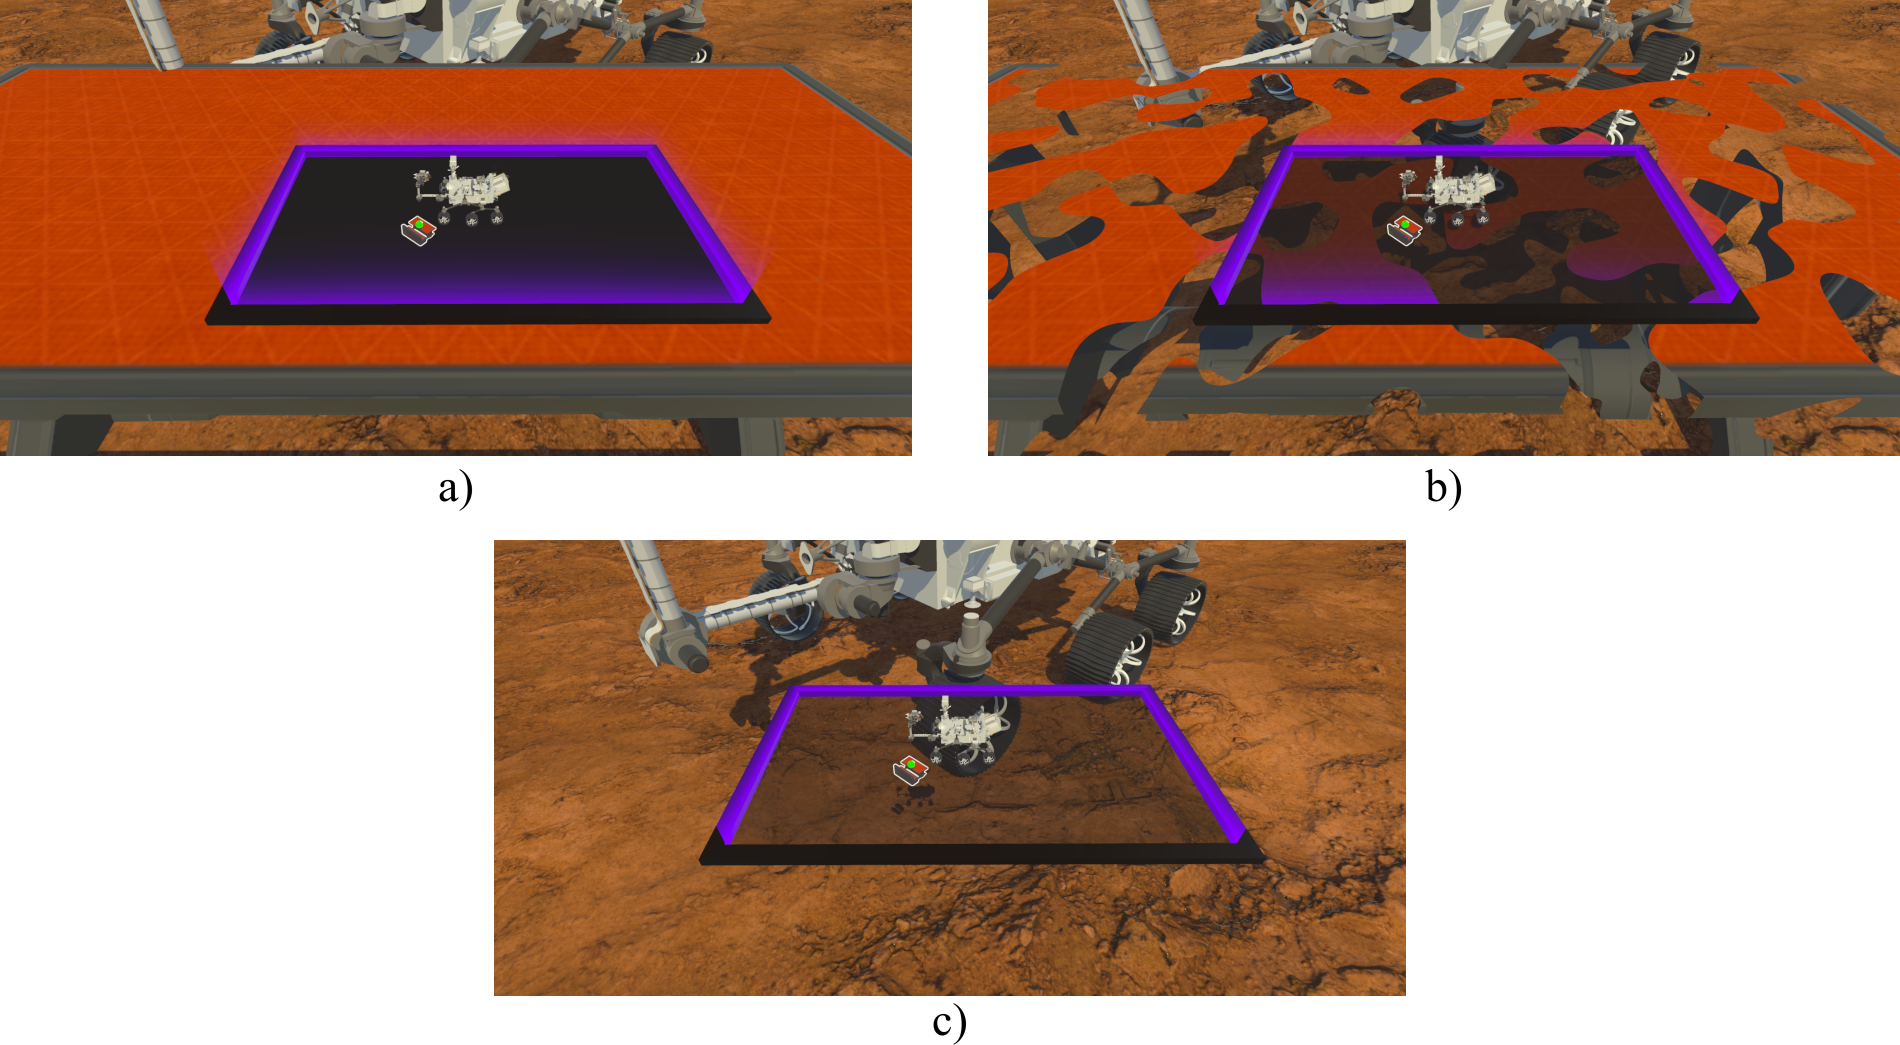
\includegraphics[width=1\textwidth]{figures/table_visibility.png}
            \captionof{figure}{The transition of the virtual table from: a) fully visible; b) half-visible; c) fully invisible.}
            \label{fig:table_visibility}
        \end{figure}

        This effect is achieved using a shader that takes the pixel's world space position and applies a simplex 3D noise function\footnote{\url{https://github.com/JimmyCushnie/Noisy-Nodes}} to determine the pixel's alpha clip threshold. After 2 seconds of inactivity, the table's alpha value is reduced using a smooth animation curve. The alpha clip threshold then determines whether a pixel is visible or invisible. Alpha blending was not used because it caused visual artifacts, making the table visible from behind itself.

        User tables are also visible in the replica as miniatures, as shown in Figure \ref{fig:table_behind} and described in Section \ref{sec:awareness}. These miniatures feature an outline effect to help them stand out from the surrounding environment, using a free Unity package.\footnote{\url{https://assetstore.unity.com/packages/tools/particles-effects/quick-outline-115488}} They also glow intermittently to draw attention, increasing the lightness of the table's color through an animation using a quadratic easing in-out function.\footnote{\url{https://assetstore.unity.com/packages/vfx/shaders/shader-graph-easing-193427}} The miniatures display who is at the table by showing a user seated at it, as seen in image c) of Figure \ref{fig:table_behind}. These miniatures do not scale with the replica, keeping their size constant, similar to markers on a map.

        They remain visible behind objects in the replica to help users quickly identify their and others' tables. This is achieved by rendering the table miniature in an additional render pass using the depth buffer to determine the appropriate material. If the table is behind an object, it appears slightly transparent and in a single color; otherwise, it uses the normal material.\footnote{\url{https://docs.unity3d.com/Packages/com.unity.render-pipelines.universal@10.4/manual/renderer-features/how-to-custom-effect-render-objects.html}}

        \begin{figure}[h!]
            \centering
            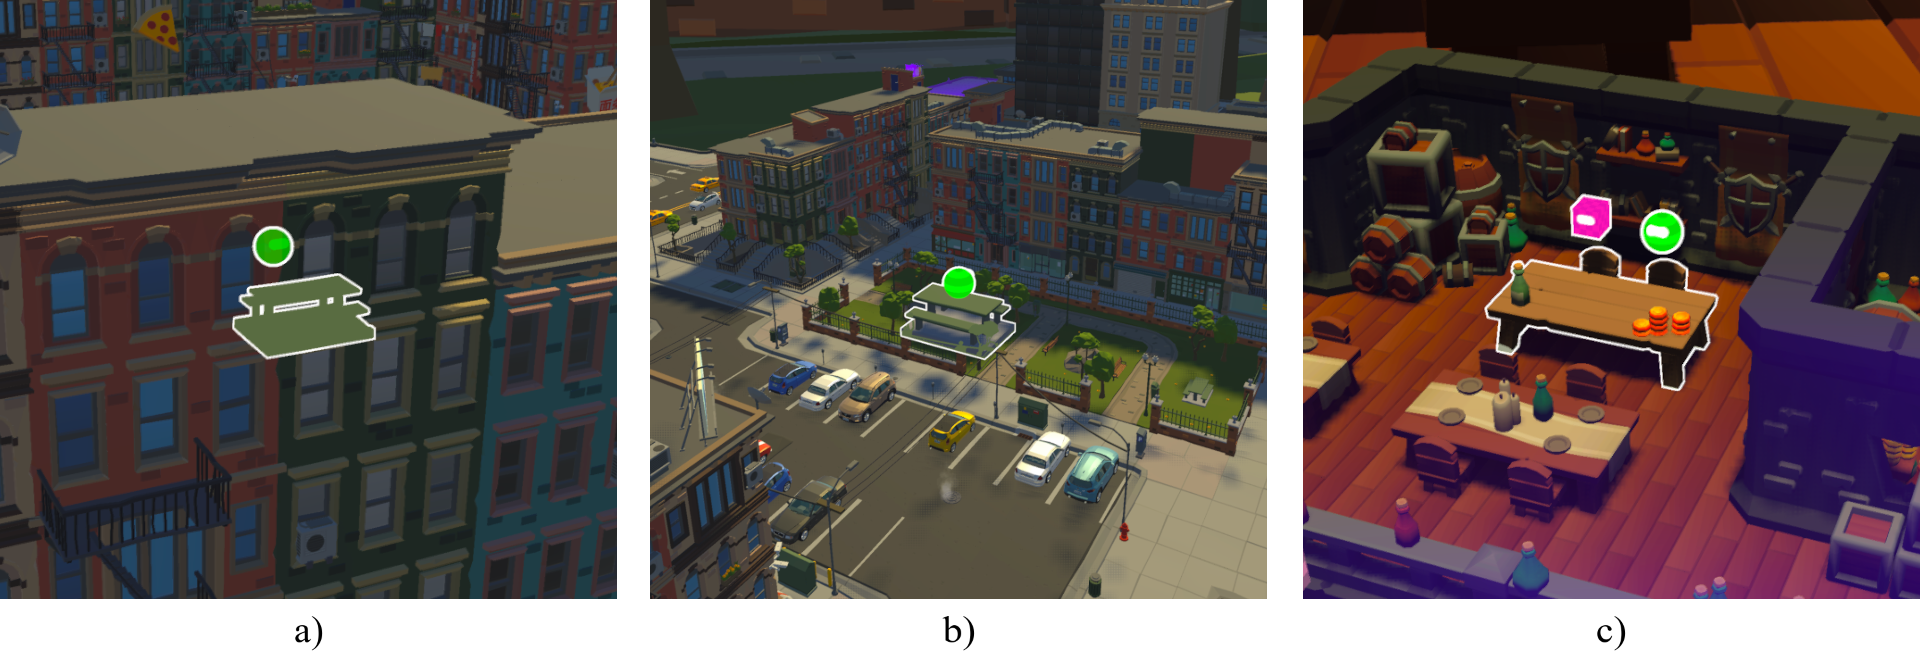
\includegraphics[width=1\textwidth]{figures/table_behind.png}
            \captionof{figure}{The table miniature visible in the replica. Image (a) shows the table behind an object, image (b) shows the table within the replica, and image (c) shows two users at the table.}
            \label{fig:table_behind}
        \end{figure}


    \subsection{Points of Interest} \label{sec:visual_poi}
        As mentioned in Section \ref{sec:awareness}, the points of interest reflect the appearance of their creators. Figure \ref{fig:poi_appearance} demonstrates this: the first user's points of interest are green-striped spheres, while the second user's are purple checkerboard cubes. Each point of interest is marked with a number that rotates to face the camera and glows intermittently to draw attention, achieved using a Fresnel effect with a sine curve animation.

        \begin{figure}[h!]
            \centering
            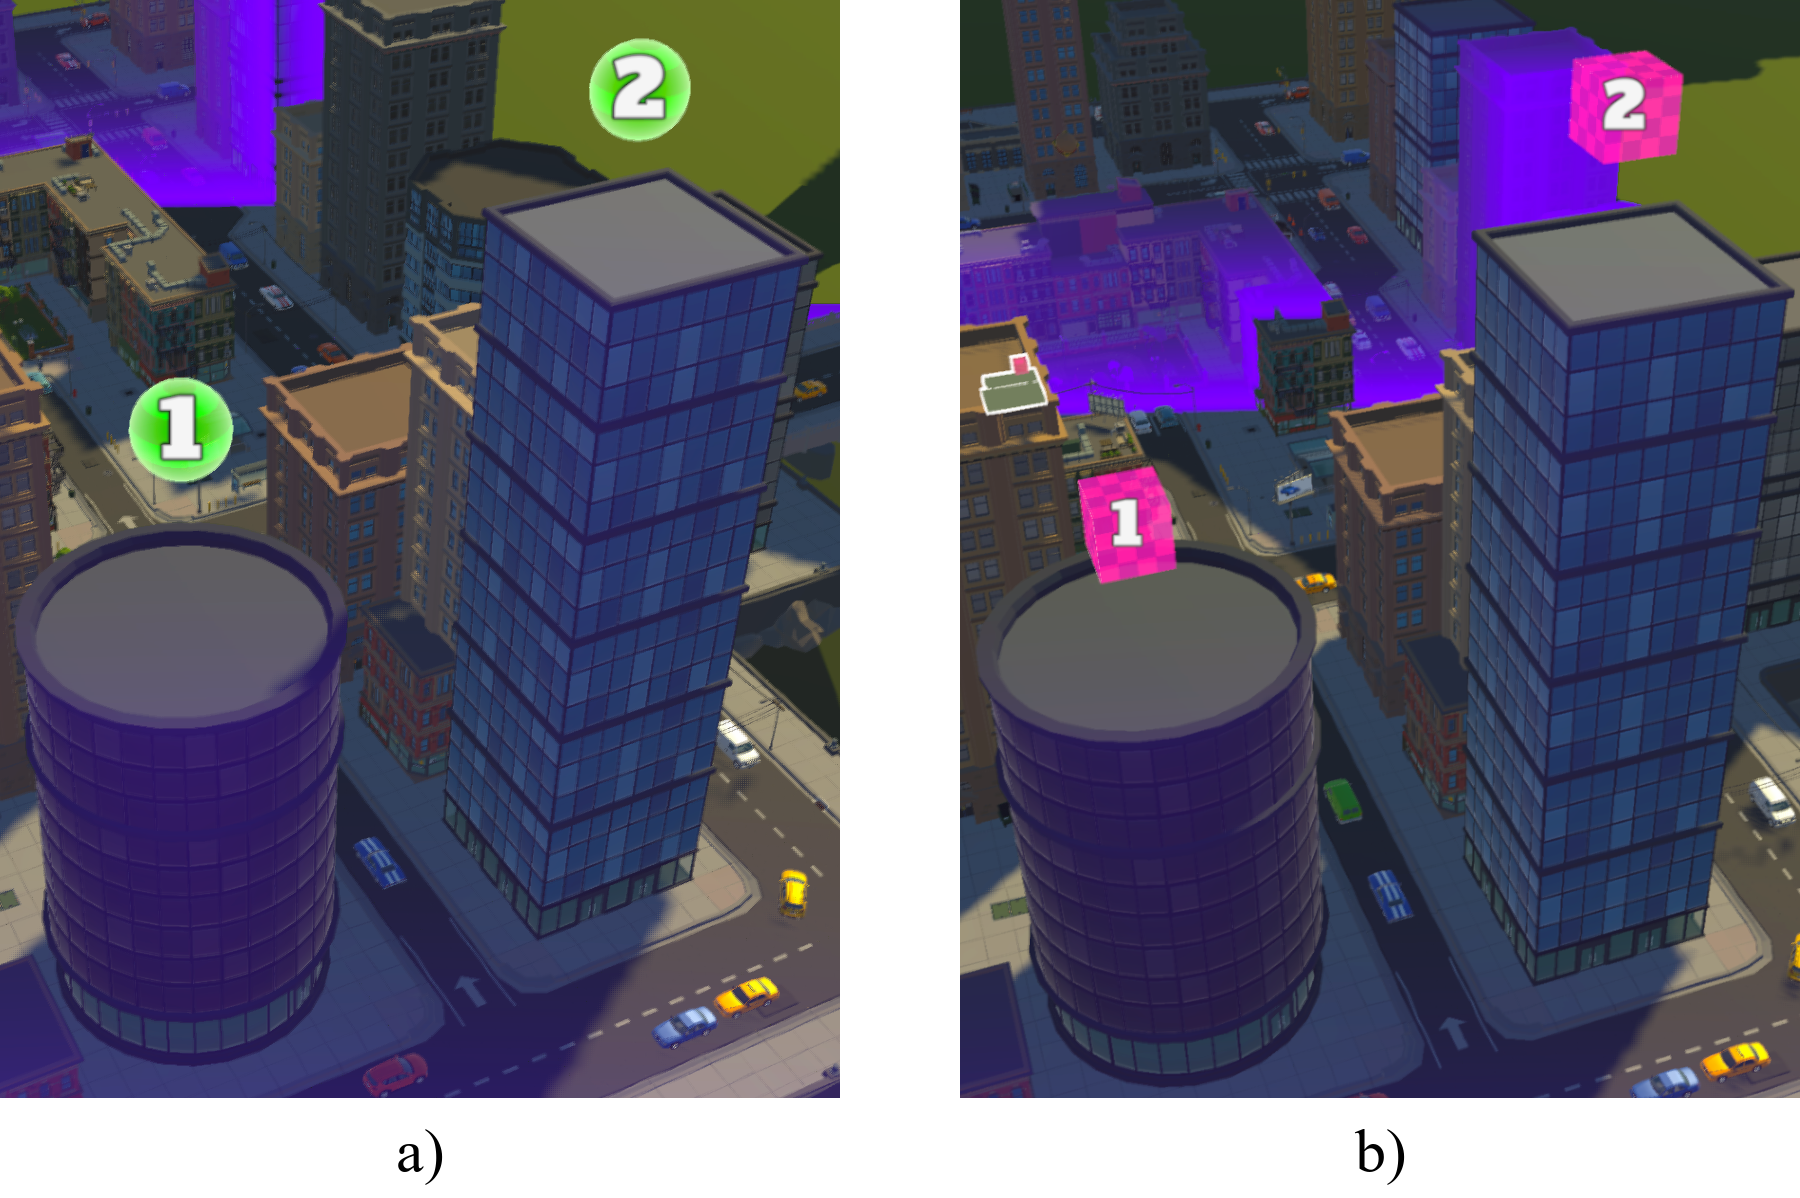
\includegraphics[width=.8\textwidth]{figures/poi_appearance.png}
            \captionof{figure}{Point of interest appearance based on the creator's appearance. Image (a) shows points of interest from the first user, and image (b) shows points of interest from the second user.}
            \label{fig:poi_appearance}
        \end{figure}

        Similar to the miniature tables, points of interest are visible behind objects in the replica and do not scale with the replica. This is shown in image (a) of Figure \ref{fig:poi_visibility}, where a point of interest is visible behind a building in the replica with a muted color and slight transparency. However, in the 3D model, the point of interest is not visible behind the building, as shown in image (b). This ensures that the points of interest do not distract or confuse users when looking at the replica. Points of interest in the 3D model scale with distance so users can see them from afar but do not become too large when close, preserving essential details.

       \begin{figure}[h!]
            \centering
            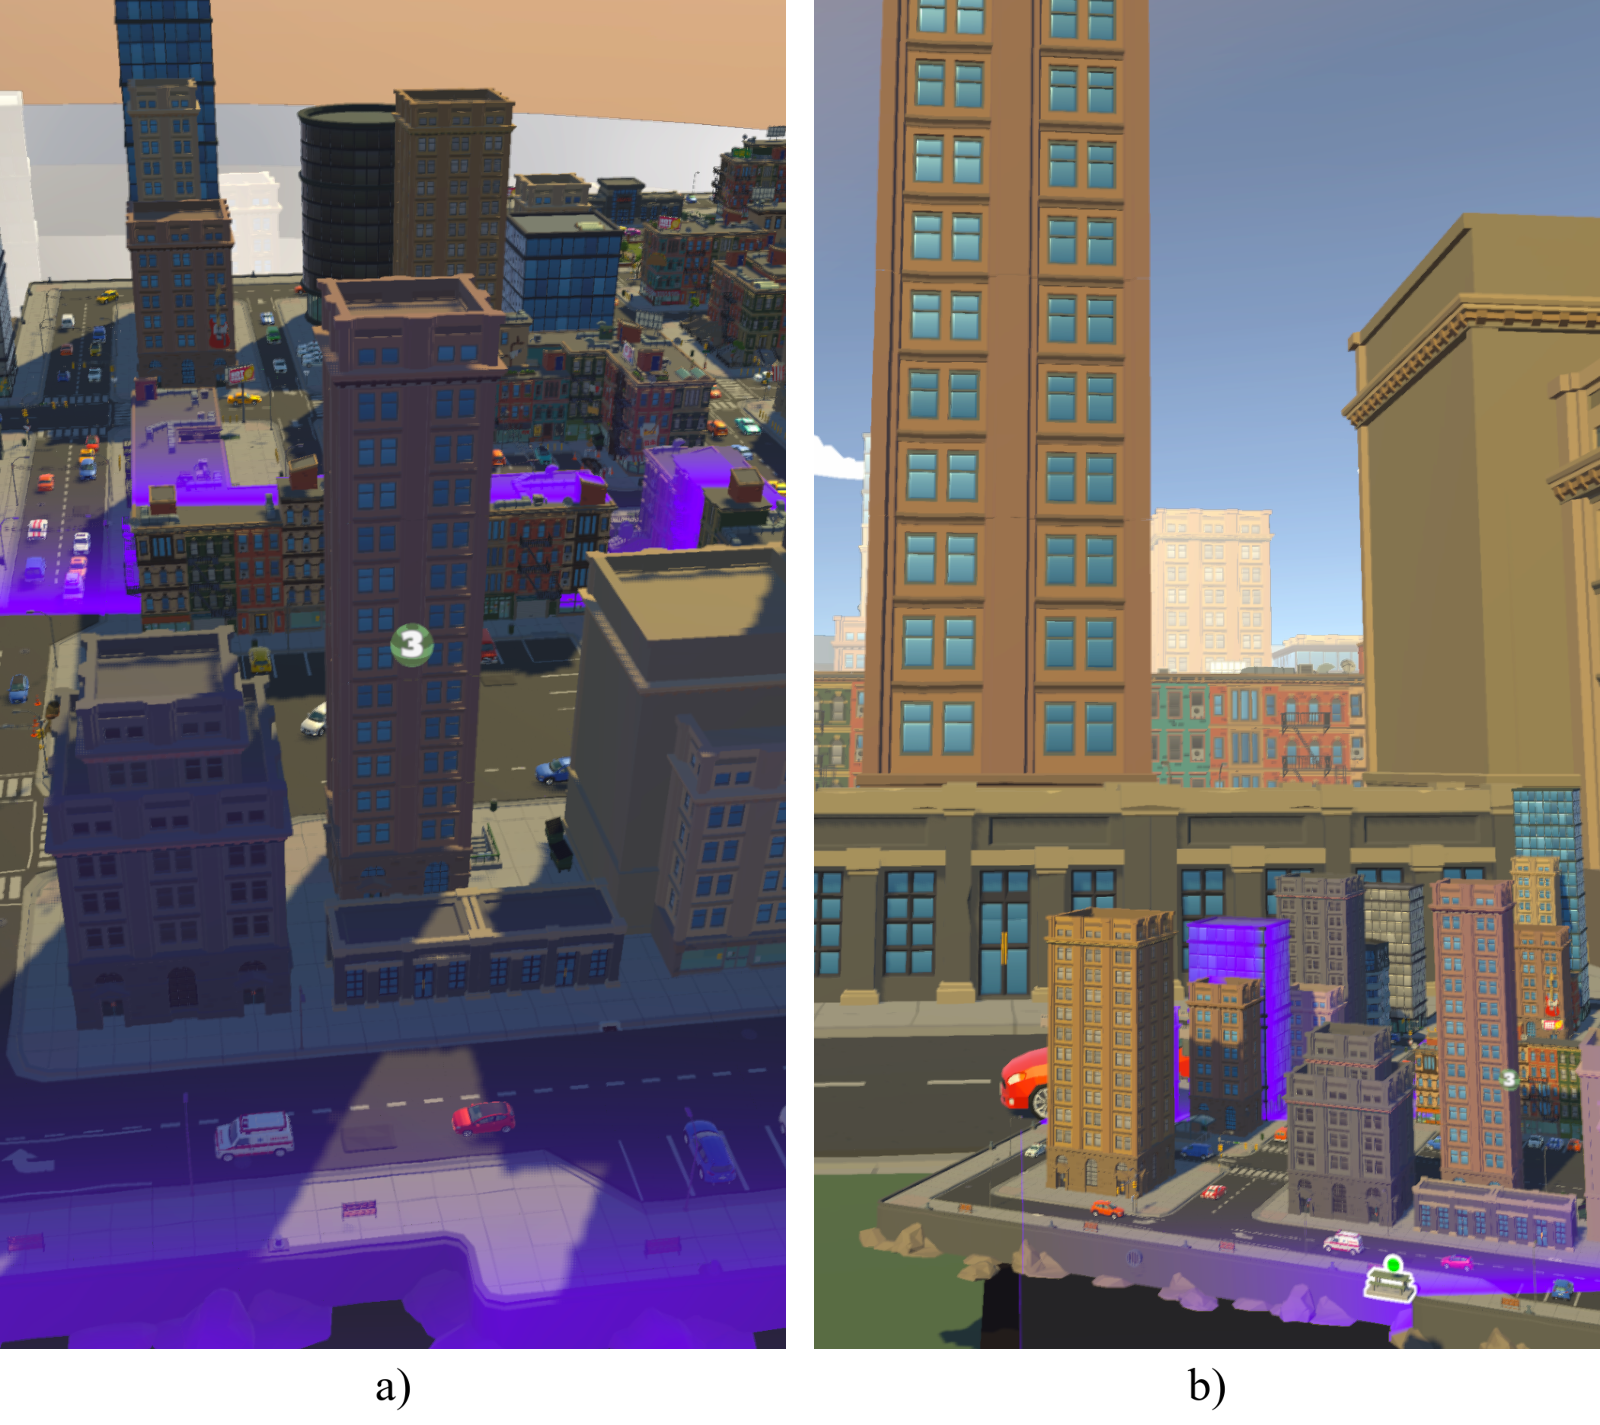
\includegraphics[width=.8\textwidth]{figures/poi_visibility.png}
            \captionof{figure}{Points of interest visibility. Image (a) shows a point of interest in the replica that is visible behind the building. Image (b) shows that the same point of interest is not visible in the 3D model behind the building.}
            \label{fig:poi_visibility}
        \end{figure}

        Points of interest created by another user that are not yet acknowledged are marked with a vertical line, as shown in Figure \ref{fig:poi_marker}. This line is capped with a symbol displaying the point of interest's identification number, resembling the point of interest's appearance to help users quickly identify unacknowledged points. The line and symbol always face the user using a vertical billboard effect. The line is also visible behind objects in the replica and scales with distance, as seen in image (c) of Figure \ref{fig:poi_marker}, ensuring it can be seen from any angle. If the marker does not fit within the user's field of view, it flips upside down to remain visible, as shown in image (d) of Figure \ref{fig:poi_marker}.

       \begin{figure}[h!]
            \centering
            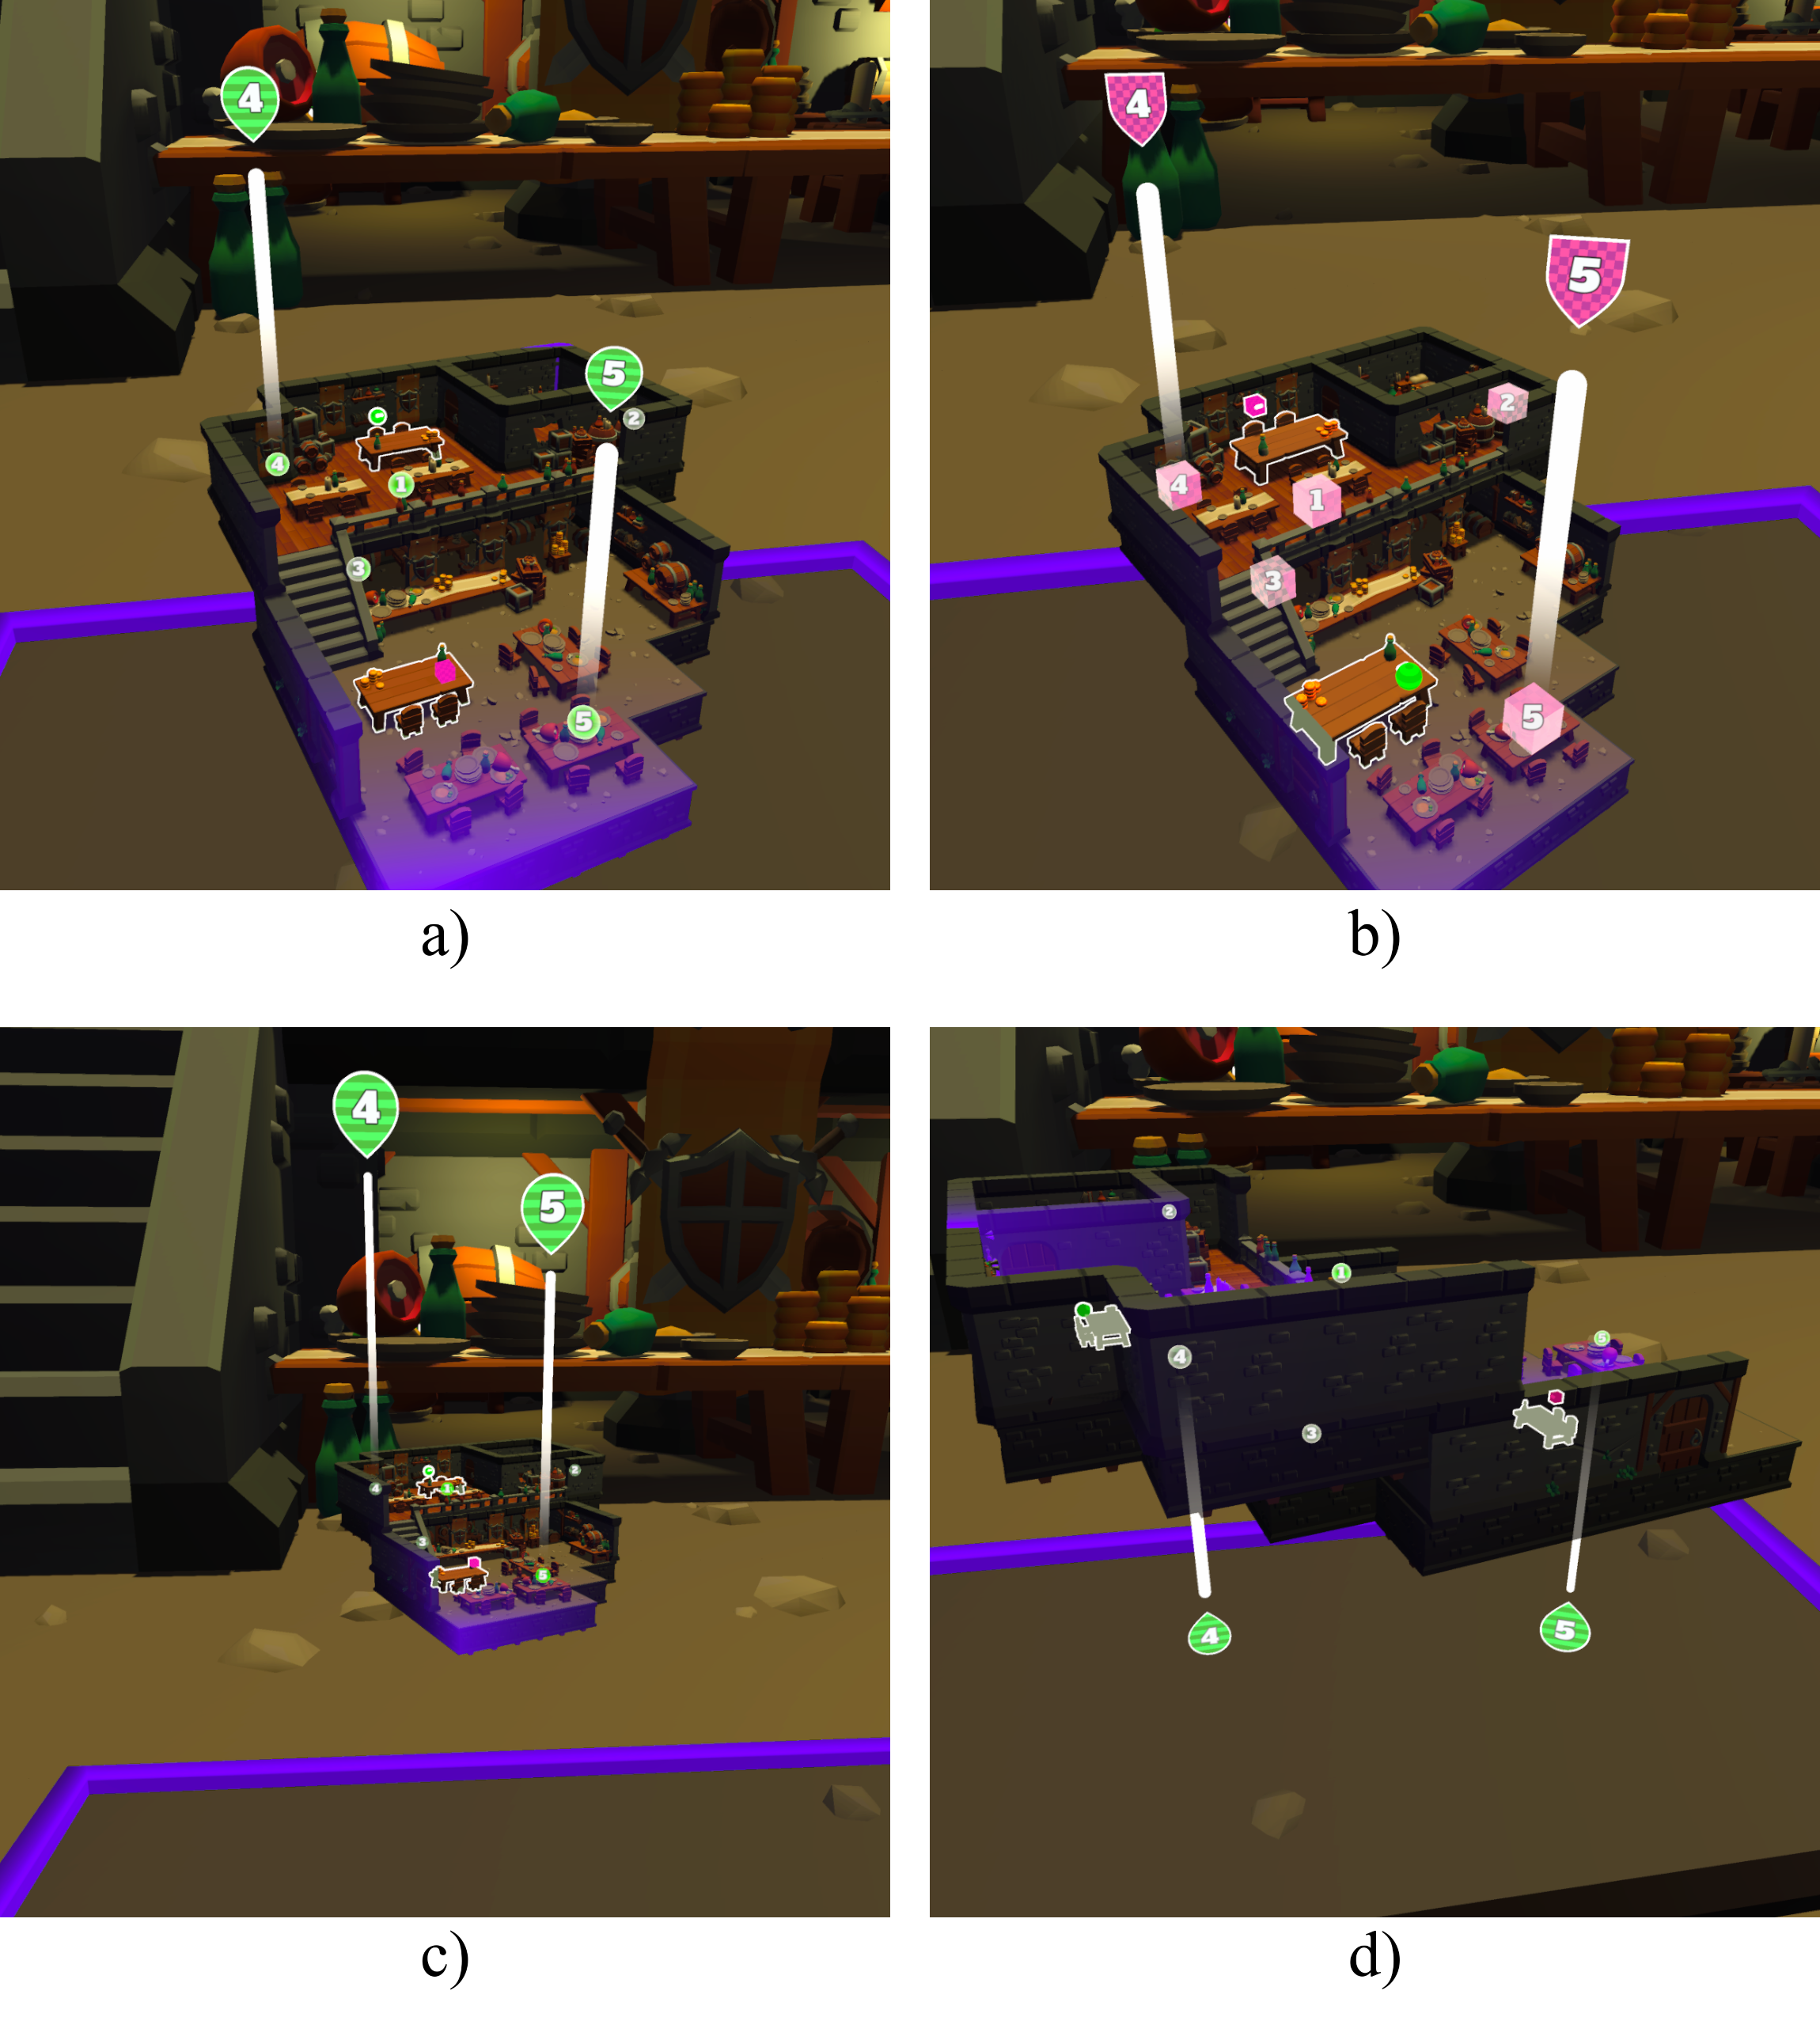
\includegraphics[width=1\textwidth, height=1\textheight, keepaspectratio]{figures/poi_marker.png}
            \captionof{figure}{Point of interest markers. Image (a) shows markers for the first user, and image (b) shows markers for the second user. Image (c) demonstrates the scaling of the markers with distance. Image (d) displays the markers flipped upside down to ensure they are always visible.}
            \label{fig:poi_marker}
        \end{figure}
        
    \subsection{Balloon Selection} \label{sec:visual_balloon}
        The balloon selection gesture is indicated by a set of dashed helper lines: one on the touch frame connecting the primary and secondary hands, and another vertical line from the primary hand to the balloon, using a vertical billboard effect, as shown in Figure \ref{fig:balloon_poi}. The balloon follows the appearance of the creator's points of interest. The helper lines and the balloon are visible behind objects in the replica with reduced opacity. When the secondary hand is inactive, the helper line on the touch frame loses its opacity, as shown in image (b) of Figure \ref{fig:balloon_poi}. If a segment of that line is behind an object and the secondary hand is inactive, that segment becomes invisible.

        The dashed lines are created using a shader that takes the positions of the hands, calculates the start and end positions of the dash segments using the percentages for each dash and gap, then draws the dash segments based on the calculations described in Equation \ref{eq:distance_line}. The dash segments at the ends are masked with a line from the start to the end position to ensure they have rounded ends.

        \begin{figure}[h!]
            \centering
            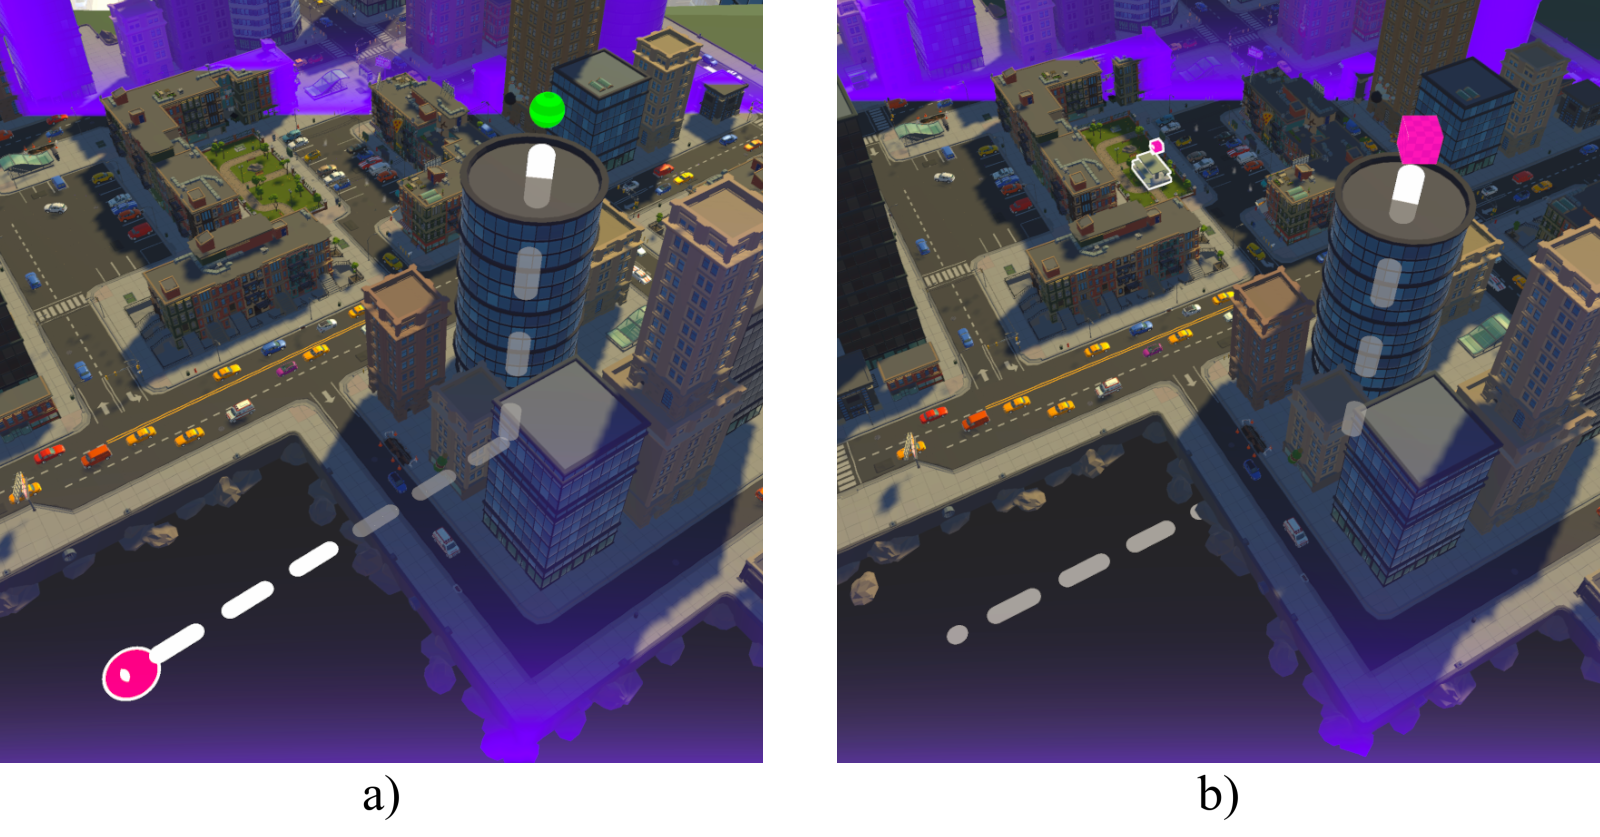
\includegraphics[width=1\textwidth]{figures/balloon_poi.png}
            \captionof{figure}{Balloon selection helper lines. Image (a) shows the balloon for the first user, and image (b) shows the balloon for the second user with the secondary hand removed.}
            \label{fig:balloon_poi}
        \end{figure}

        The balloon and the vertical helper line are also visible in the 3D model, as shown in Figure \ref{fig:balloon_world}, helping users understand the balloon's position in the real world. Both are not visible behind objects in the 3D model. The balloon scales with distance so users can see it from afar.

       \begin{figure}[h!]
            \centering
            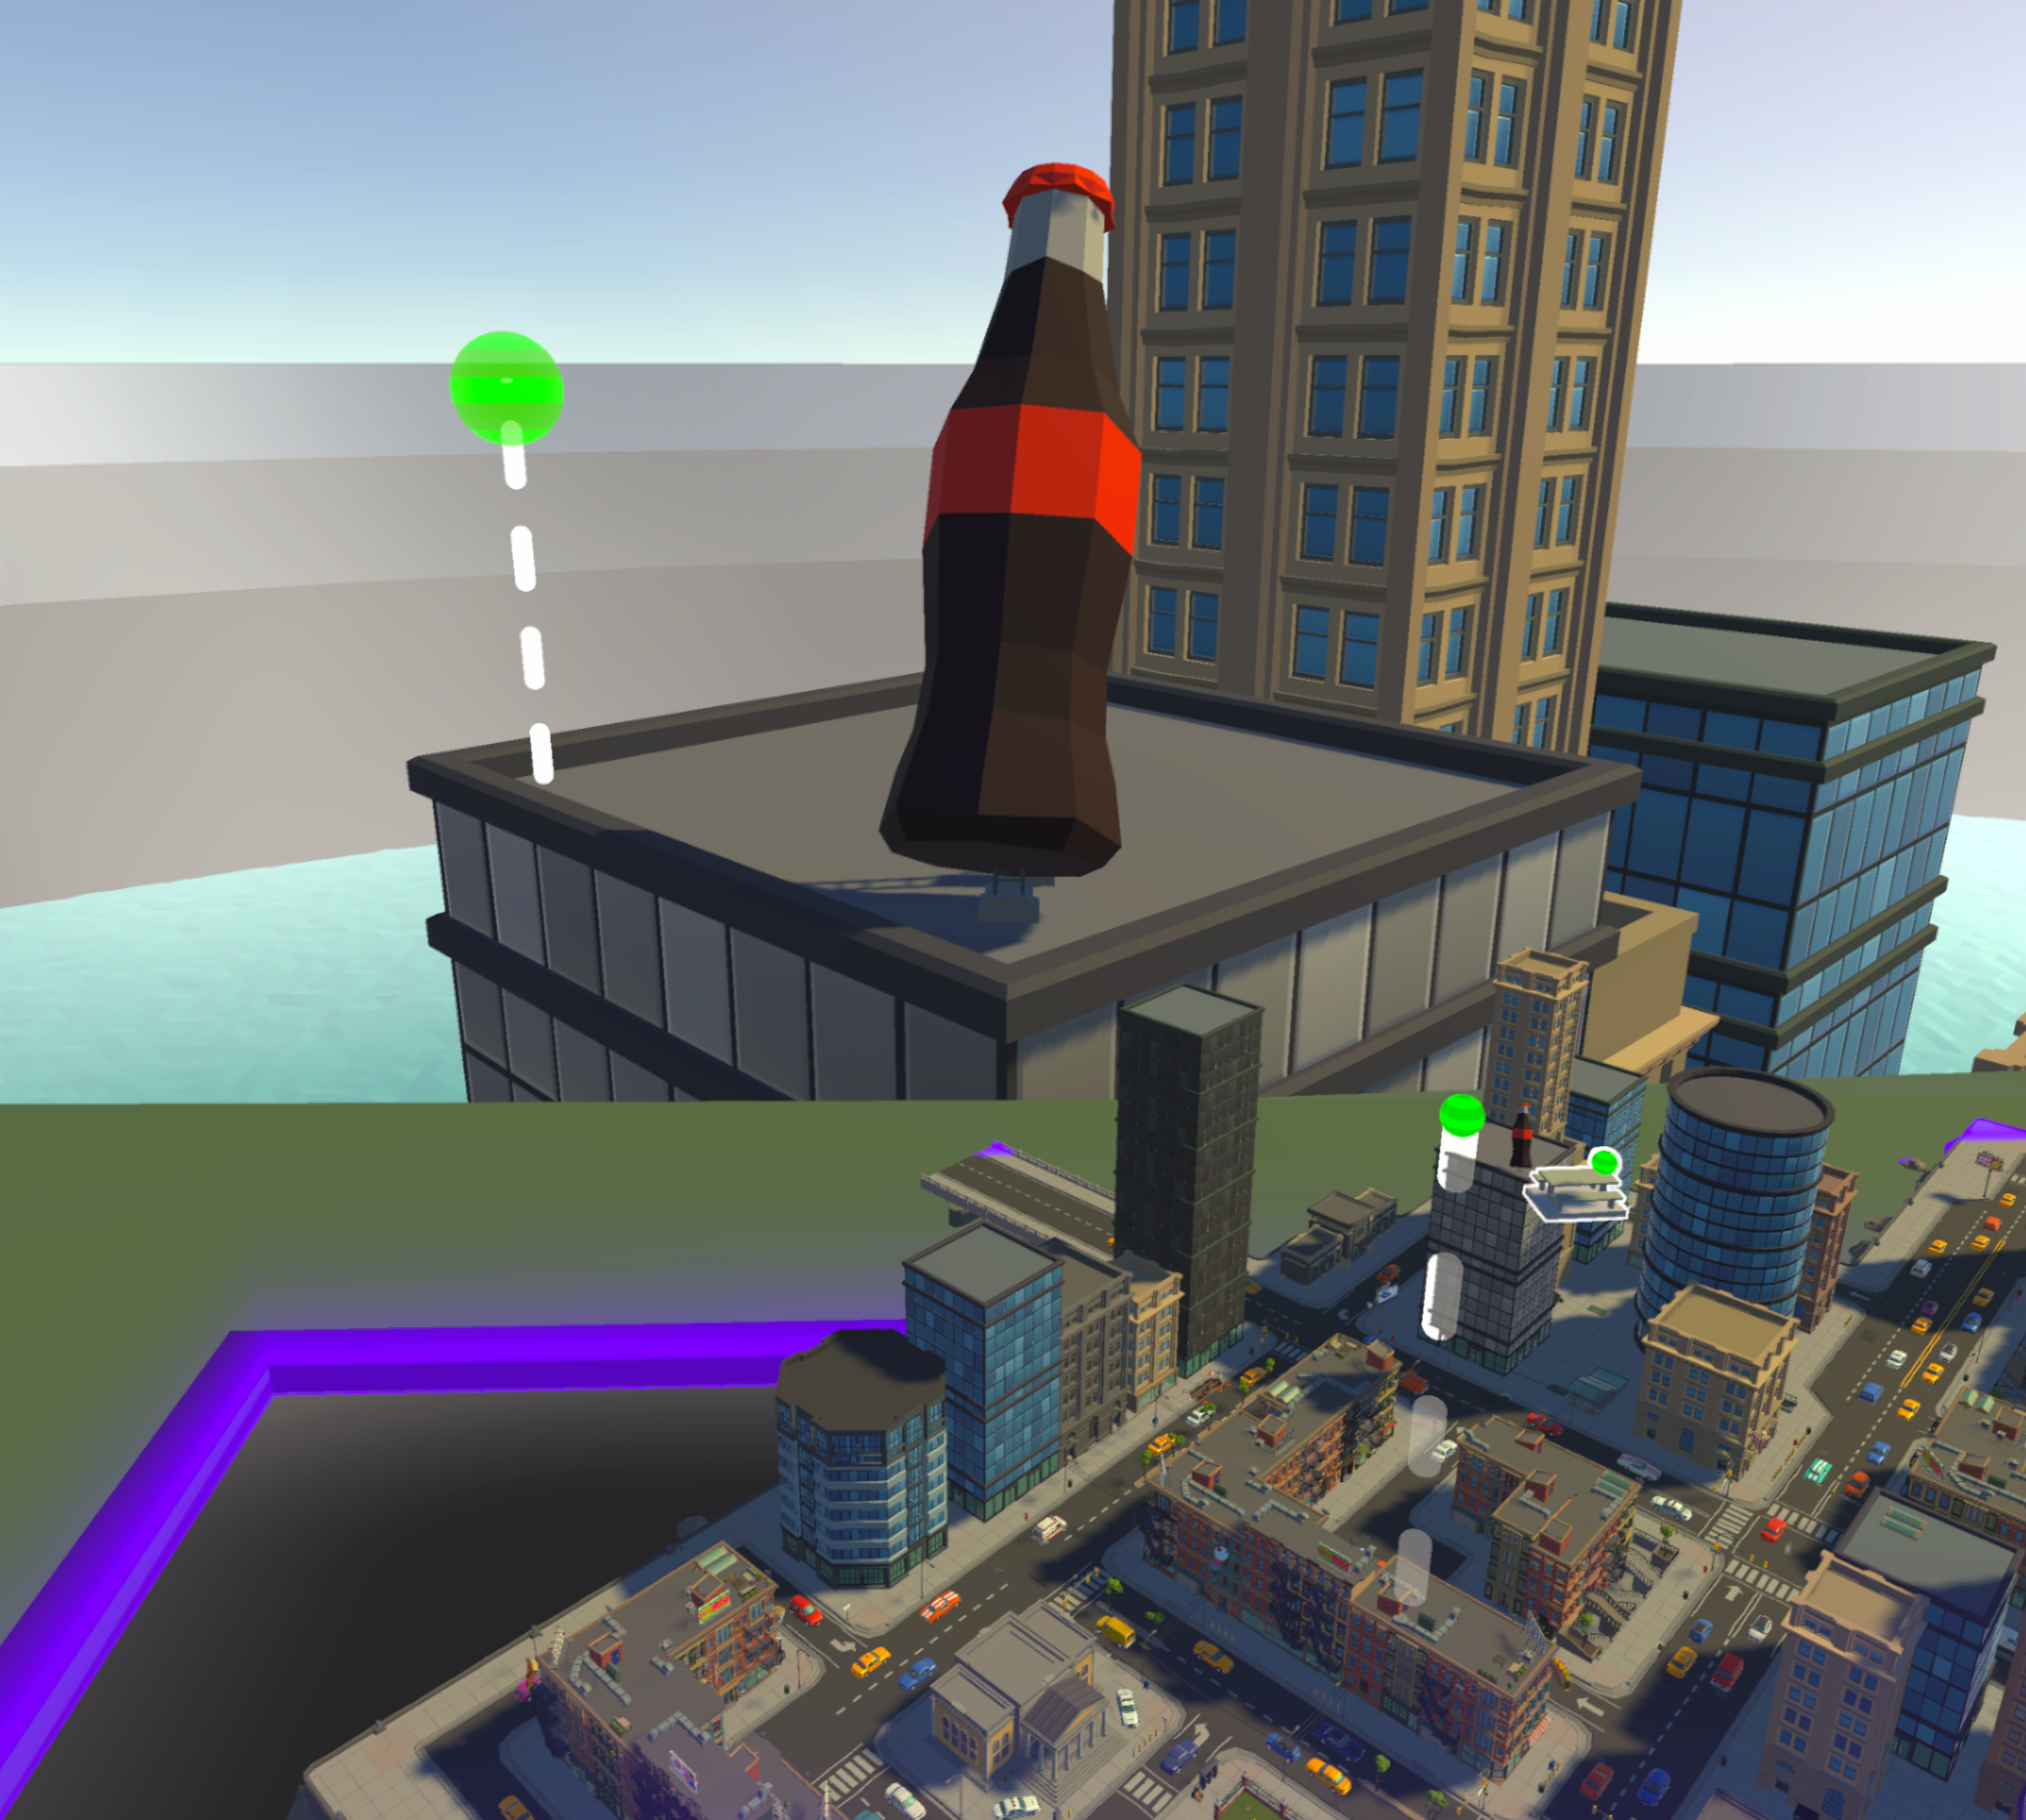
\includegraphics[width=1\textwidth]{figures/balloon_world.png}
            \captionof{figure}{Balloon selection visible both in the replica and in the 3D model.}
            \label{fig:balloon_world}
        \end{figure}
        
        When the balloon intersects a point of interest, the point of interest becomes outlined, indicating it is selected, as shown in image (a) of Figure \ref{fig:balloon_selection_intersection}. When the balloon intersects a table, the table grows in size, as shown in image (b) of Figure \ref{fig:balloon_selection_intersection}.

       \begin{figure}[h!]
            \centering
            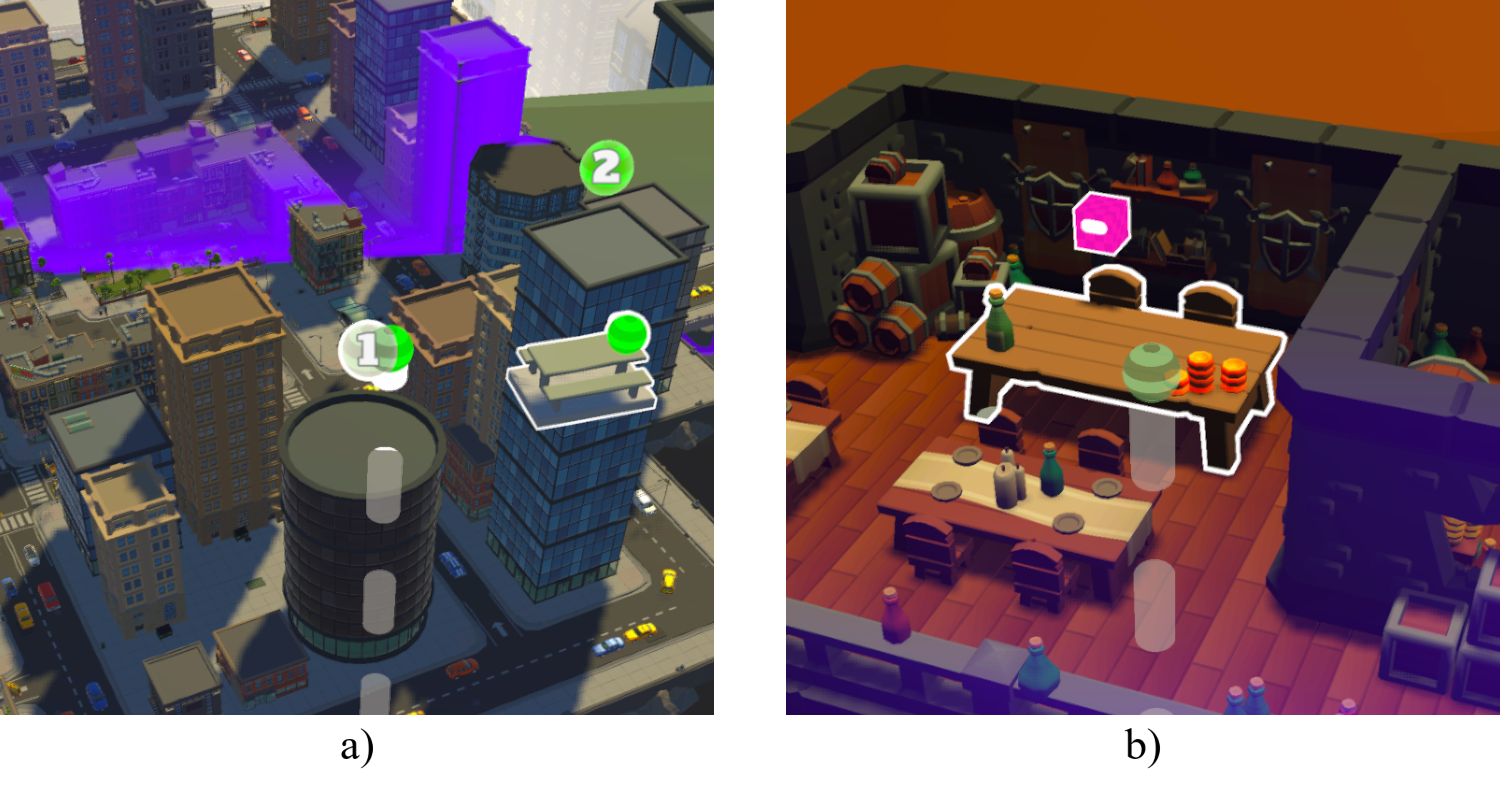
\includegraphics[width=1\textwidth]{figures/balloon_selection_intersection.png}
            \captionof{figure}{Balloon selection intersection with a point of interest in image a) and a table in image b).}
            \label{fig:balloon_selection_intersection}
        \end{figure}
    
\section{Networking}

    The prototype utilizes Unity's Netcode for GameObjects library to handle networking, enabling synchronization of GameObjects and Scenes across clients. This simplifies the management of the prototype's networking components. The networking architecture follows a client-server topology, illustrated in Figure \ref{fig:topology}. Specifically, it uses a client-hosted server named a host, where one client is also the server. This architecture was chosen for its simplicity in setup and management, and because it meets the prototype's requirements.

    \begin{figure}[h]
        \centering
        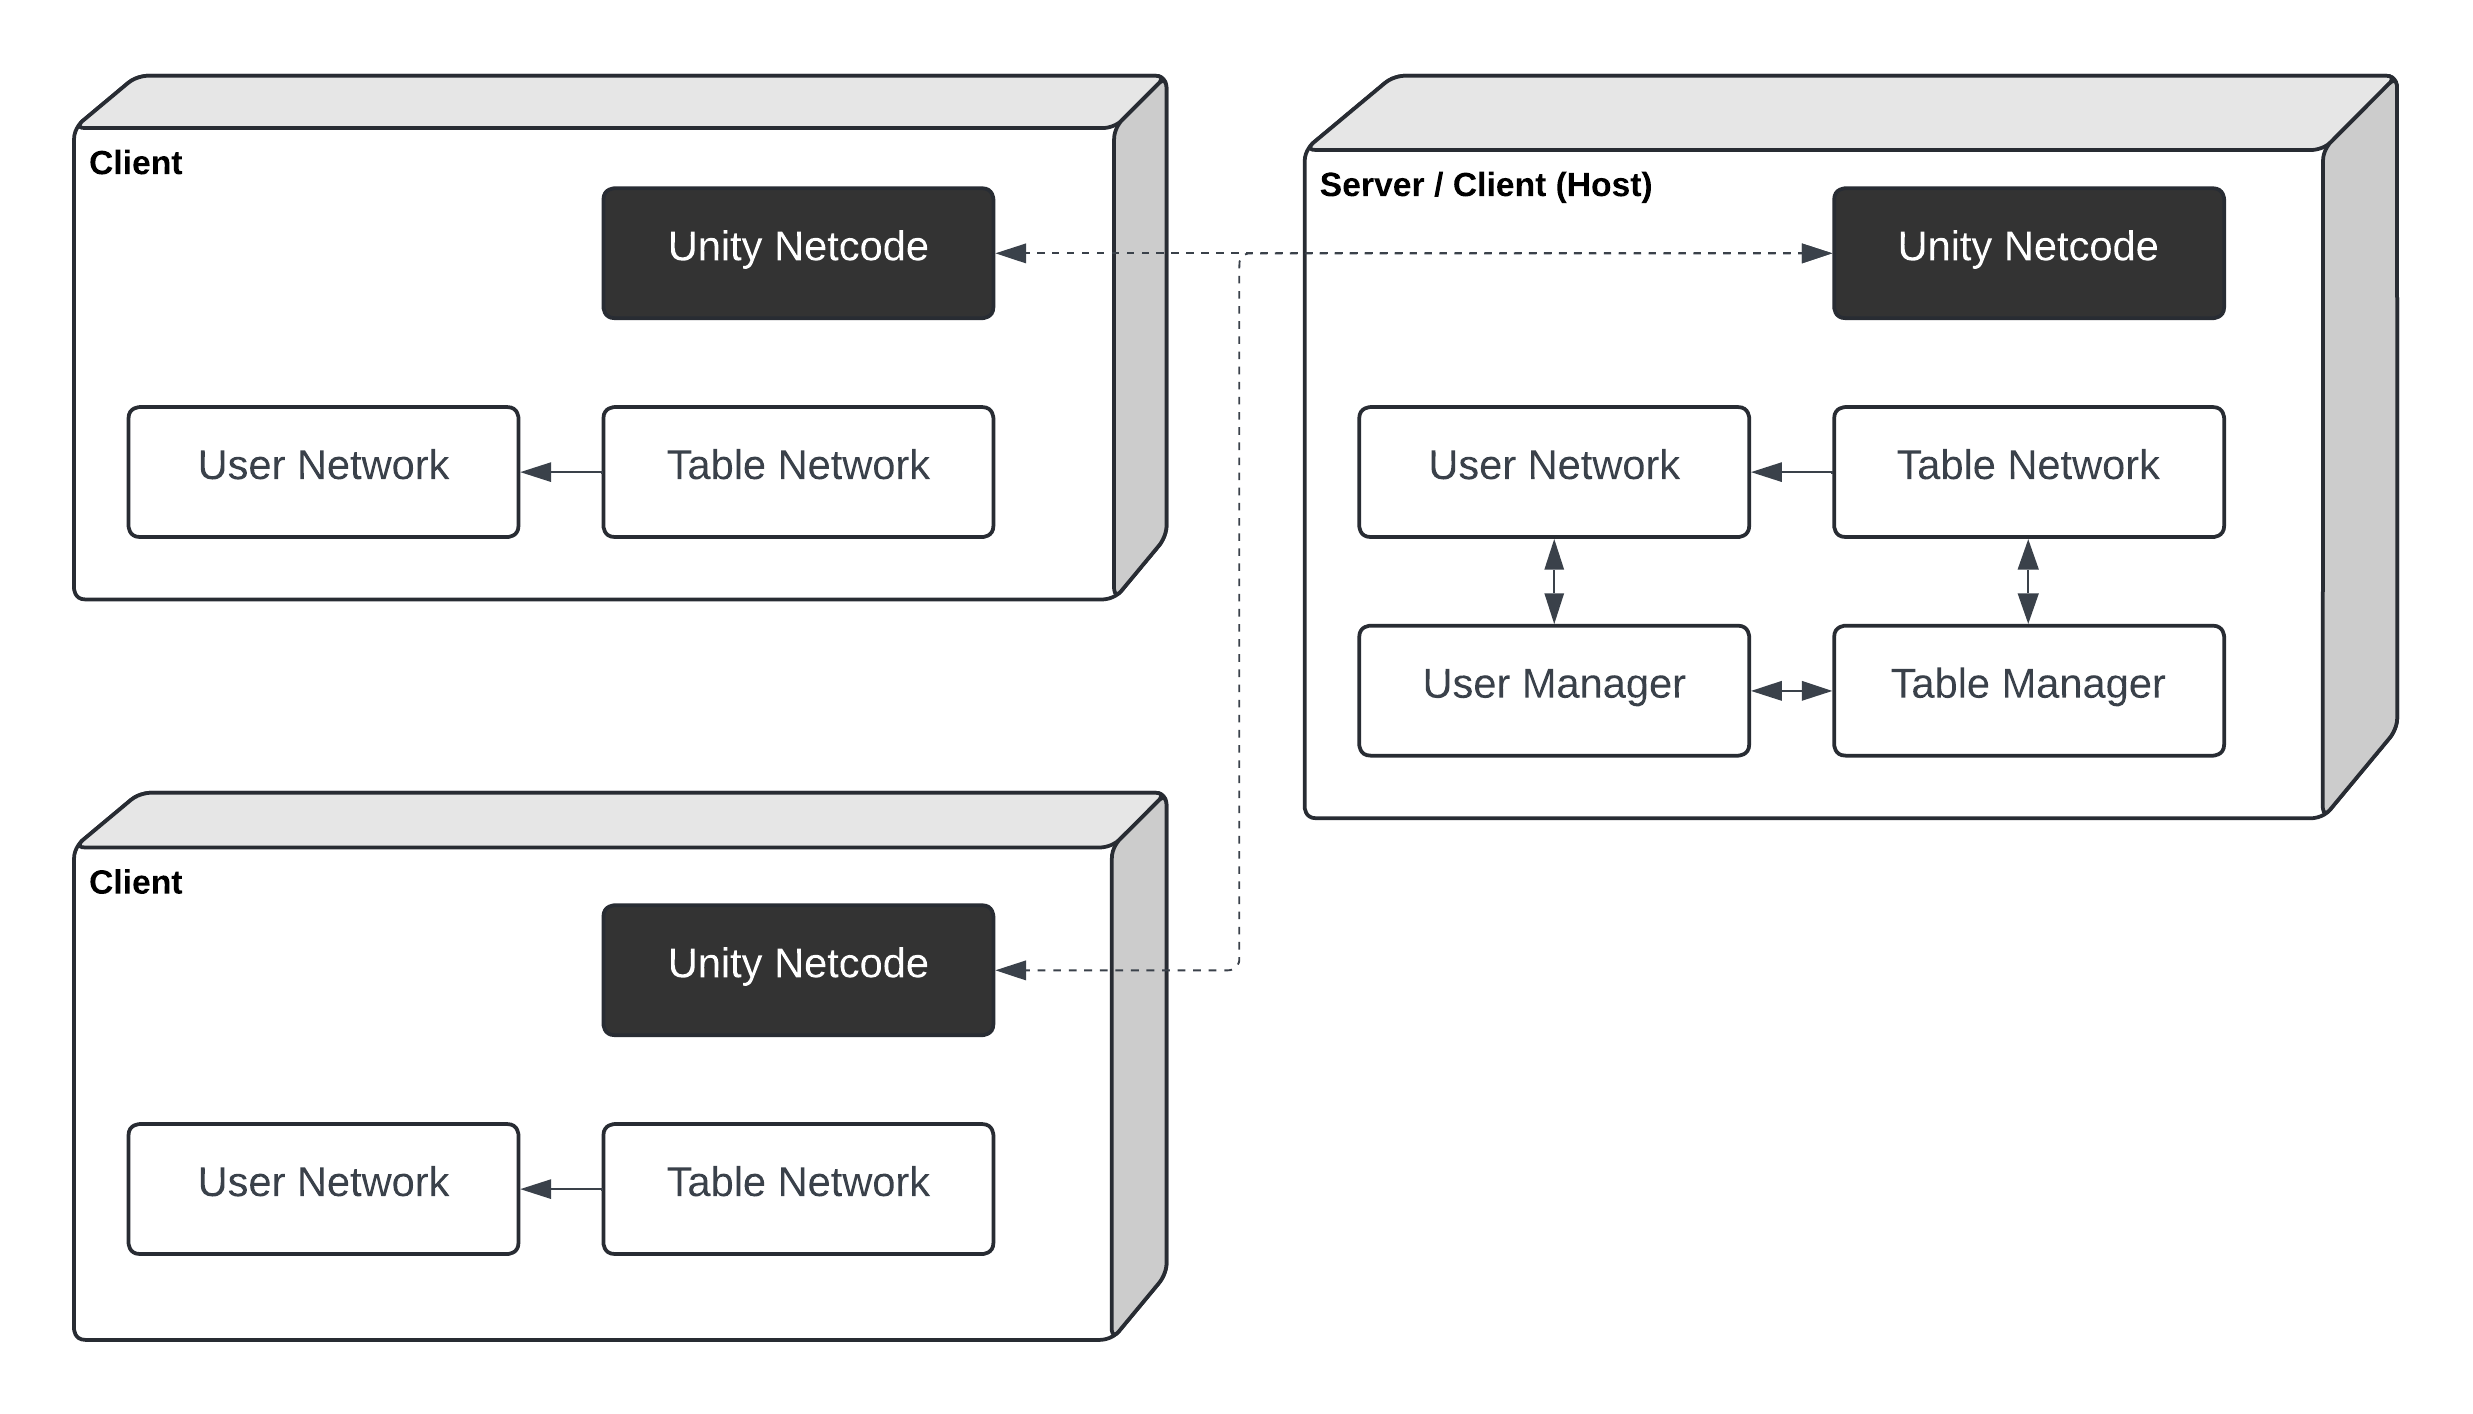
\includegraphics[width=.9\linewidth]{figures/topology.png}
        \caption{Networking architecture, using a client-server topology.}
        \label{fig:topology}
    \end{figure}

    Each client has a user network object for each connected user and a table network object for each table in the scene. A NetworkObject is a GameObject that interacts with Netcode. Before an instantiated NetworkObject is synchronized across clients, it must be spawned. In the client-server architecture, only the server has the authority to spawn and despawn NetworkObjects. By default, NetworkObjects are owned by the server and tied to its lifecycle. However, the user network objects are an exception. These are player NetworkObjects, that are automatically spawned by the server whenever a client connects, assigned to the client with ownership, and despawned when the client disconnects.\footnote{\url{https://docs-multiplayer.unity3d.com/netcode/current/basics/networkobject/}}


    NetworkObjects share data through network variables, synchronized with new clients when they join the server and with existing clients when the data changes. Network variables can have different permissions for reading and writing data. In a client-server architecture, the default setting is that the server has read-write permissions, while clients have read-only permissions.\footnote{\url{https://docs-multiplayer.unity3d.com/netcode/current/basics/networkvariable/}} Sections \ref{sec:user_network} and \ref{sec:table_network} describe the user and table network objects in detail. 

    The server manages the user and table network objects through the User Manager and Table Manager, respectively. These managers store data about connected users and tables, such as the association of user IDs to Netcode client IDs, the current point of interest ID, and the connected user IDs. They also handle the creation and destruction of network objects. Detailed functions of these managers are described in Sections \ref{sec:user_manager} and \ref{sec:table_manager}.

    The managers communicate with network objects through updates on network variables and remote procedure calls (RPCs). An RPC allows methods to be called on objects in another executable. In Netcode, RPCs execute methods on NetworkObjects across clients. A client can call an RPC on the server, and the server can call an RPC on a client. Clients can also call RPCs on other clients, though this passes through the server as a proxy.\footnote{\url{https://docs-multiplayer.unity3d.com/netcode/current/advanced-topics/message-system/rpc/}} Section \ref{sec:sequence_events} describes the sequence of events during the prototype's execution, including the RPCs used and other network-related events.

    \subsection{User Network Object} \label{sec:user_network}

        User network objects use network variables to store and synchronize data about the users. They have three network variables: user ID, a list of points of interest, and user transform data. The user ID identifies the user and determines their appearance. The list of points of interest contains the ID, position, and user ID of each point created by the user. The user transform data includes the user's position and rotation.

        The user ID and points of interest can only be modified by the server, while the user transform data is updated by the client. This design choice simplifies the synchronization of the table tracking algorithm described in Section \ref{sec:table_tracking}. The server assigns the user ID when the user joins, and updates the points of interest list as the user creates or removes points. The client updates the user transform data whenever the user moves.
        
        When a user network object receives an update to the user ID it updates the user's appearance. If the client owns the user network object, it also updates the balloon's appearance of the balloon selection.

        When a user creates a point of interest, a temporary point of interest is first created on the client, without an identification number, in both the replica and the 3D model. The temporary point of interest's position and user ID are sent to the user manager through an RPC. The user manager assigns an identification number to the point of interest and updates the appropriate user network object's points of interest list. Whenever this list is updated, the user network objects determine the type of update. If the client is the owner of the user network object and a point has been added, the temporary point of interest is updated with the identification number. If the client is not the owner, the replica controller is updated with the new point of interest, and marks it as unacknowledged. If a point of interest is removed, the user network object removes the point of interest from the replica controller. Late-joining users acquire all the spawned user network objects and update the WIM with the points of interest. 

    \subsection{Table Network Object} \label{sec:table_network}

        Table network objects have three network variables: transform data, the user ID seated at the first seat, and the user ID seated at the second seat. The transform data includes the table's position and rotation. Only the server can modify these variables, managed by the table manager. When a table network object is spawned, clients create a table replica in the WIM with the defined transform and seat data. When the table is despawned, the table replica is destroyed. Late-joining users acquire all the spawned table network objects and create table replicas accordingly.

        When the server updates the table network object's transform data, clients update the local table instance and the table replica's transform data. If a client is seated at the table, the client moves to the new position using the tracking data, as described in Section \ref{sec:table_tracking}. When the server updates the table network object's seat data, clients update the table replica to reflect who is seated at each seat.

    \subsection{User Manager} \label{sec:user_manager}
    
        The user manager is responsible for tracking and communicating with connected users. It maintains the association of user IDs to Netcode client IDs, the current point of interest ID, and the list of connected user IDs. When a user connects, Netcode triggers the \lstinline{OnClientConnected} event on the user manager, which assigns a user ID and updates the list of connected user IDs. For this prototype, only two users can be connected, so the user manager has a list of available user IDs, 0 and 1, which it assigns to new users. After updating the user's ID network variable, the user manager requests the table manager to add the player to an available table, as described in Section \ref{sec:table_manager}. Once a table is assigned, the user manager sends an RPC \lstinline{MoveUserToTableClientRpc} to the user network object to move the user to the table, as shown in Figures \ref{fig:connect_and_create} and \ref{fig:connect_and_join}. When a user disconnects, the user manager removes the user ID from the list of connected user IDs and adds it back to the list of available user IDs. It then requests the table manager to remove the player from their table, as depicted in Figure \ref{fig:disconnect}. The spawning and despawning of user network objects are handled automatically by Netcode.

        When a user creates a point of interest, the user's network object sends an \lstinline{CreatePointOf}\lstinline{InterestRpc} to the user manager. The user manager increments the current point of interest ID and updates the user network object's points of interest list. Because this list is a network variable, it is synchronized across all clients, and the user network object handles the update accordingly, as described in Section \ref{sec:user_network}. When a user removes a point of interest, the user network object sends an RPC \lstinline{RemovePointOfInterestRpc} to the user manager. The user manager then removes the point of interest from the network object's list.
        
        When a user teleports or joins a table, the user network object sends an \lstinline{MoveUserTo}\lstinline{PositionRpc} or \lstinline{MoveUserToTableRpc} to the user manager. The user manager then instructs the table manager to move the user to the new position or table, as outlined in Section \ref{sec:table_manager}. Afterward, the user manager sends an RPC \lstinline{MoveUserToTableClientRpc} to update the user network object's position, as illustrated in Figures \ref{fig:teleport} and \ref{fig:table_join}.

    \subsection{Table Manager} \label{sec:table_manager}

        The table manager oversees the table network objects and assigns users to tables. Its primary functions include assigning newly connected users to available tables, managing user teleportation, handling users joining tables, and removing users from tables upon disconnection.

        When assigning a user to a table, the table manager first checks for available seats at existing tables. If a seat is available, the user is assigned to it. If no seats are available, the table manager creates a new table and assigns the user to the first seat. These scenarios are depicted in Figures \ref{fig:connect_and_create} and \ref{fig:connect_and_join}. When a user disconnects, the table manager removes them from their table. If the table becomes empty, it is despawned. This process is illustrated in Figure \ref{fig:disconnect}.

        When handling user teleportation, the table manager first checks if the user is alone at their current table. If they are, it moves the table to the new position. If the user is not alone, a new table is created at the new position, and the user is assigned to the first seat. These scenarios are depicted in Figure \ref{fig:teleport}.

        When a user joins a table, the table manager removes them from their original table. If the original table becomes empty, it is despawned. The user is then assigned to the first available seat on the new table. This process is shown in Figure \ref{fig:table_join}.


    \subsection{Sequence of Events} \label{sec:sequence_events}

        This section outlines a typical scenario that demonstrates the key interactions between users, tables, and the network. The diagrams illustrated only show the interaction between one client and the server at a time, from the perspective of the owner of the depicted user network object. Whenever a network variable is updated, the change is synchronized across all clients.

        The scenario begins with a user creating a server, thereby becoming its host. In this case, RPCs are local and executed instantly since the server also functions as a client. The client then connects to the server, as shown in Figure \ref{fig:connect_and_create}. The user manager assigns the user the ID 0 by updating the user's network variable and the list of connected user IDs. Upon updating this ID, the user's model is updated to the correct appearance. The user manager then requests the table manager to assign the user to an available table. Since no other users are connected, the table manager creates a new table, Table Network 1, and assigns the user to the first seat. When the table is spawned, it requests the local client to create the table replica on the WIM. The user manager then sends an RPC to the user network object, moving the user to the table.

        \begin{figure}[h]
            \centering
            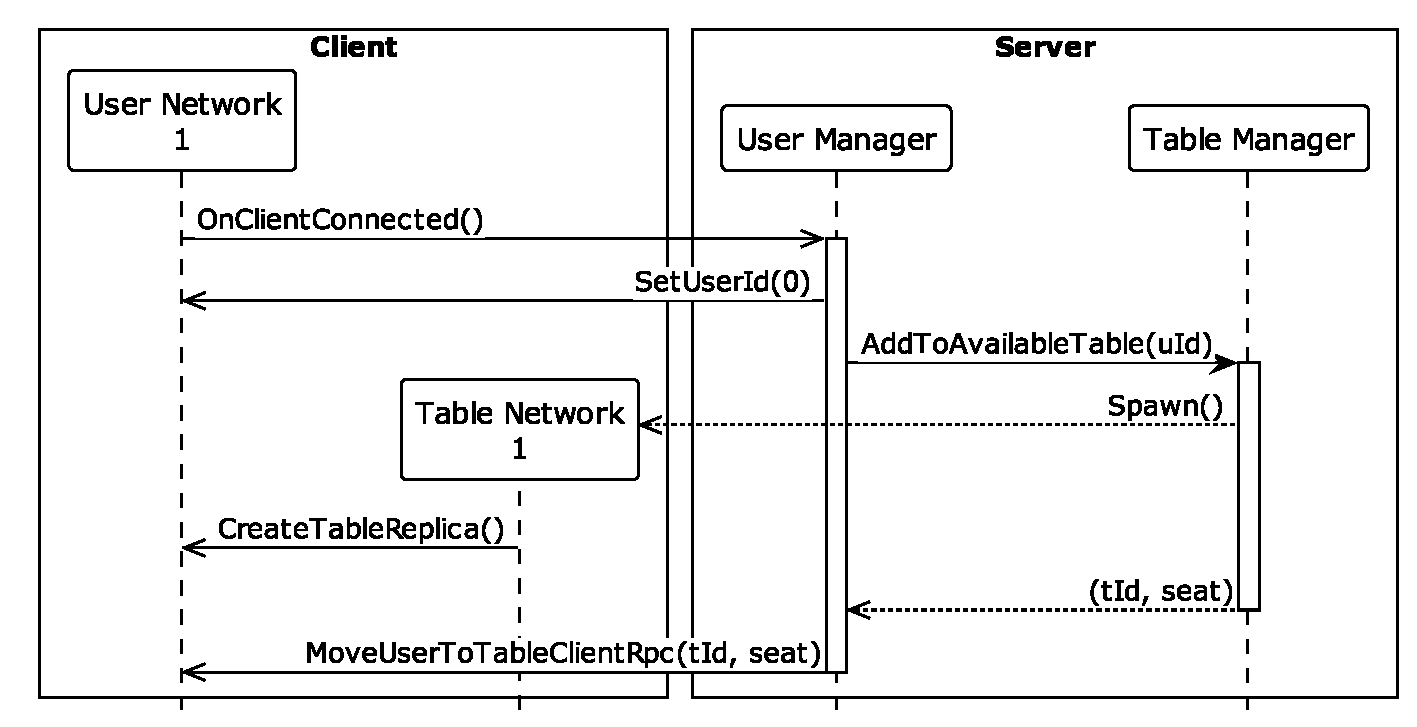
\includegraphics[width=.85\linewidth]{diagrams/out/connect_and_create_table.eps}
            \caption{Sequence diagram of a user connecting and creating a table.}
            \label{fig:connect_and_create}
        \end{figure}

        Next, the user creates a point of interest. Initially, a temporary point of interest is created on the client, followed by sending a \lstinline{CreatePointOfInterestRpc} to the user manager. The user manager increments the current point of interest ID and updates the user network's points of interest list. When the user network object receives this update, it assigns the identification number to the temporary point of interest, as it is owned by the client.

        The user then teleports to a new position. The user network object sends a \lstinline{MoveUserTo}\lstinline{PositionRpc} to the user manager, which instructs the table manager to move the user to the new location. Since the user is alone at the table, the table is moved to the new position, updating its network variables accordingly. The table network object, upon receiving these updates, adjusts the table replica on the client, and moves the user to the new position.

        \begin{figure}[h]
            \centering
            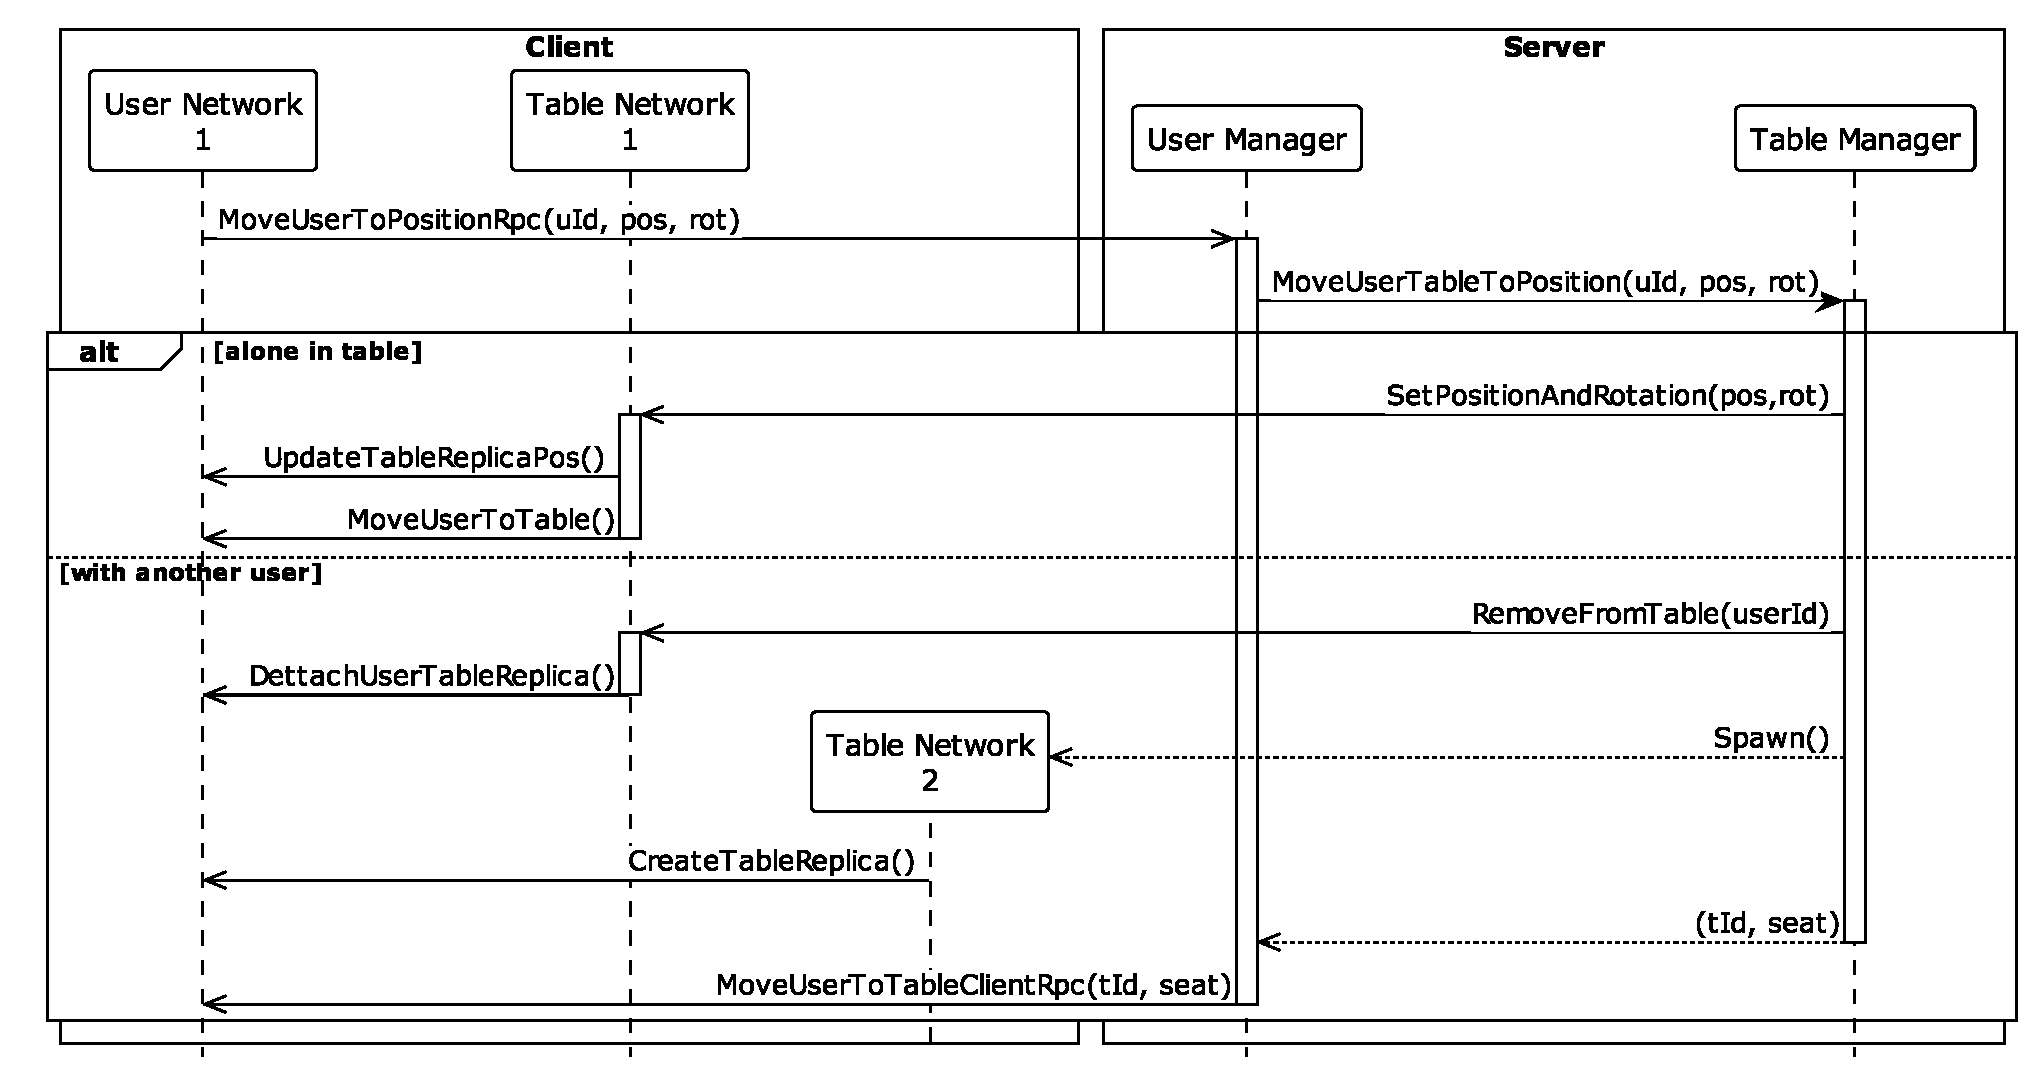
\includegraphics[width=.85\linewidth]{diagrams/out/teleport.eps}
            \caption{Sequence diagram of a user teleporting.}
            \label{fig:teleport}
        \end{figure}

        Later, another user connects to the server, as illustrated in Figure \ref{fig:connect_and_join}. The user manager assigns this user the ID 1 and updates the list of connected user IDs. Consequently, the user network object is updated with the new user ID and the corresponding appearance. The table manager assigns the new user to the second seat of Table Network 1, updating its seat network variables. The table network object then updates the table replica on each client, displaying the new user in the second seat. Following this, the user manager sends an RPC to the user network object to position the user at the table.

        \begin{figure}[ht!]
            \centering
            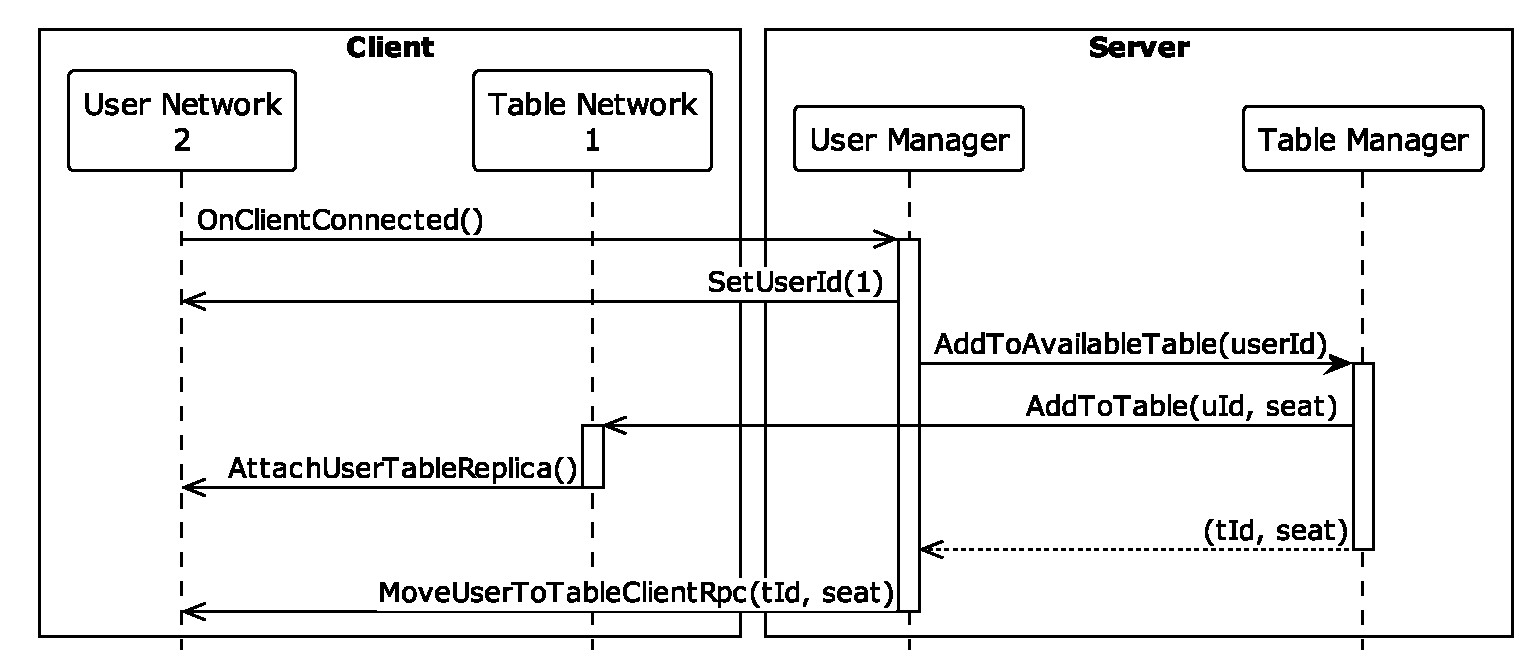
\includegraphics[width=.85\linewidth]{diagrams/out/connect_and_join_existing_table.eps}
            \caption{Sequence diagram of a user connecting and joining an existing table.}
            \label{fig:connect_and_join}
        \end{figure}

        Upon joining, the second user gathers information about the first user's points of interest by loading the point of interest data from the first user's network object, marking them as unacknowledged. Since acknowledgment data is local, no network communication is required. The second user would also load table data from other table network objects if any additional tables existed.

        Next, the first user moves to a new position, as depicted in Figure \ref{fig:teleport}. The user network object sends a \lstinline{MoveUserToPositionRpc} to the user manager, which instructs the table manager to relocate the user. Because the user is not alone at the table this time, the table manager removes the user from Table Network 1 and spawns a new table, Table Network 2, assigning the user to the first seat. The new table network object updates the table replica on each client to reflect the user's new position, while the old table network object removes the user from the replica. Finally, the user manager sends an RPC to the user network object, moving the user to the new table.

        Following this, the second user joins the second table, as shown in Figure \ref{fig:table_join}. Their network object sends a \lstinline{MoveUserToTableRpc} to the user manager, which instructs the table manager to move the user to the second table. The table manager removes the user from Table Network 1 and assigns them to the second seat of Table Network 2. Since Table Network 1 is now empty, it is despawned. The table network objects update the table replicas on each client accordingly. The user manager then sends an RPC to the user network object, positioning the user at the new table.
        
        \begin{figure}[h!]
            \centering
            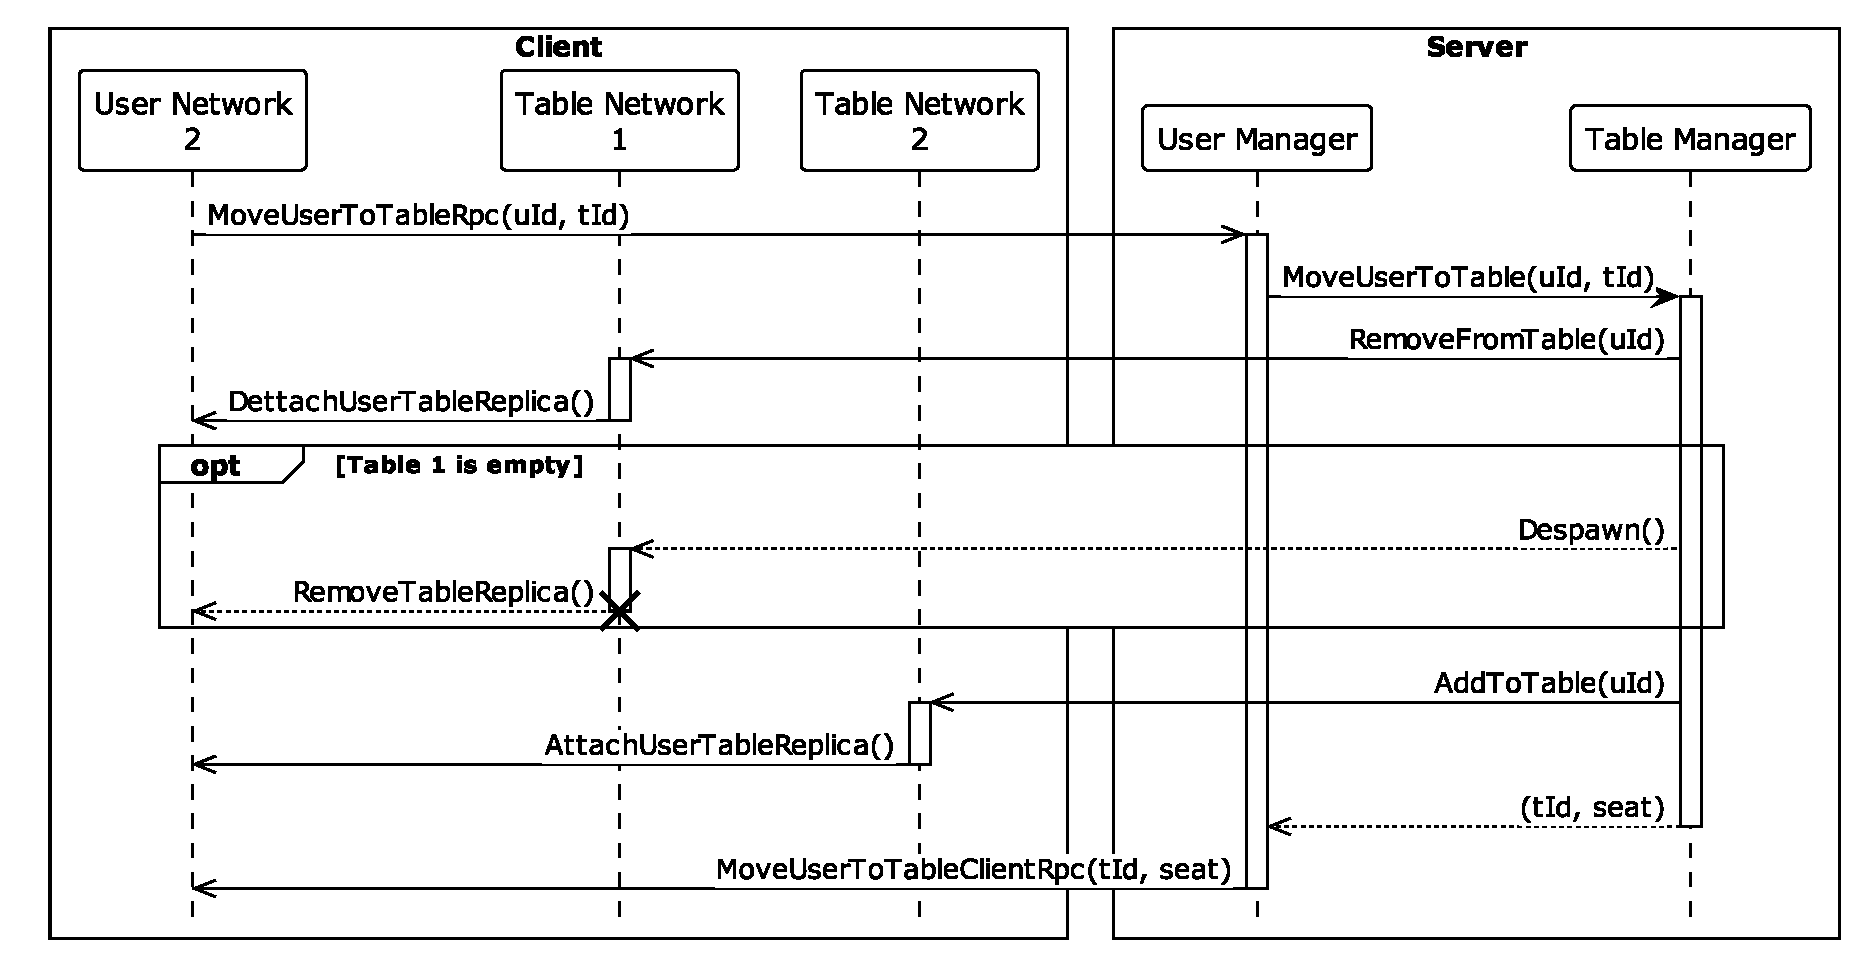
\includegraphics[width=.85\linewidth]{diagrams/out/table_join.eps}
            \caption{Sequence diagram of a user joining a table.}
            \label{fig:table_join}
        \end{figure}

        Finally, the first user disconnects, as depicted in Figure \ref{fig:disconnect}. The user manager removes the user ID from the list of connected user IDs and returns it to the list of available user IDs. It then instructs the table manager to remove the user from their table. The table network object updates the table replica on each client to reflect the user's removal. The user network object is automatically despawned by Netcode.

         \begin{figure}[h!]
            \centering
            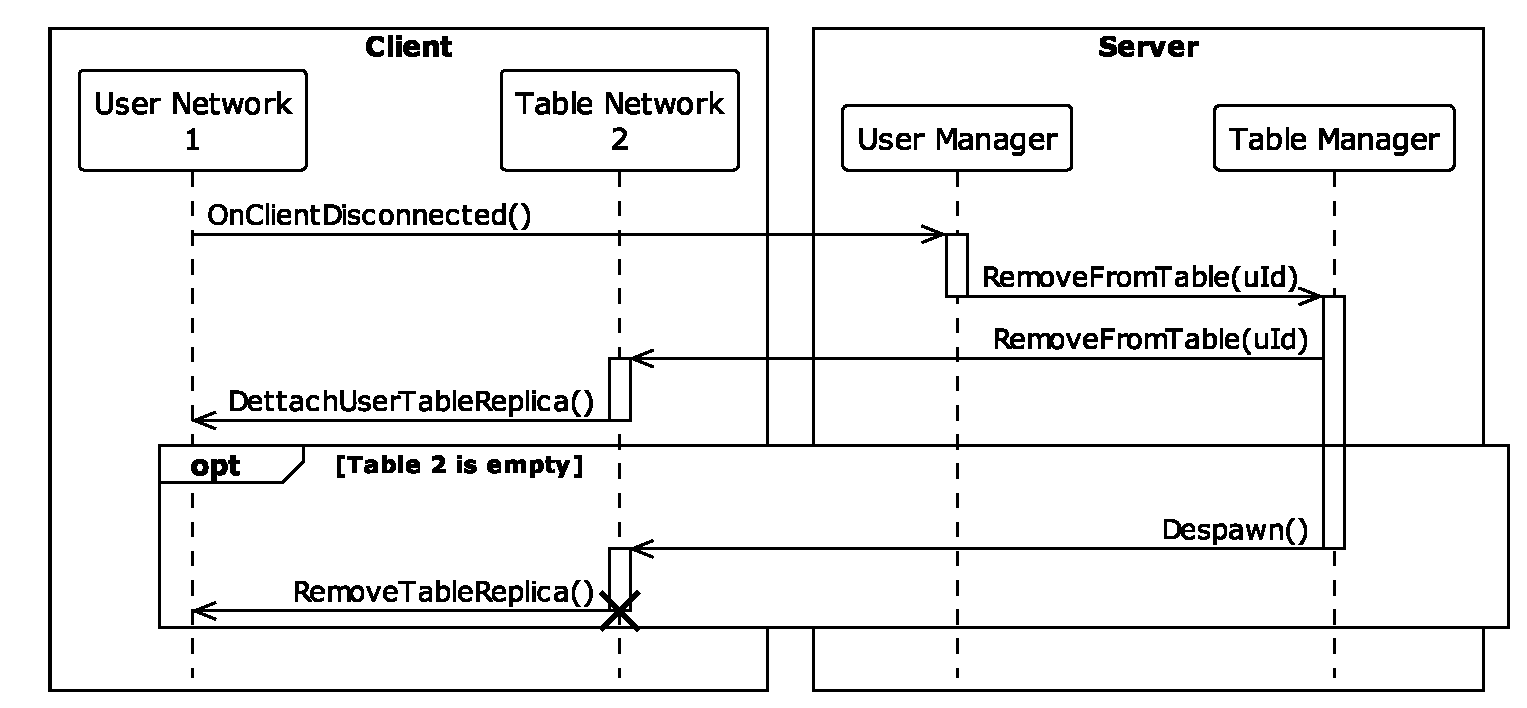
\includegraphics[width=.85\linewidth]{diagrams/out/disconnect.eps}
            \caption{Sequence diagram of a user disconnecting.}
            \label{fig:disconnect}
        \end{figure}

\section{Summary}
    This chapter details the implementation of a prototype for Replico. It starts with an overview of the system architecture and the hardware and software environment utilized, including Unity, Netcode for GameObjects, OpenXR, two HTC Vive Pro 2 headsets, and two multi-touch surfaces.

    The chapter continues by describing the state machine used to manage the prototype's states. These states range from the initial state, to \lstinline{TransformReplicaState} where users can manipulate the replica, and \lstinline{BalloonSelectionInitialState} where users can create, delete, and acknowledge points of interest, teleport, and join tables.

    Furthermore, the chapter details the calculations required to use the multi-touch input to transform the replica. Then, it details the gesture detection mechanisms used, including the utilization of the K-means clustering algorithm implemented via the ML.NET library for hand detection. Additionally, it outlines the use of VR controllers to track the user's interactions with virtual tables.

    The chapter describes the visual indicators implemented in the prototype. These include visual cues such as finger trails on the virtual touch frame, glow effects signaling gesture detection, illumination effects marking the touch frame's boundaries on the replica, and the visual representation of tables, table replicas, points of interest, and their corresponding visual appearances.

    The networking implementation is explained, describing the architecture, user and table network objects, user and table managers, network variables, and Remote Procedure Calls (RPCs). The section ends with an outline of a typical sequence of events that unfold during the prototype's operation.

\chapter{Evaluation}\label{chap:eval}

\section{Research Questions}

\section{Setup}

\section{Methodology}

    \subsection{Test Scenarios}

    \subsection{Tasks}

    \subsection{Data Logging}

        \subsubsection{Objective Data}

        \subsubsection{Subjective Data}

% do speak about how the frame being too sensitive to resting arms impacted the results
\chapter{Conclusions} \label{chap:concl}

This preparatory report for the dissertation explains the significance of fostering collaboration within DeskVR environments. It examines the foundational concepts of collaboration, explores methods to enhance communication in the digital realm, assesses the efficacy of VR in facilitating collaboration, and discusses the advantages and limitations specific to DeskVR.

Through a literature review, three primary themes were encountered. The first revolves around computer-supported cooperative work, investigating how users collaborate using computers. Within this topic, the exploration covered social translucence, workspace awareness, and the spatial model of interactions. The second area focused on concurrency control, which involves techniques used to preserve consistency amidst concurrent updates to objects. Three main approaches for concurrency control were detailed: object ownership, attribute separation, and distributed averages. The third area explored DeskVR interaction techniques, uncovering various methods for interacting with DeskVR environments, such as travel and object manipulation. This exploration provided insights into how to leverage DeskVR's constraints effectively.

The review highlights the potential value of creating replicas to enhance communication and maintain consistency in object arrangements within shared virtual environments in DeskVR. Moving forward, the next steps involve continuous experimentation with technology to refine the proposal, providing a deeper understanding of its requirements. The anticipated challenges encompass designing effective environmental interactions, presenting social information in a comprehensible and unobtrusive manner, and addressing the networking components. These challenges will guide the subsequent phases of research and experimentation.

% audio feedback
% multiple point deletion
% raycast look to to-scale model -> would help with making the to-scale model more used
% way to know own color
% help menu gestures
% ways to make accidental touches less significant
% people liked to see each other in the virtual environment
% teleport long press was confusing
    % in general it was confusing with many steps
% better implementation of the touch frame limits, as some people found it hard to know when it was in the limits
    % fade in from either inside or outside, instead of from the camera's direction
    % much harder to implement
% something nice, the hands should be color coded in the virtual touch frame -> for example primary hand are red, secondary hand are blue. in retrospect this makes immense sense, dumb idiot 

%%----------------------------------------
%% Final materials
%%----------------------------------------



%% Bibliography
%% Comment the next command if BibTeX file not used
%% bibliography is in ``myrefs.bib''
\PrintBib{myrefs}

%% 2021-07-20: change
%% comment next 2 commands if numbered appendices are not used
%\appendix
%\chapter{Appendix 1} \label{ap1:Lorem}


%% Index
%% Uncomment next command if index is required
%% don't forget to run ``makeindex thesis'' command
%\PrintIndex

\end{document}
